% Generated 2018-11-27 20:06:15 -0800
\subsection{Components} \label{model:Components}

\begin{figure}[ht]
  \centering
    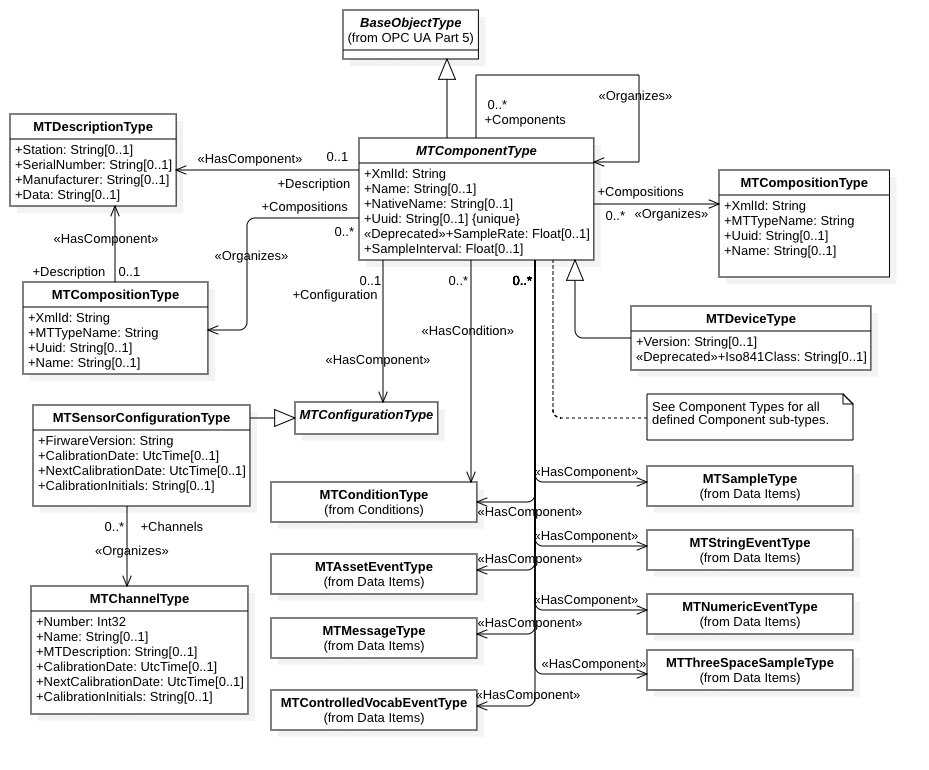
\includegraphics[width=1.0\textwidth]{./diagrams/types/Components.png}
  \caption{Components Diagram}
  \label{fig:Components}
\end{figure}

\FloatBarrier


The \glspl{MTComponent} documents the Component models and the owned objects.

\subsubsection{Defintion of \texttt{ MTChannelType}}
  \label{type:MTChannelType}

\FloatBarrier

A Channel of a sensor.

See ChannelType in type specifications.



\begin{table}[ht]
\centering 
  \caption{\texttt{MTChannelType} Definition}
  \label{table:MTChannelType}
\fontsize{9pt}{11pt}\selectfont
\tabulinesep=3pt
\begin{tabu} to 6in {|X[-1.35]|X[-0.7]|X[-1.75]|X[-1.5]|X[-1]|X[-0.7]|} \everyrow{\hline}
\hline
\rowfont\bfseries {Attribute} & \multicolumn{5}{|l|}{Value} \\
\tabucline[1.5pt]{}
BrowseName & \multicolumn{5}{|l|}{MTChannelType} \\
IsAbstract & \multicolumn{5}{|l|}{False} \\
\tabucline[1.5pt]{}
\rowfont \bfseries References & NodeClass & BrowseName & DataType & Type\-Definition & {Modeling\-Rule} \\
\multicolumn{6}{|l|}{Subtype of BaseObjectType (See \cite{UAPart5} Documentation)} \\
Has\-Property & Variable & Number & Int32 & Property\-Type & Mandatory \\
Has\-Property & Variable & Name & String & Property\-Type & Optional \\
Has\-Property & Variable & MT\-Description & String & Property\-Type & Optional \\
Has\-Property & Variable & Calibration\-Date & Utc\-Time & Property\-Type & Optional \\
Has\-Property & Variable & Next\-Calibration\-Date & Utc\-Time & Property\-Type & Optional \\
Has\-Property & Variable & Calibration\-Initials & String & Property\-Type & Optional \\
\end{tabu}
\end{table} 


\FloatBarrier
\subsubsection{Defintion of \texttt{ MTComponentType}}
  \label{type:MTComponentType}

\FloatBarrier

\begin{figure}[ht]
  \centering
    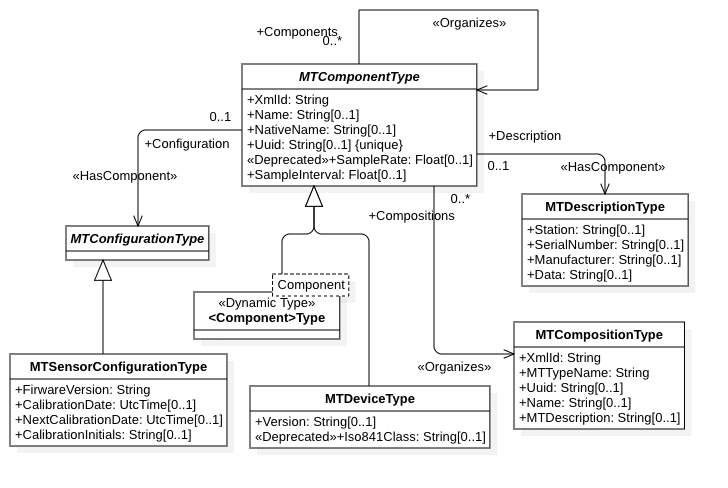
\includegraphics[width=1.0\textwidth]{./diagrams/types/MTComponentType.png}
  \caption{MTComponentType Diagram}
  \label{fig:MTComponentType}
\end{figure}

\FloatBarrier


The base \gls{MTComponent} Type from which all MTConnect Components are derived.
The component types will be created once for all \gls{MTComponent} \glspl{Object}
of that type based on the \gls{QName} of the MTConnect XML element. 

The Component Objects will be created and inserted into the \mtmodel{Components} 
folder with a \gls{BrowseName} of the Component \gls{QName} and the \mtmodel{name} element if specified surrounded 
by square brackets, \texttt{[]}. For example if the MTConnect Element is:

\xml{<Linear name='X'>...</...>}

The OPC UA Object with \gls{BrowseName} \xml{Linear[X]} will be created with the \uamodel{HasTypeDefinition}
referencing the \mtmodel{Linear} OPC UA \gls{Type}. 

The meta data for the component and its relationships are static. The dynamic data will be 
represented using the \cite{UAPart8}.



\begin{table}[ht]
\centering 
  \caption{\texttt{MTComponentType} Definition}
  \label{table:MTComponentType}
\fontsize{9pt}{11pt}\selectfont
\tabulinesep=3pt
\begin{tabu} to 6in {|X[-1.35]|X[-0.7]|X[-1.75]|X[-1.5]|X[-1]|X[-0.7]|} \everyrow{\hline}
\hline
\rowfont\bfseries {Attribute} & \multicolumn{5}{|l|}{Value} \\
\tabucline[1.5pt]{}
BrowseName & \multicolumn{5}{|l|}{MTComponentType} \\
IsAbstract & \multicolumn{5}{|l|}{True} \\
\tabucline[1.5pt]{}
\rowfont \bfseries References & NodeClass & BrowseName & DataType & Type\-Definition & {Modeling\-Rule} \\
\multicolumn{6}{|l|}{Subtype of BaseObjectType (See \cite{UAPart5} Documentation)} \\
HasSubtype & ObjectType & \multicolumn{2}{l}{MTDeviceType} & \multicolumn{2}{|l|}{See section \ref{type:MTDeviceType}} \\
HasSubtype & ObjectType & \multicolumn{2}{l}{<Component>Type} & \multicolumn{2}{|l|}{See section \ref{type:<Component>Type}} \\
Has\-Property & Variable & Xml\-Id & String & Property\-Type & Mandatory \\
Has\-Property & Variable & Name & String & Property\-Type & Optional \\
Has\-Property & Variable & Native\-Name & String & Property\-Type & Optional \\
Has\-Property & Variable & Uuid & String & Property\-Type & Optional \\
Has\-Property & Variable & Sample\-Rate & Float & Property\-Type & Optional \\
Has\-Property & Variable & Sample\-Interval & Float & Property\-Type & Optional \\
Has\-Component & Object & Description & \multicolumn{2}{l|}{MTDescriptionType} & Optional \\
Has\-Component & Object & Configuration & \multicolumn{2}{l|}{MTConfigurationType} & Optional \\
Has\-Component & Variable & <MT\-Controlled\-Vocab\-Event> & UInteger[] & MT\-Controlled\-Vocab\-Event\-Type & Optional \\
Has\-Component & Variable & <MT\-Numeric\-Event> & Number[] & MT\-Numeric\-Event\-Type & Optional \\
Has\-Component & Variable & <MT\-String\-Event> & String[] & MT\-String\-Event\-Type & Optional \\
Has\-Component & Variable & <MT\-Sample> & Number[] & MT\-Sample\-Type & Optional \\
Has\-Component & Event & <MT\-Message> & \multicolumn{2}{l|}{MTMessageType[]} & Optional \\
Has\-Component & Variable & <MT\-Asset\-Event> & Asset\-Event\-Data\-Type[] & MT\-Asset\-Event\-Type & Optional \\
Has\-Component & Event & <MT\-Condition> & \multicolumn{2}{l|}{MTConditionType[]} & Optional \\
Has\-Condition & Event & <MT\-Condition> & \multicolumn{2}{l|}{MTConditionType[]} & Optional \\
Has\-Component & Variable & <MT\-Three\-Space\-Sample> & Three\-Space\-Position\-Data\-Type[] & MT\-Three\-Space\-Sample\-Type & Optional \\
Organizes & Object & Components & MT\-Component\-Type[] & Folder\-Type & Optional \\
Organizes & Object & Compositions & MT\-Composition\-Type[] & Folder\-Type & Optional \\
\end{tabu}
\end{table} 


\FloatBarrier
\subsubsection{Defintion of \texttt{ MTDeviceType}}
  \label{type:MTDeviceType}

\FloatBarrier

\input ./type-sections/MTDeviceType.tex

\begin{table}[ht]
\centering 
  \caption{\texttt{MTDeviceType} Definition}
  \label{table:MTDeviceType}
\fontsize{9pt}{11pt}\selectfont
\tabulinesep=3pt
\begin{tabu} to 6in {|X[-1.35]|X[-0.7]|X[-1.75]|X[-1.5]|X[-1]|X[-0.7]|} \everyrow{\hline}
\hline
\rowfont\bfseries {Attribute} & \multicolumn{5}{|l|}{Value} \\
\tabucline[1.5pt]{}
BrowseName & \multicolumn{5}{|l|}{MTDeviceType} \\
IsAbstract & \multicolumn{5}{|l|}{False} \\
\tabucline[1.5pt]{}
\rowfont \bfseries References & NodeClass & BrowseName & DataType & Type\-Definition & {Modeling\-Rule} \\
\multicolumn{6}{|l|}{Subtype of MTComponentType (See section \ref{type:MTComponentType})} \\
Has\-Property & Variable & Version & String & Property\-Type & Optional \\
Has\-Property & Variable & Iso841Class & String & Property\-Type & Optional \\
\end{tabu}
\end{table} 


\paragraph{Constraints}
\begin{itemize}
\item Constraint \texttt{uuid_not_empty}: 
   \indent \begin{lstlisting}
uuid->notEmpty()
\end{lstlisting}
Documentation: The  UUID SHALL be provided.

\end{itemize}
\begin{itemize}
\item Constraint \texttt{name_not_empty}: 
   \indent \begin{lstlisting}
name->notEmpty()
\end{lstlisting}
Documentation: The name of the Device SHALL be given.

\end{itemize}
\FloatBarrier
\subsubsection{Defintion of \texttt{<<Dynamic Type>> <Component>Type}}
  \label{type:<Component>Type}

\FloatBarrier

This is a dynamic type that will be created at the time the model is created.

The \gls{BrowseName} will be created using the \gls{QName} of the MTConnect \gls{MTComponent} element.
More information on the MTConnect \glspl{MTComponent} can be found in MTConnect Part 2 \cite{MTCPart2}.

\begin{table}[ht]
\centering 
  \caption{\texttt{<Component>Type} Definition}
  \label{table:<Component>Type}
\fontsize{9pt}{11pt}\selectfont
\tabulinesep=3pt
\begin{tabu} to 6in {|X[-1.35]|X[-0.7]|X[-1.75]|X[-1.5]|X[-1]|X[-0.7]|} \everyrow{\hline}
\hline
\rowfont\bfseries {Attribute} & \multicolumn{5}{|l|}{Value} \\
\tabucline[1.5pt]{}
BrowseName & \multicolumn{5}{|l|}{<Component>Type} \\
IsAbstract & \multicolumn{5}{|l|}{False} \\
\tabucline[1.5pt]{}
\rowfont \bfseries References & NodeClass & BrowseName & DataType & Type\-Definition & {Modeling\-Rule} \\
\multicolumn{6}{|l|}{Subtype of MTComponentType (See section \ref{type:MTComponentType})} \\
\end{tabu}
\end{table} 


\FloatBarrier
\subsubsection{Defintion of \texttt{ MTCompositionType}}
  \label{type:MTCompositionType}

\FloatBarrier

The \mtmodel{MTCompositionType} represents all composition entities. The specification of how
to form the \gls{BrowseName} is specified in Section~\ref{sec:browse-name-rules}.

The data items are added to the relationship where the \gls{MTDataItem} to \gls{Composition} 
relationship is represented by the \gls{BrowseName} Composition property of the data item.
The data items are added to the \gls{Composition} by their \glspl{BrowseName}.

\begin{table}[ht]
\centering 
  \caption{\texttt{MTCompositionType} Definition}
  \label{table:MTCompositionType}
\fontsize{9pt}{11pt}\selectfont
\tabulinesep=3pt
\begin{tabu} to 6in {|X[-1.35]|X[-0.7]|X[-1.75]|X[-1.5]|X[-1]|X[-0.7]|} \everyrow{\hline}
\hline
\rowfont\bfseries {Attribute} & \multicolumn{5}{|l|}{Value} \\
\tabucline[1.5pt]{}
BrowseName & \multicolumn{5}{|l|}{MTCompositionType} \\
IsAbstract & \multicolumn{5}{|l|}{False} \\
\tabucline[1.5pt]{}
\rowfont \bfseries References & NodeClass & BrowseName & DataType & Type\-Definition & {Modeling\-Rule} \\
\multicolumn{6}{|l|}{Subtype of BaseObjectType (See \cite{UAPart5} Documentation)} \\
Has\-Property & Variable & Xml\-Id & String & Property\-Type & Mandatory \\
Has\-Property & Variable & MT\-Type\-Name & String & Property\-Type & Mandatory \\
Has\-Property & Variable & Uuid & String & Property\-Type & Optional \\
Has\-Property & Variable & Name & String & Property\-Type & Optional \\
Has\-Property & Variable & MT\-Description & String & Property\-Type & Optional \\
\end{tabu}
\end{table} 


\FloatBarrier
\subsubsection{Defintion of \texttt{ MTConfigurationType}}
  \label{type:MTConfigurationType}

\FloatBarrier

The abstract \mtuatype{MTConfigurationType} currently has only one sub-type, \\
\mtuatype{MTSensorConfigurationType}. In the future, the configurations will also contain component 
and device configuration information as sub-types. 

\begin{table}[ht]
\centering 
  \caption{\texttt{MTConfigurationType} Definition}
  \label{table:MTConfigurationType}
\fontsize{9pt}{11pt}\selectfont
\tabulinesep=3pt
\begin{tabu} to 6in {|X[-1.35]|X[-0.7]|X[-1.75]|X[-1.5]|X[-1]|X[-0.7]|} \everyrow{\hline}
\hline
\rowfont\bfseries {Attribute} & \multicolumn{5}{|l|}{Value} \\
\tabucline[1.5pt]{}
BrowseName & \multicolumn{5}{|l|}{MTConfigurationType} \\
IsAbstract & \multicolumn{5}{|l|}{True} \\
\tabucline[1.5pt]{}
\rowfont \bfseries References & NodeClass & BrowseName & DataType & Type\-Definition & {Modeling\-Rule} \\
\multicolumn{6}{|l|}{Subtype of BaseObjectType (See \cite{UAPart5} Documentation)} \\
HasSubtype & ObjectType & \multicolumn{2}{l}{MTSensorConfigurationType} & \multicolumn{2}{|l|}{See section \ref{type:MTSensorConfigurationType}} \\
\end{tabu}
\end{table} 


\FloatBarrier
\subsubsection{Defintion of \texttt{ MTSensorConfigurationType}}
  \label{type:MTSensorConfigurationType}

\FloatBarrier

An MTConnect Sensor Configuration associated with the Component.

See SensorConfigurationType in type-specifications.

\begin{table}[ht]
\centering 
  \caption{\texttt{MTSensorConfigurationType} Definition}
  \label{table:MTSensorConfigurationType}
\fontsize{9pt}{11pt}\selectfont
\tabulinesep=3pt
\begin{tabu} to 6in {|X[-1.35]|X[-0.7]|X[-1.75]|X[-1.5]|X[-1]|X[-0.7]|} \everyrow{\hline}
\hline
\rowfont\bfseries {Attribute} & \multicolumn{5}{|l|}{Value} \\
\tabucline[1.5pt]{}
BrowseName & \multicolumn{5}{|l|}{MTSensorConfigurationType} \\
IsAbstract & \multicolumn{5}{|l|}{False} \\
\tabucline[1.5pt]{}
\rowfont \bfseries References & NodeClass & BrowseName & DataType & Type\-Definition & {Modeling\-Rule} \\
\multicolumn{6}{|l|}{Subtype of MTConfigurationType (See section \ref{type:MTConfigurationType})} \\
Has\-Property & Variable & Firware\-Version & String & Property\-Type & Mandatory \\
Has\-Property & Variable & Calibration\-Date & Utc\-Time & Property\-Type & Optional \\
Has\-Property & Variable & Next\-Calibration\-Date & Utc\-Time & Property\-Type & Optional \\
Has\-Property & Variable & Calibration\-Initials & String & Property\-Type & Optional \\
Organizes & Object & Channels & MT\-Channel\-Type[] & Folder\-Type & Optional \\
\end{tabu}
\end{table} 


\FloatBarrier
\subsubsection{Defintion of \texttt{ MTDescriptionType}}
  \label{type:MTDescriptionType}

\FloatBarrier

An MTConnect Component Description.

See the DescriptionType in the type-specifications.

\begin{table}[ht]
\centering 
  \caption{\texttt{MTDescriptionType} Definition}
  \label{table:MTDescriptionType}
\fontsize{9pt}{11pt}\selectfont
\tabulinesep=3pt
\begin{tabu} to 6in {|X[-1.35]|X[-0.7]|X[-1.75]|X[-1.5]|X[-1]|X[-0.7]|} \everyrow{\hline}
\hline
\rowfont\bfseries {Attribute} & \multicolumn{5}{|l|}{Value} \\
\tabucline[1.5pt]{}
BrowseName & \multicolumn{5}{|l|}{MTDescriptionType} \\
IsAbstract & \multicolumn{5}{|l|}{False} \\
\tabucline[1.5pt]{}
\rowfont \bfseries References & NodeClass & BrowseName & DataType & Type\-Definition & {Modeling\-Rule} \\
\multicolumn{6}{|l|}{Subtype of BaseObjectType (See \cite{UAPart5} Documentation)} \\
Has\-Property & Variable & Station & String & Property\-Type & Optional \\
Has\-Property & Variable & Serial\-Number & String & Property\-Type & Optional \\
Has\-Property & Variable & Manufacturer & String & Property\-Type & Optional \\
Has\-Property & Variable & Data & String & Property\-Type & Optional \\
\end{tabu}
\end{table} 


\FloatBarrier
\paragraph{Referenced Properties and Objects}

\begin{itemize}
\item \texttt{Data::String:} From the CDATA of the Description Element in MTConnect.

\end{itemize}
\FloatBarrier
\subsection{Data Items} \label{model:DataItems}

\begin{figure}[ht]
  \centering
    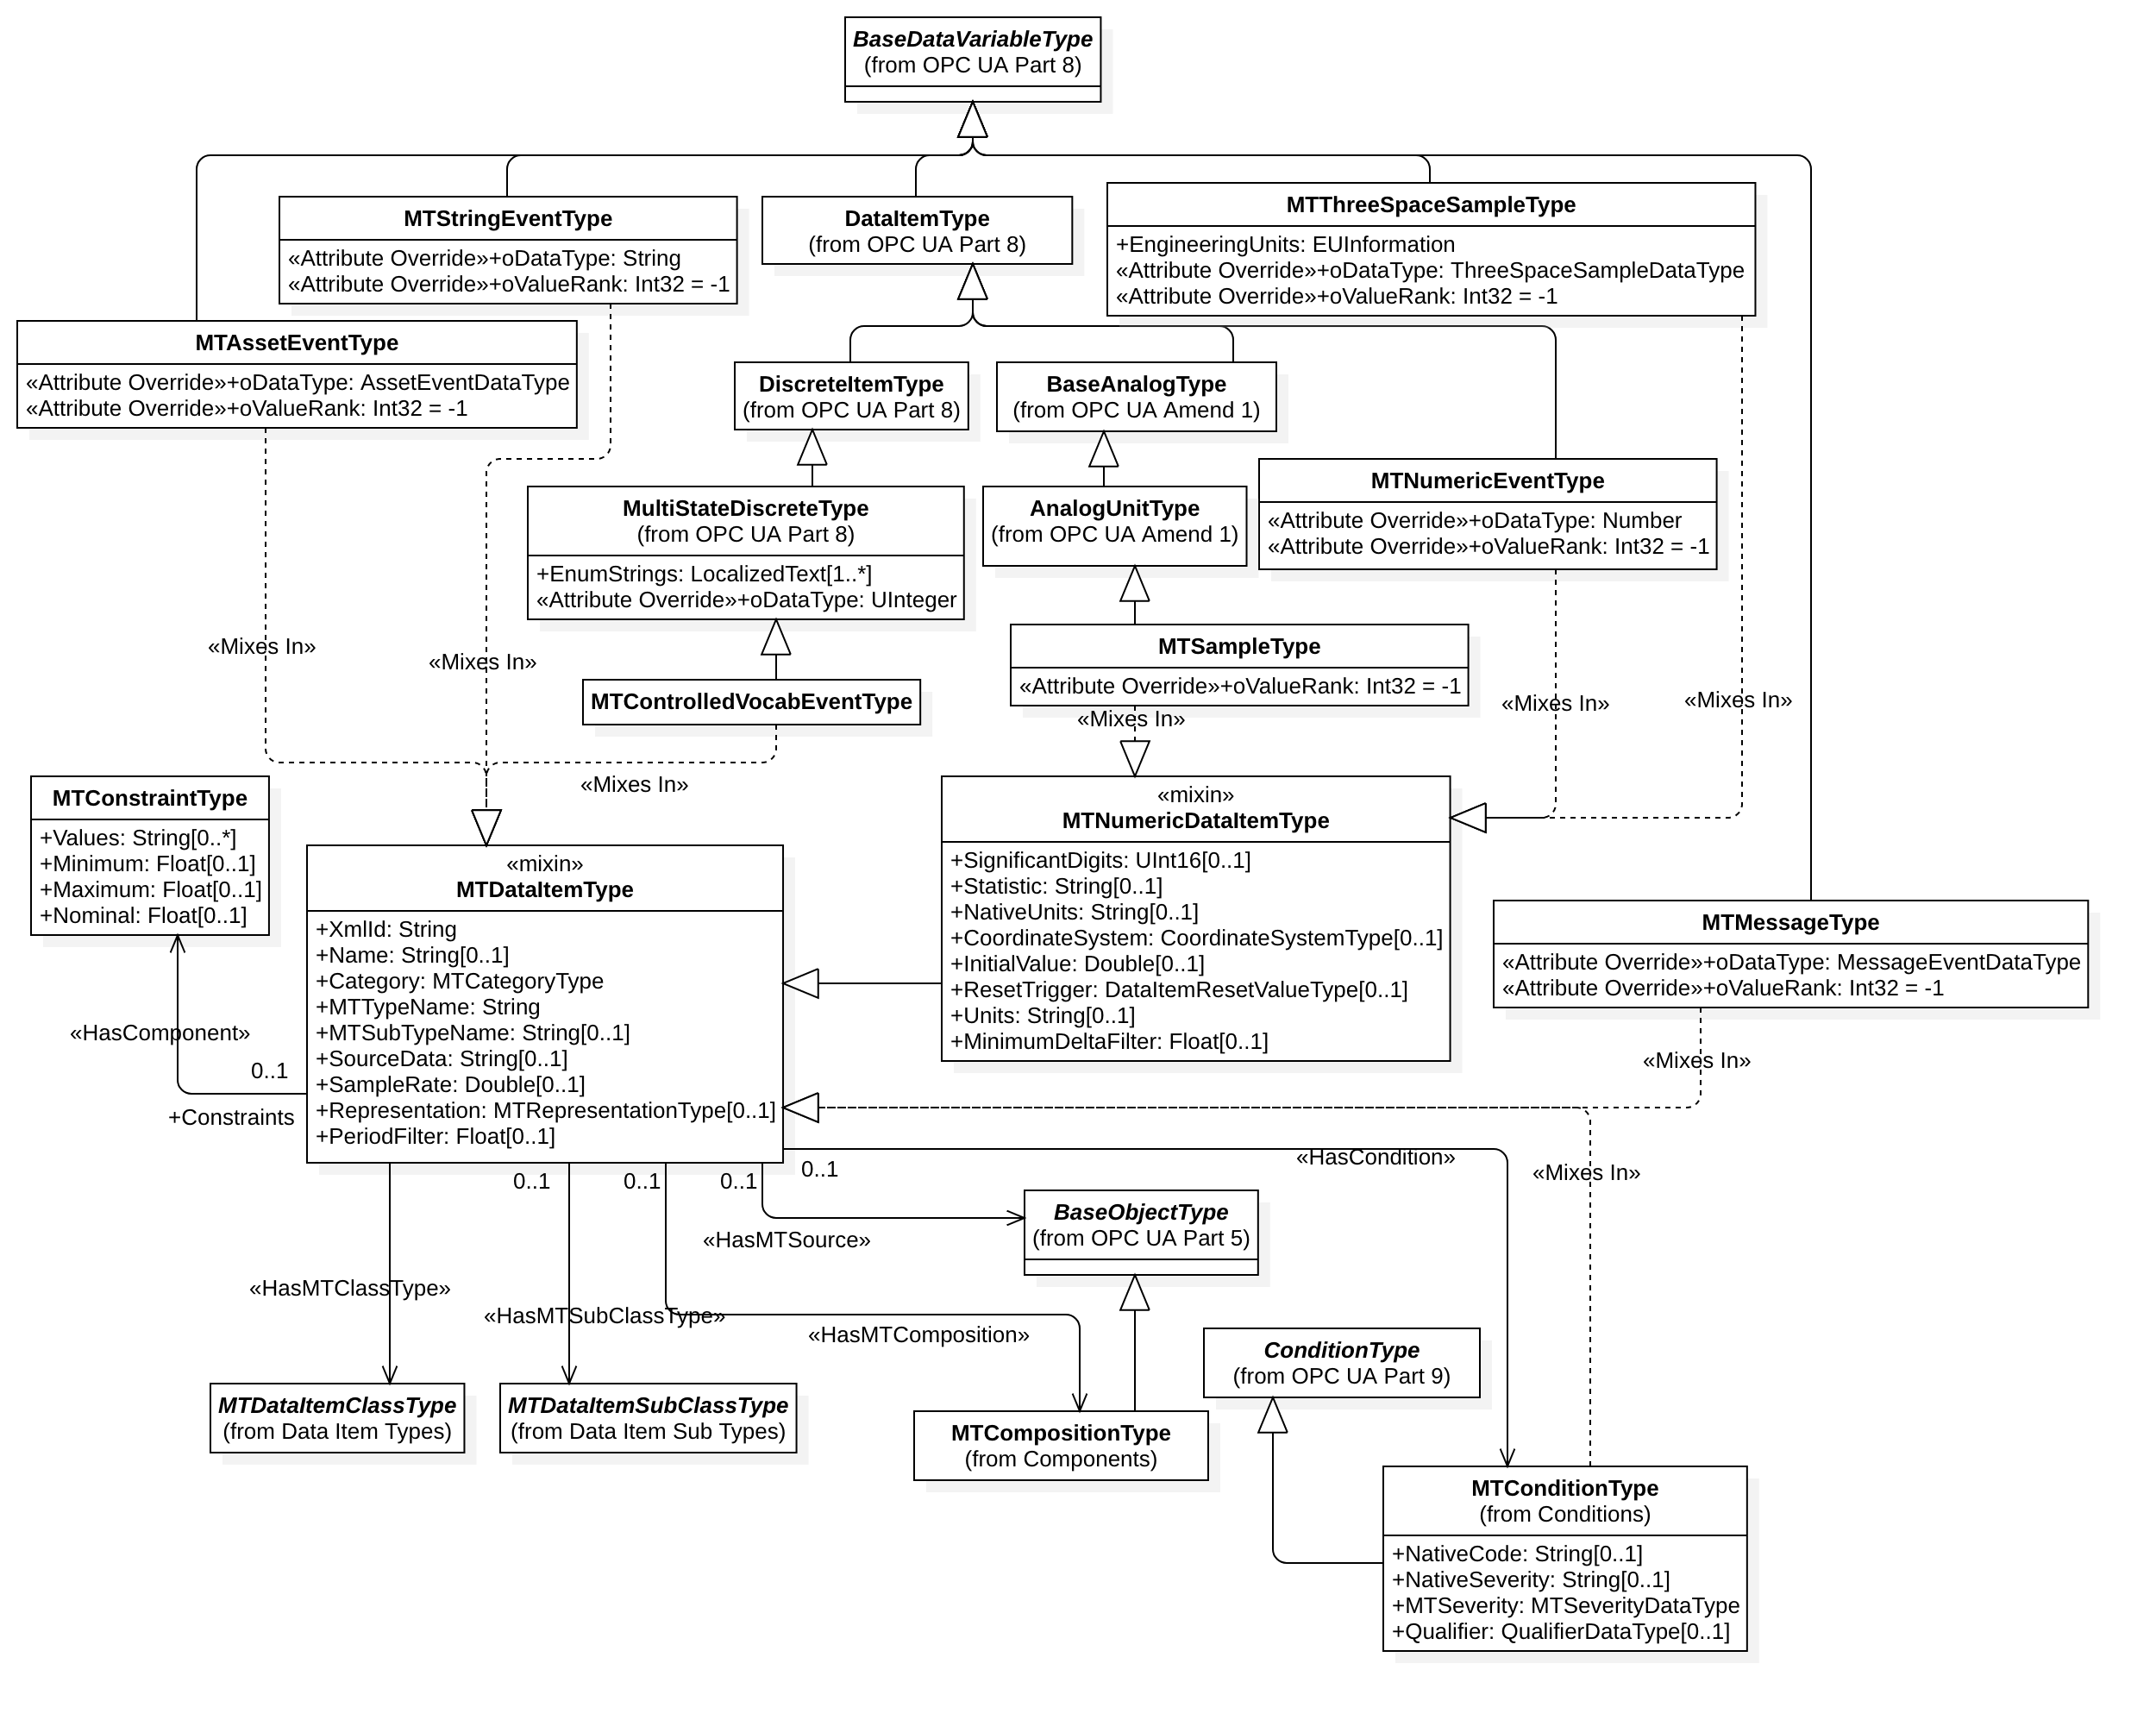
\includegraphics[width=1.0\textwidth]{./diagrams/types/DataItems.png}
  \caption{Data Items Diagram}
  \label{fig:DataItems}
\end{figure}

\FloatBarrier


\input ./type-sections/DataItems.tex

\subsubsection{Defintion of \texttt{ AssetEventDataType}}
  \label{type:AssetEventDataType}

\FloatBarrier

A special \gls{Variable} data type for asset change with a \mtmodel{AssetType} and \mtmodel{AssetId}.

\begin{table}[ht]
\centering 
  \caption{\texttt{AssetEventDataType} DataType}
  \label{data-type:AssetEventDataType}
\tabulinesep=3pt
\begin{tabu} to 6in {|l|l|} \everyrow{\hline}
\hline
\rowfont\bfseries {Field} & {Type}  \\
\tabucline[1.5pt]{}
\texttt{AssetId} & \texttt{String} \\
\texttt{AssetType} & \texttt{String} \\
\end{tabu}
\end{table} 

\FloatBarrier
\subsubsection{Defintion of \texttt{ MTAssetEventType}}
  \label{type:MTAssetEventType}

\FloatBarrier

The asset events have an additional attribute regarding the asset change or removal identifier
and the type of asset that is being reported.


\begin{table}[ht]
\centering 
  \caption{\texttt{MTAssetEventType} Definition}
  \label{table:MTAssetEventType}
\fontsize{9pt}{11pt}\selectfont
\tabulinesep=3pt
\begin{tabu} to 6in {|X[-1.35]|X[-0.7]|X[-1.75]|X[-1.5]|X[-1]|X[-0.7]|} \everyrow{\hline}
\hline
\rowfont\bfseries {Attribute} & \multicolumn{5}{|l|}{Value} \\
\tabucline[1.5pt]{}
BrowseName & \multicolumn{5}{|l|}{MTAssetEventType} \\
IsAbstract & \multicolumn{5}{|l|}{False} \\
ValueRank & \multicolumn{5}{|l|}{-1} \\
DataType & \multicolumn{5}{|l|}{AssetEventDataType} \\
\tabucline[1.5pt]{}
\rowfont \bfseries References & NodeClass & BrowseName & DataType & Type\-Definition & {Modeling\-Rule} \\
\multicolumn{6}{|l|}{Subtype of BaseDataVariableType (See \cite{UAPart8} Documentation)} \\
Has\-Property & Variable & Xml\-Id & String & Property\-Type & Mandatory \\
Has\-Property & Variable & Name & String & Property\-Type & Optional \\
Has\-Property & Variable & Category & MT\-Category\-Type & Property\-Type & Mandatory \\
Has\-Property & Variable & MT\-Type\-Name & String & Property\-Type & Mandatory \\
Has\-Property & Variable & MT\-Sub\-Type\-Name & String & Property\-Type & Optional \\
Has\-Property & Variable & Source\-Data & String & Property\-Type & Optional \\
Has\-Property & Variable & Sample\-Rate & Double & Property\-Type & Optional \\
Has\-Property & Variable & Representation & MT\-Representation\-Type & Property\-Type & Optional \\
Has\-Property & Variable & Period\-Filter & Float & Property\-Type & Optional \\
Has\-MT\-Class\-Type & Object & <MT\-Data\-Item\-Class> & \multicolumn{2}{l|}{MTDataItemClassType} & Mandatory \\
Has\-MT\-Sub\-Class\-Type & Object & <MT\-Data\-Item\-Sub\-Class> & \multicolumn{2}{l|}{MTDataItemSubClassType} & Optional \\
Has\-MT\-Composition & Object & <MT\-Composition> & \multicolumn{2}{l|}{MTCompositionType} & Optional \\
Has\-MT\-Source & Object & <Base\-Object> & \multicolumn{2}{l|}{BaseObjectType} & Optional \\
Has\-Condition & Event & <MT\-Condition> & \multicolumn{2}{l|}{MTConditionType} & Optional \\
Has\-Component & Object & Constraints & \multicolumn{2}{l|}{MTConstraintType} & Optional \\
\end{tabu}
\end{table} 


\paragraph{Dependencies and Relationships}

\begin{itemize}
\item Mixes in \texttt{MTDataItemType}, see See section \ref{type:MTDataItemType}
\end{itemize}
\FloatBarrier
\subsubsection{Defintion of \texttt{ MTConditionClassType}}
  \label{type:MTConditionClassType}

\FloatBarrier

The abstract type for all data items types that are specifically for \mtmodel{CONDITION} \gls{category}.

\begin{table}[ht]
\centering 
  \caption{\texttt{MTConditionClassType} Definition}
  \label{table:MTConditionClassType}
\fontsize{9pt}{11pt}\selectfont
\tabulinesep=3pt
\begin{tabu} to 6in {|X[-1.35]|X[-0.7]|X[-1.75]|X[-1.5]|X[-1]|X[-0.7]|} \everyrow{\hline}
\hline
\rowfont\bfseries {Attribute} & \multicolumn{5}{|l|}{Value} \\
\tabucline[1.5pt]{}
BrowseName & \multicolumn{5}{|l|}{MTConditionClassType} \\
IsAbstract & \multicolumn{5}{|l|}{True} \\
\tabucline[1.5pt]{}
\rowfont \bfseries References & NodeClass & BrowseName & DataType & Type\-Definition & {Modeling\-Rule} \\
\multicolumn{6}{|l|}{Subtype of MTDataItemClassType (See Data Item Types Documentation)} \\
HasSubtype & ObjectType & \multicolumn{2}{l}{ActuatorClassType} & \multicolumn{2}{|l|}{See section \ref{type:ActuatorClassType}} \\
HasSubtype & ObjectType & \multicolumn{2}{l}{CommunicationsClassType} & \multicolumn{2}{|l|}{See section \ref{type:CommunicationsClassType}} \\
HasSubtype & ObjectType & \multicolumn{2}{l}{DataRangeClassType} & \multicolumn{2}{|l|}{See section \ref{type:DataRangeClassType}} \\
HasSubtype & ObjectType & \multicolumn{2}{l}{LogicProgramClassType} & \multicolumn{2}{|l|}{See section \ref{type:LogicProgramClassType}} \\
HasSubtype & ObjectType & \multicolumn{2}{l}{HardwareClassType} & \multicolumn{2}{|l|}{See section \ref{type:HardwareClassType}} \\
HasSubtype & ObjectType & \multicolumn{2}{l}{MotionProgramClassType} & \multicolumn{2}{|l|}{See section \ref{type:MotionProgramClassType}} \\
HasSubtype & ObjectType & \multicolumn{2}{l}{SystemClassType} & \multicolumn{2}{|l|}{See section \ref{type:SystemClassType}} \\
\end{tabu}
\end{table} 


\FloatBarrier
\subsubsection{Defintion of \texttt{ MTConstraintType}}
  \label{type:MTConstraintType}

\FloatBarrier

The MTConnect constraints. The Values or the Minimum, Maximum, and Nominal values should be 
provided. Multiple Values can be provided as an array as a set of allowable values for this
\gls{MTDataItem}.

\begin{table}[ht]
\centering 
  \caption{\texttt{MTConstraintType} Definition}
  \label{table:MTConstraintType}
\fontsize{9pt}{11pt}\selectfont
\tabulinesep=3pt
\begin{tabu} to 6in {|X[-1.35]|X[-0.7]|X[-1.75]|X[-1.5]|X[-1]|X[-0.7]|} \everyrow{\hline}
\hline
\rowfont\bfseries {Attribute} & \multicolumn{5}{|l|}{Value} \\
\tabucline[1.5pt]{}
BrowseName & \multicolumn{5}{|l|}{MTConstraintType} \\
IsAbstract & \multicolumn{5}{|l|}{False} \\
\tabucline[1.5pt]{}
\rowfont \bfseries References & NodeClass & BrowseName & DataType & Type\-Definition & {Modeling\-Rule} \\
\multicolumn{6}{|l|}{Subtype of BaseObjectType (See \cite{UAPart5} Documentation)} \\
Has\-Property & Variable & Values & String[] & Property\-Type & Optional \\
Has\-Property & Variable & Minimum & Float & Property\-Type & Optional \\
Has\-Property & Variable & Maximum & Float & Property\-Type & Optional \\
Has\-Property & Variable & Nominal & Float & Property\-Type & Optional \\
\end{tabu}
\end{table} 


\FloatBarrier
\subsubsection{Defintion of \texttt{ MTControlledVocabEventType}}
  \label{type:MTControlledVocabEventType}

\FloatBarrier

All \glspl{MTDataItem} with \gls{category} \mtmodel{EVENT} having Controlled Vocabularies (Enumerations) 
will be added as sub-types of this type which is mapped to the OPC/UA MultiStateValueDiscreteType. 
Otherwise, either \mtmodel{MTString} or \mtmodel{MTNumeric} will be used. All subtypes are direct representations of the 
MTConnect equivalent elements that can be found in the MTConnect Part 3 \cite{MTCPart3} documents.

\begin{table}[ht]
\centering 
  \caption{\texttt{MTControlledVocabEventType} Definition}
  \label{table:MTControlledVocabEventType}
\fontsize{9pt}{11pt}\selectfont
\tabulinesep=3pt
\begin{tabu} to 6in {|X[-1.35]|X[-0.7]|X[-1.75]|X[-1.5]|X[-1]|X[-0.7]|} \everyrow{\hline}
\hline
\rowfont\bfseries {Attribute} & \multicolumn{5}{|l|}{Value} \\
\tabucline[1.5pt]{}
BrowseName & \multicolumn{5}{|l|}{MTControlledVocabEventType} \\
IsAbstract & \multicolumn{5}{|l|}{False} \\
ValueRank & \multicolumn{5}{|l|}{-2} \\
DataType & \multicolumn{5}{|l|}{UInteger} \\
\tabucline[1.5pt]{}
\rowfont \bfseries References & NodeClass & BrowseName & DataType & Type\-Definition & {Modeling\-Rule} \\
\multicolumn{6}{|l|}{Subtype of MultiStateDiscreteType (See \cite{UAPart8} Documentation)} \\
Has\-Property & Variable & Xml\-Id & String & Property\-Type & Mandatory \\
Has\-Property & Variable & Name & String & Property\-Type & Optional \\
Has\-Property & Variable & Category & MT\-Category\-Type & Property\-Type & Mandatory \\
Has\-Property & Variable & MT\-Type\-Name & String & Property\-Type & Mandatory \\
Has\-Property & Variable & MT\-Sub\-Type\-Name & String & Property\-Type & Optional \\
Has\-Property & Variable & Source\-Data & String & Property\-Type & Optional \\
Has\-Property & Variable & Sample\-Rate & Double & Property\-Type & Optional \\
Has\-Property & Variable & Representation & MT\-Representation\-Type & Property\-Type & Optional \\
Has\-Property & Variable & Period\-Filter & Float & Property\-Type & Optional \\
Has\-MT\-Class\-Type & Object & <MT\-Data\-Item\-Class> & \multicolumn{2}{l|}{MTDataItemClassType} & Mandatory \\
Has\-MT\-Sub\-Class\-Type & Object & <MT\-Data\-Item\-Sub\-Class> & \multicolumn{2}{l|}{MTDataItemSubClassType} & Optional \\
Has\-MT\-Composition & Object & <MT\-Composition> & \multicolumn{2}{l|}{MTCompositionType} & Optional \\
Has\-MT\-Source & Object & <Base\-Object> & \multicolumn{2}{l|}{BaseObjectType} & Optional \\
Has\-Condition & Event & <MT\-Condition> & \multicolumn{2}{l|}{MTConditionType} & Optional \\
Has\-Component & Object & Constraints & \multicolumn{2}{l|}{MTConstraintType} & Optional \\
\end{tabu}
\end{table} 


\paragraph{Dependencies and Relationships}

\begin{itemize}
\item Mixes in \texttt{MTDataItemType}, see See section \ref{type:MTDataItemType}
\end{itemize}
\FloatBarrier
\subsubsection{Defintion of \texttt{<<mixin>> MTDataItemType}}
  \label{type:MTDataItemType}

\FloatBarrier

The data item mixin will inject the properties and the methods into the related 
classes. This facility is similar to the Ruby module mixin or the Scala traits.

\begin{table}[ht]
\centering 
  \caption{\texttt{MTDataItemType} Definition}
  \label{table:MTDataItemType}
\fontsize{9pt}{11pt}\selectfont
\tabulinesep=3pt
\begin{tabu} to 6in {|X[-1.35]|X[-0.7]|X[-1.75]|X[-1.5]|X[-1]|X[-0.7]|} \everyrow{\hline}
\hline
\rowfont\bfseries {Attribute} & \multicolumn{5}{|l|}{Value} \\
\tabucline[1.5pt]{}
BrowseName & \multicolumn{5}{|l|}{MTDataItemType} \\
IsAbstract & \multicolumn{5}{|l|}{False} \\
\tabucline[1.5pt]{}
\rowfont \bfseries References & NodeClass & BrowseName & DataType & Type\-Definition & {Modeling\-Rule} \\
HasSubtype & ObjectType & \multicolumn{2}{l}{MTNumericDataItemType} & \multicolumn{2}{|l|}{See section \ref{type:MTNumericDataItemType}} \\
Has\-Property & Variable & Xml\-Id & String & Property\-Type & Mandatory \\
Has\-Property & Variable & Name & String & Property\-Type & Optional \\
Has\-Property & Variable & Category & MT\-Category\-Type & Property\-Type & Mandatory \\
Has\-Property & Variable & MT\-Type\-Name & String & Property\-Type & Mandatory \\
Has\-Property & Variable & MT\-Sub\-Type\-Name & String & Property\-Type & Optional \\
Has\-Property & Variable & Source\-Data & String & Property\-Type & Optional \\
Has\-Property & Variable & Sample\-Rate & Double & Property\-Type & Optional \\
Has\-Property & Variable & Representation & MT\-Representation\-Type & Property\-Type & Optional \\
Has\-Property & Variable & Period\-Filter & Float & Property\-Type & Optional \\
Has\-MT\-Class\-Type & Object & <MT\-Data\-Item\-Class> & \multicolumn{2}{l|}{MTDataItemClassType} & Mandatory \\
Has\-MT\-Sub\-Class\-Type & Object & <MT\-Data\-Item\-Sub\-Class> & \multicolumn{2}{l|}{MTDataItemSubClassType} & Optional \\
Has\-MT\-Composition & Object & <MT\-Composition> & \multicolumn{2}{l|}{MTCompositionType} & Optional \\
Has\-MT\-Source & Object & <Base\-Object> & \multicolumn{2}{l|}{BaseObjectType} & Optional \\
Has\-Condition & Event & <MT\-Condition> & \multicolumn{2}{l|}{MTConditionType} & Optional \\
Has\-Component & Object & Constraints & \multicolumn{2}{l|}{MTConstraintType} & Optional \\
\end{tabu}
\end{table} 


\FloatBarrier
\paragraph{Referenced Properties and Objects}

\begin{itemize}
\item \textbf{Allowable Values} for \texttt{MTCategoryType}
\FloatBarrier

Represents the \gls{category} attribute of the MTConnect \gls{MTDataItem}.

\begin{table}[ht]
\centering 
  \caption{\texttt{MTCategoryType} Enumeration}
  \label{enum:MTCategoryType}
\tabulinesep=3pt
\begin{tabu} to 6in {|l|r|} \everyrow{\hline}
\hline
\rowfont\bfseries {Name} & {Index} \\
\tabucline[1.5pt]{}
\texttt{EVENT} & \texttt{0} \\
\texttt{CONDITION} & \texttt{1} \\
\texttt{SAMPLE} & \texttt{2} \\
\end{tabu}
\end{table} 
\FloatBarrier
\item \texttt{SourceData::String:} The text that is the \gls{CDATA} of the \mtmodel{Source} element.

\item \textbf{Allowable Values} for \texttt{MTRepresentationType}
\FloatBarrier

Represents the \mtmodel{representation} attribute of the MTConnect \gls{MTDataItem}.

\begin{table}[ht]
\centering 
  \caption{\texttt{MTRepresentationType} Enumeration}
  \label{enum:MTRepresentationType}
\tabulinesep=3pt
\begin{tabu} to 6in {|l|r|} \everyrow{\hline}
\hline
\rowfont\bfseries {Name} & {Index} \\
\tabucline[1.5pt]{}
\texttt{DISCRETE} & \texttt{0} \\
\texttt{TIME_SERIES} & \texttt{1} \\
\texttt{VALUE} & \texttt{2} \\
\end{tabu}
\end{table} 
\FloatBarrier
\item \texttt{PeriodFilter::Float:} Represents the MTConnect \mtmodel{Filter} subtype of \mtmodel{PeriodFilter}.

\item \textbf{Allowable Values} for \texttt{MTRepresentationType}
\FloatBarrier

Represents the \mtmodel{representation} attribute of the MTConnect \gls{MTDataItem}.

\begin{table}[ht]
\centering 
  \caption{\texttt{MTRepresentationType} Enumeration}
\tabulinesep=3pt
\begin{tabu} to 6in {|l|r|} \everyrow{\hline}
\hline
\rowfont\bfseries {Name} & {Index} \\
\tabucline[1.5pt]{}
\texttt{DISCRETE} & \texttt{0} \\
\texttt{TIME_SERIES} & \texttt{1} \\
\texttt{VALUE} & \texttt{2} \\
\end{tabu}
\end{table} 
\FloatBarrier
\item \textbf{Allowable Values} for \texttt{MTCategoryType}
\FloatBarrier

Represents the \gls{category} attribute of the MTConnect \gls{MTDataItem}.

\begin{table}[ht]
\centering 
  \caption{\texttt{MTCategoryType} Enumeration}
\tabulinesep=3pt
\begin{tabu} to 6in {|l|r|} \everyrow{\hline}
\hline
\rowfont\bfseries {Name} & {Index} \\
\tabucline[1.5pt]{}
\texttt{EVENT} & \texttt{0} \\
\texttt{CONDITION} & \texttt{1} \\
\texttt{SAMPLE} & \texttt{2} \\
\end{tabu}
\end{table} 
\FloatBarrier
\end{itemize}
\paragraph{Operations}
\begin{itemize}
  \item \texttt{getStatusCode()}
    Documentation: The OPC UA status code will be created using the following process:

\begin{itemize}
  \item If the value of the data item is \mtmodel{UNAVAILABLE} a status code of \uamodel{Uncertain_NoCommunicationLastUsable}
  \item When a reset trigger is specified, new \uamodel{Good_} status codes will be created. See \mtmodel{ResetTrigger} enumeration.
\end{itemize}

\end{itemize}
\paragraph{Dependencies and Relationships}

\begin{itemize}
\item \textbf{Allowable Values} for \texttt{MTRepresentationType}
\FloatBarrier

Represents the \mtmodel{representation} attribute of the MTConnect \gls{MTDataItem}.

\begin{table}[ht]
\centering 
  \caption{\texttt{MTRepresentationType} Enumeration}
\tabulinesep=3pt
\begin{tabu} to 6in {|l|r|} \everyrow{\hline}
\hline
\rowfont\bfseries {Name} & {Index} \\
\tabucline[1.5pt]{}
\texttt{DISCRETE} & \texttt{0} \\
\texttt{TIME_SERIES} & \texttt{1} \\
\texttt{VALUE} & \texttt{2} \\
\end{tabu}
\end{table} 
\FloatBarrier
\item \textbf{Allowable Values} for \texttt{MTCategoryType}
\FloatBarrier

Represents the \gls{category} attribute of the MTConnect \gls{MTDataItem}.

\begin{table}[ht]
\centering 
  \caption{\texttt{MTCategoryType} Enumeration}
\tabulinesep=3pt
\begin{tabu} to 6in {|l|r|} \everyrow{\hline}
\hline
\rowfont\bfseries {Name} & {Index} \\
\tabucline[1.5pt]{}
\texttt{EVENT} & \texttt{0} \\
\texttt{CONDITION} & \texttt{1} \\
\texttt{SAMPLE} & \texttt{2} \\
\end{tabu}
\end{table} 
\FloatBarrier
\end{itemize}
\FloatBarrier
\subsubsection{Defintion of \texttt{<<mixin>> MTNumericDataItemType}}
  \label{type:MTNumericDataItemType}

\FloatBarrier

These are the additional attributes that are relevent to numeric data items. 
The factory will evaluate these values and will set the engineering units and the 
range associated with the parent entity.

\begin{table}[ht]
\centering 
  \caption{\texttt{MTNumericDataItemType} Definition}
  \label{table:MTNumericDataItemType}
\fontsize{9pt}{11pt}\selectfont
\tabulinesep=3pt
\begin{tabu} to 6in {|X[-1.35]|X[-0.7]|X[-1.75]|X[-1.5]|X[-1]|X[-0.7]|} \everyrow{\hline}
\hline
\rowfont\bfseries {Attribute} & \multicolumn{5}{|l|}{Value} \\
\tabucline[1.5pt]{}
BrowseName & \multicolumn{5}{|l|}{MTNumericDataItemType} \\
IsAbstract & \multicolumn{5}{|l|}{False} \\
\tabucline[1.5pt]{}
\rowfont \bfseries References & NodeClass & BrowseName & DataType & Type\-Definition & {Modeling\-Rule} \\
\multicolumn{6}{|l|}{Subtype of MTDataItemType (See section \ref{type:MTDataItemType})} \\
Has\-Property & Variable & Significant\-Digits & UInt16 & Property\-Type & Optional \\
Has\-Property & Variable & Statistic & String & Property\-Type & Optional \\
Has\-Property & Variable & Native\-Units & String & Property\-Type & Optional \\
Has\-Property & Variable & Coordinate\-System & Coordinate\-System\-Type & Property\-Type & Optional \\
Has\-Property & Variable & Initial\-Value & Double & Property\-Type & Optional \\
Has\-Property & Variable & Reset\-Trigger & Data\-Item\-Reset\-Value\-Type & Property\-Type & Optional \\
Has\-Property & Variable & Units & String & Property\-Type & Optional \\
Has\-Property & Variable & Minimum\-Delta\-Filter & Float & Property\-Type & Optional \\
\end{tabu}
\end{table} 


\FloatBarrier
\paragraph{Referenced Properties and Objects}

\begin{itemize}
\item \texttt{SignificantDigits::UInt16:} The significant digits is converted to a \uaterm{ValuePrecision}.

\item \textbf{Allowable Values} for \texttt{CoordinateSystemType}
\FloatBarrier

Represents the \mtmodel{coordinateSystem} attribute of the MTConnect \gls{MTDataItem}.

\begin{table}[ht]
\centering 
  \caption{\texttt{CoordinateSystemType} Enumeration}
  \label{enum:CoordinateSystemType}
\tabulinesep=3pt
\begin{tabu} to 6in {|l|r|} \everyrow{\hline}
\hline
\rowfont\bfseries {Name} & {Index} \\
\tabucline[1.5pt]{}
\texttt{MACHINE} & \texttt{0} \\
\texttt{WORK} & \texttt{1} \\
\end{tabu}
\end{table} 
\FloatBarrier
\item \textbf{Allowable Values} for \texttt{DataItemResetValueType}
\FloatBarrier

These need to become \uamodel{Good_} status code in OPC UA.

\begin{table}[ht]
\centering 
  \caption{\texttt{DataItemResetValueType} Enumeration}
  \label{enum:DataItemResetValueType}
\tabulinesep=3pt
\begin{tabu} to 6in {|l|r|} \everyrow{\hline}
\hline
\rowfont\bfseries {Name} & {Index} \\
\tabucline[1.5pt]{}
\texttt{ACTION_COMPLETE} & \texttt{0} \\
\texttt{ANNUAL} & \texttt{1} \\
\texttt{DAY} & \texttt{2} \\
\texttt{MAINTENANCE} & \texttt{3} \\
\texttt{MANUAL} & \texttt{4} \\
\texttt{MONTH} & \texttt{5} \\
\texttt{POWER_ON} & \texttt{6} \\
\texttt{SHIFT} & \texttt{7} \\
\texttt{WEEK} & \texttt{8} \\
\end{tabu}
\end{table} 
\FloatBarrier
\item \texttt{MinimumDeltaFilter::Float:} Represents the MTConnect \mtmodel{Filter} subtype of \mtmodel{MinimumDeltaFilter}.

\item \textbf{Allowable Values} for \texttt{CoordinateSystemType}
\FloatBarrier

Represents the \mtmodel{coordinateSystem} attribute of the MTConnect \gls{MTDataItem}.

\begin{table}[ht]
\centering 
  \caption{\texttt{CoordinateSystemType} Enumeration}
\tabulinesep=3pt
\begin{tabu} to 6in {|l|r|} \everyrow{\hline}
\hline
\rowfont\bfseries {Name} & {Index} \\
\tabucline[1.5pt]{}
\texttt{MACHINE} & \texttt{0} \\
\texttt{WORK} & \texttt{1} \\
\end{tabu}
\end{table} 
\FloatBarrier
\item \textbf{Allowable Values} for \texttt{DataItemResetValueType}
\FloatBarrier

These need to become \uamodel{Good_} status code in OPC UA.

\begin{table}[ht]
\centering 
  \caption{\texttt{DataItemResetValueType} Enumeration}
\tabulinesep=3pt
\begin{tabu} to 6in {|l|r|} \everyrow{\hline}
\hline
\rowfont\bfseries {Name} & {Index} \\
\tabucline[1.5pt]{}
\texttt{ACTION_COMPLETE} & \texttt{0} \\
\texttt{ANNUAL} & \texttt{1} \\
\texttt{DAY} & \texttt{2} \\
\texttt{MAINTENANCE} & \texttt{3} \\
\texttt{MANUAL} & \texttt{4} \\
\texttt{MONTH} & \texttt{5} \\
\texttt{POWER_ON} & \texttt{6} \\
\texttt{SHIFT} & \texttt{7} \\
\texttt{WEEK} & \texttt{8} \\
\end{tabu}
\end{table} 
\FloatBarrier
\end{itemize}
\paragraph{Dependencies and Relationships}

\begin{itemize}
\item \textbf{Allowable Values} for \texttt{CoordinateSystemType}
\FloatBarrier

Represents the \mtmodel{coordinateSystem} attribute of the MTConnect \gls{MTDataItem}.

\begin{table}[ht]
\centering 
  \caption{\texttt{CoordinateSystemType} Enumeration}
\tabulinesep=3pt
\begin{tabu} to 6in {|l|r|} \everyrow{\hline}
\hline
\rowfont\bfseries {Name} & {Index} \\
\tabucline[1.5pt]{}
\texttt{MACHINE} & \texttt{0} \\
\texttt{WORK} & \texttt{1} \\
\end{tabu}
\end{table} 
\FloatBarrier
\item \textbf{Allowable Values} for \texttt{DataItemResetValueType}
\FloatBarrier

These need to become \uamodel{Good_} status code in OPC UA.

\begin{table}[ht]
\centering 
  \caption{\texttt{DataItemResetValueType} Enumeration}
\tabulinesep=3pt
\begin{tabu} to 6in {|l|r|} \everyrow{\hline}
\hline
\rowfont\bfseries {Name} & {Index} \\
\tabucline[1.5pt]{}
\texttt{ACTION_COMPLETE} & \texttt{0} \\
\texttt{ANNUAL} & \texttt{1} \\
\texttt{DAY} & \texttt{2} \\
\texttt{MAINTENANCE} & \texttt{3} \\
\texttt{MANUAL} & \texttt{4} \\
\texttt{MONTH} & \texttt{5} \\
\texttt{POWER_ON} & \texttt{6} \\
\texttt{SHIFT} & \texttt{7} \\
\texttt{WEEK} & \texttt{8} \\
\end{tabu}
\end{table} 
\FloatBarrier
\end{itemize}
\FloatBarrier
\subsubsection{Defintion of \texttt{ MTEventClassType}}
  \label{type:MTEventClassType}

\FloatBarrier

The base type class for all data items with a \gls{category} of \mtmodel{EVENT}.

\begin{table}[ht]
\centering 
  \caption{\texttt{MTEventClassType} Definition}
  \label{table:MTEventClassType}
\fontsize{9pt}{11pt}\selectfont
\tabulinesep=3pt
\begin{tabu} to 6in {|X[-1.35]|X[-0.7]|X[-1.75]|X[-1.5]|X[-1]|X[-0.7]|} \everyrow{\hline}
\hline
\rowfont\bfseries {Attribute} & \multicolumn{5}{|l|}{Value} \\
\tabucline[1.5pt]{}
BrowseName & \multicolumn{5}{|l|}{MTEventClassType} \\
IsAbstract & \multicolumn{5}{|l|}{True} \\
\tabucline[1.5pt]{}
\rowfont \bfseries References & NodeClass & BrowseName & DataType & Type\-Definition & {Modeling\-Rule} \\
\multicolumn{6}{|l|}{Subtype of MTDataItemClassType (See Data Item Types Documentation)} \\
HasSubtype & ObjectType & \multicolumn{2}{l}{MTControlledVocabClassType} & \multicolumn{2}{|l|}{See section \ref{type:MTControlledVocabClassType}} \\
HasSubtype & ObjectType & \multicolumn{2}{l}{MTNumericEventClassType} & \multicolumn{2}{|l|}{See section \ref{type:MTNumericEventClassType}} \\
HasSubtype & ObjectType & \multicolumn{2}{l}{MTStringEventClassType} & \multicolumn{2}{|l|}{See section \ref{type:MTStringEventClassType}} \\
HasSubtype & ObjectType & \multicolumn{2}{l}{MTMessageClassType} & \multicolumn{2}{|l|}{See section \ref{type:MTMessageClassType}} \\
\end{tabu}
\end{table} 


\FloatBarrier
\subsubsection{Defintion of \texttt{ MTMessageType}}
  \label{type:MTMessageType}

\FloatBarrier

The message type is a special class since it adds another property for the \mtmodel{nativeCode}. 
In MTConnect the \mtmodel{nativeCode} attribute will be mapped to this variable 
in the message. The type is currently sub-typed from the OPC UA \uamodel{SystemEventType} and 
will be represented as an event. The MTConnect \gls{CDATA} will be represented in the \gls{MTEvent}
\mtmodel{Message}.


\begin{table}[ht]
\centering 
  \caption{\texttt{MTMessageType} Definition}
  \label{table:MTMessageType}
\fontsize{9pt}{11pt}\selectfont
\tabulinesep=3pt
\begin{tabu} to 6in {|X[-1.35]|X[-0.7]|X[-1.75]|X[-1.5]|X[-1]|X[-0.7]|} \everyrow{\hline}
\hline
\rowfont\bfseries {Attribute} & \multicolumn{5}{|l|}{Value} \\
\tabucline[1.5pt]{}
BrowseName & \multicolumn{5}{|l|}{MTMessageType} \\
IsAbstract & \multicolumn{5}{|l|}{False} \\
\tabucline[1.5pt]{}
\rowfont \bfseries References & NodeClass & BrowseName & DataType & Type\-Definition & {Modeling\-Rule} \\
\multicolumn{6}{|l|}{Subtype of SystemEventType (See \cite{UAPart5} Documentation)} \\
Has\-Property & Variable & Xml\-Id & String & Property\-Type & Mandatory \\
Has\-Property & Variable & Name & String & Property\-Type & Optional \\
Has\-Property & Variable & Category & MT\-Category\-Type & Property\-Type & Mandatory \\
Has\-Property & Variable & MT\-Type\-Name & String & Property\-Type & Mandatory \\
Has\-Property & Variable & MT\-Sub\-Type\-Name & String & Property\-Type & Optional \\
Has\-Property & Variable & Source\-Data & String & Property\-Type & Optional \\
Has\-Property & Variable & Sample\-Rate & Double & Property\-Type & Optional \\
Has\-Property & Variable & Representation & MT\-Representation\-Type & Property\-Type & Optional \\
Has\-Property & Variable & Period\-Filter & Float & Property\-Type & Optional \\
Has\-MT\-Class\-Type & Object & <MT\-Data\-Item\-Class> & \multicolumn{2}{l|}{MTDataItemClassType} & Mandatory \\
Has\-MT\-Sub\-Class\-Type & Object & <MT\-Data\-Item\-Sub\-Class> & \multicolumn{2}{l|}{MTDataItemSubClassType} & Optional \\
Has\-MT\-Composition & Object & <MT\-Composition> & \multicolumn{2}{l|}{MTCompositionType} & Optional \\
Has\-MT\-Source & Object & <Base\-Object> & \multicolumn{2}{l|}{BaseObjectType} & Optional \\
Has\-Condition & Event & <MT\-Condition> & \multicolumn{2}{l|}{MTConditionType} & Optional \\
Has\-Component & Object & Constraints & \multicolumn{2}{l|}{MTConstraintType} & Optional \\
Has\-Property & Variable & Native\-Code & String & Property\-Type & Optional \\
\end{tabu}
\end{table} 


\paragraph{Dependencies and Relationships}

\begin{itemize}
\item Mixes in \texttt{MTDataItemType}, see See section \ref{type:MTDataItemType}
\end{itemize}
\FloatBarrier
\subsubsection{Defintion of \texttt{ MTNumericEventType}}
  \label{type:MTNumericEventType}

\FloatBarrier

All data items with category \gls{MTEvent} and a numeric value. These are usually counters for 
parts and lines. Currently only builtin types that are known to be integers will be
sub-typed from this type. Extended types will be subtyped from the \mtuatype{MTStringEventType}.

\begin{table}[ht]
\centering 
  \caption{\texttt{MTNumericEventType} Definition}
  \label{table:MTNumericEventType}
\fontsize{9pt}{11pt}\selectfont
\tabulinesep=3pt
\begin{tabu} to 6in {|X[-1.35]|X[-0.7]|X[-1.75]|X[-1.5]|X[-1]|X[-0.7]|} \everyrow{\hline}
\hline
\rowfont\bfseries {Attribute} & \multicolumn{5}{|l|}{Value} \\
\tabucline[1.5pt]{}
BrowseName & \multicolumn{5}{|l|}{MTNumericEventType} \\
IsAbstract & \multicolumn{5}{|l|}{False} \\
ValueRank & \multicolumn{5}{|l|}{-1} \\
DataType & \multicolumn{5}{|l|}{Number} \\
\tabucline[1.5pt]{}
\rowfont \bfseries References & NodeClass & BrowseName & DataType & Type\-Definition & {Modeling\-Rule} \\
\multicolumn{6}{|l|}{Subtype of DataItemType (See \cite{UAPart8} Documentation)} \\
Has\-Property & Variable & Xml\-Id & String & Property\-Type & Mandatory \\
Has\-Property & Variable & Name & String & Property\-Type & Optional \\
Has\-Property & Variable & Category & MT\-Category\-Type & Property\-Type & Mandatory \\
Has\-Property & Variable & MT\-Type\-Name & String & Property\-Type & Mandatory \\
Has\-Property & Variable & MT\-Sub\-Type\-Name & String & Property\-Type & Optional \\
Has\-Property & Variable & Source\-Data & String & Property\-Type & Optional \\
Has\-Property & Variable & Sample\-Rate & Double & Property\-Type & Optional \\
Has\-Property & Variable & Representation & MT\-Representation\-Type & Property\-Type & Optional \\
Has\-Property & Variable & Period\-Filter & Float & Property\-Type & Optional \\
Has\-MT\-Class\-Type & Object & <MT\-Data\-Item\-Class> & \multicolumn{2}{l|}{MTDataItemClassType} & Mandatory \\
Has\-MT\-Sub\-Class\-Type & Object & <MT\-Data\-Item\-Sub\-Class> & \multicolumn{2}{l|}{MTDataItemSubClassType} & Optional \\
Has\-MT\-Composition & Object & <MT\-Composition> & \multicolumn{2}{l|}{MTCompositionType} & Optional \\
Has\-MT\-Source & Object & <Base\-Object> & \multicolumn{2}{l|}{BaseObjectType} & Optional \\
Has\-Condition & Event & <MT\-Condition> & \multicolumn{2}{l|}{MTConditionType} & Optional \\
Has\-Component & Object & Constraints & \multicolumn{2}{l|}{MTConstraintType} & Optional \\
Has\-Property & Variable & Significant\-Digits & UInt16 & Property\-Type & Optional \\
Has\-Property & Variable & Statistic & String & Property\-Type & Optional \\
Has\-Property & Variable & Native\-Units & String & Property\-Type & Optional \\
Has\-Property & Variable & Coordinate\-System & Coordinate\-System\-Type & Property\-Type & Optional \\
Has\-Property & Variable & Initial\-Value & Double & Property\-Type & Optional \\
Has\-Property & Variable & Reset\-Trigger & Data\-Item\-Reset\-Value\-Type & Property\-Type & Optional \\
Has\-Property & Variable & Units & String & Property\-Type & Optional \\
Has\-Property & Variable & Minimum\-Delta\-Filter & Float & Property\-Type & Optional \\
\end{tabu}
\end{table} 


\paragraph{Dependencies and Relationships}

\begin{itemize}
\item Mixes in \texttt{MTNumericDataItemType}, see See section \ref{type:MTNumericDataItemType}
\end{itemize}
\FloatBarrier
\subsubsection{Defintion of \texttt{ MTSampleType}}
  \label{type:MTSampleType}

\FloatBarrier

Data Items with category \mtmodel{SAMPLE}. The simplest mapping since all these types are 
floating point numeric data and comply with the \uamodel{AnalogUnitType} from \cite{UAPart8} Amendment 1.
In ammendment 1, the \uamodel{EURange} is optional. \uamodel{EngineeringUnits} for all \mtuatype{MTSampleType} Data Items.

The \uamodel{EURange} will becreated if the \mtmodel{Constraints} element exists and both \mtmodel{Maximum} 
and \mtmodel{Minimum} values are given. 


\begin{table}[ht]
\centering 
  \caption{\texttt{MTSampleType} Definition}
  \label{table:MTSampleType}
\fontsize{9pt}{11pt}\selectfont
\tabulinesep=3pt
\begin{tabu} to 6in {|X[-1.35]|X[-0.7]|X[-1.75]|X[-1.5]|X[-1]|X[-0.7]|} \everyrow{\hline}
\hline
\rowfont\bfseries {Attribute} & \multicolumn{5}{|l|}{Value} \\
\tabucline[1.5pt]{}
BrowseName & \multicolumn{5}{|l|}{MTSampleType} \\
IsAbstract & \multicolumn{5}{|l|}{False} \\
ValueRank & \multicolumn{5}{|l|}{-1} \\
DataType & \multicolumn{5}{|l|}{Number} \\
\tabucline[1.5pt]{}
\rowfont \bfseries References & NodeClass & BrowseName & DataType & Type\-Definition & {Modeling\-Rule} \\
\multicolumn{6}{|l|}{Subtype of AnalogUnitType (See \cite{UAAmend1} Documentation)} \\
Has\-Property & Variable & Xml\-Id & String & Property\-Type & Mandatory \\
Has\-Property & Variable & Name & String & Property\-Type & Optional \\
Has\-Property & Variable & Category & MT\-Category\-Type & Property\-Type & Mandatory \\
Has\-Property & Variable & MT\-Type\-Name & String & Property\-Type & Mandatory \\
Has\-Property & Variable & MT\-Sub\-Type\-Name & String & Property\-Type & Optional \\
Has\-Property & Variable & Source\-Data & String & Property\-Type & Optional \\
Has\-Property & Variable & Sample\-Rate & Double & Property\-Type & Optional \\
Has\-Property & Variable & Representation & MT\-Representation\-Type & Property\-Type & Optional \\
Has\-Property & Variable & Period\-Filter & Float & Property\-Type & Optional \\
Has\-MT\-Class\-Type & Object & <MT\-Data\-Item\-Class> & \multicolumn{2}{l|}{MTDataItemClassType} & Mandatory \\
Has\-MT\-Sub\-Class\-Type & Object & <MT\-Data\-Item\-Sub\-Class> & \multicolumn{2}{l|}{MTDataItemSubClassType} & Optional \\
Has\-MT\-Composition & Object & <MT\-Composition> & \multicolumn{2}{l|}{MTCompositionType} & Optional \\
Has\-MT\-Source & Object & <Base\-Object> & \multicolumn{2}{l|}{BaseObjectType} & Optional \\
Has\-Condition & Event & <MT\-Condition> & \multicolumn{2}{l|}{MTConditionType} & Optional \\
Has\-Component & Object & Constraints & \multicolumn{2}{l|}{MTConstraintType} & Optional \\
Has\-Property & Variable & Significant\-Digits & UInt16 & Property\-Type & Optional \\
Has\-Property & Variable & Statistic & String & Property\-Type & Optional \\
Has\-Property & Variable & Native\-Units & String & Property\-Type & Optional \\
Has\-Property & Variable & Coordinate\-System & Coordinate\-System\-Type & Property\-Type & Optional \\
Has\-Property & Variable & Initial\-Value & Double & Property\-Type & Optional \\
Has\-Property & Variable & Reset\-Trigger & Data\-Item\-Reset\-Value\-Type & Property\-Type & Optional \\
Has\-Property & Variable & Units & String & Property\-Type & Optional \\
Has\-Property & Variable & Minimum\-Delta\-Filter & Float & Property\-Type & Optional \\
\end{tabu}
\end{table} 


\FloatBarrier
\paragraph{Referenced Properties and Objects}

\begin{itemize}
\item \texttt{Supertype::AnalogUnitType:} All DataItems with category SAMPLE

\end{itemize}
\paragraph{Dependencies and Relationships}

\begin{itemize}
\item Mixes in \texttt{MTNumericDataItemType}, see See section \ref{type:MTNumericDataItemType}
\end{itemize}
\FloatBarrier
\subsubsection{Defintion of \texttt{ MTStringEventType}}
  \label{type:MTStringEventType}

\FloatBarrier

All data items with \gls{category} \uamodel{EVENT} where the data is freeform text. The data type
will be set to String for all the sub-types. All extended type, regardless of 
controlled vocabularies, will use this base type unless proprietary 
enumerations are added to the nodeset as required by the builtin state
event types inherited from \mtmodel{MTControlledVocabEventType} (see \ref{type:MTControlledVocabEventType}).

\begin{table}[ht]
\centering 
  \caption{\texttt{MTStringEventType} Definition}
  \label{table:MTStringEventType}
\fontsize{9pt}{11pt}\selectfont
\tabulinesep=3pt
\begin{tabu} to 6in {|X[-1.35]|X[-0.7]|X[-1.75]|X[-1.5]|X[-1]|X[-0.7]|} \everyrow{\hline}
\hline
\rowfont\bfseries {Attribute} & \multicolumn{5}{|l|}{Value} \\
\tabucline[1.5pt]{}
BrowseName & \multicolumn{5}{|l|}{MTStringEventType} \\
IsAbstract & \multicolumn{5}{|l|}{False} \\
ValueRank & \multicolumn{5}{|l|}{-1} \\
DataType & \multicolumn{5}{|l|}{String} \\
\tabucline[1.5pt]{}
\rowfont \bfseries References & NodeClass & BrowseName & DataType & Type\-Definition & {Modeling\-Rule} \\
\multicolumn{6}{|l|}{Subtype of BaseDataVariableType (See \cite{UAPart8} Documentation)} \\
Has\-Property & Variable & Xml\-Id & String & Property\-Type & Mandatory \\
Has\-Property & Variable & Name & String & Property\-Type & Optional \\
Has\-Property & Variable & Category & MT\-Category\-Type & Property\-Type & Mandatory \\
Has\-Property & Variable & MT\-Type\-Name & String & Property\-Type & Mandatory \\
Has\-Property & Variable & MT\-Sub\-Type\-Name & String & Property\-Type & Optional \\
Has\-Property & Variable & Source\-Data & String & Property\-Type & Optional \\
Has\-Property & Variable & Sample\-Rate & Double & Property\-Type & Optional \\
Has\-Property & Variable & Representation & MT\-Representation\-Type & Property\-Type & Optional \\
Has\-Property & Variable & Period\-Filter & Float & Property\-Type & Optional \\
Has\-MT\-Class\-Type & Object & <MT\-Data\-Item\-Class> & \multicolumn{2}{l|}{MTDataItemClassType} & Mandatory \\
Has\-MT\-Sub\-Class\-Type & Object & <MT\-Data\-Item\-Sub\-Class> & \multicolumn{2}{l|}{MTDataItemSubClassType} & Optional \\
Has\-MT\-Composition & Object & <MT\-Composition> & \multicolumn{2}{l|}{MTCompositionType} & Optional \\
Has\-MT\-Source & Object & <Base\-Object> & \multicolumn{2}{l|}{BaseObjectType} & Optional \\
Has\-Condition & Event & <MT\-Condition> & \multicolumn{2}{l|}{MTConditionType} & Optional \\
Has\-Component & Object & Constraints & \multicolumn{2}{l|}{MTConstraintType} & Optional \\
\end{tabu}
\end{table} 


\paragraph{Dependencies and Relationships}

\begin{itemize}
\item Mixes in \texttt{MTDataItemType}, see See section \ref{type:MTDataItemType}
\end{itemize}
\FloatBarrier
\subsubsection{Defintion of \texttt{ MTThreeSpaceSampleType}}
  \label{type:MTThreeSpaceSampleType}

\FloatBarrier

A special data item type that represents a three space coordinate. It uses a data type with three fields, X, Y, and Z, where 
the coordinates are given in millimeters. The EngineeringUnits will always be set to MMT in the UNECE convetion.

\begin{table}[ht]
\centering 
  \caption{\texttt{MTThreeSpaceSampleType} Definition}
  \label{table:MTThreeSpaceSampleType}
\fontsize{9pt}{11pt}\selectfont
\tabulinesep=3pt
\begin{tabu} to 6in {|X[-1.35]|X[-0.7]|X[-1.75]|X[-1.5]|X[-1]|X[-0.7]|} \everyrow{\hline}
\hline
\rowfont\bfseries {Attribute} & \multicolumn{5}{|l|}{Value} \\
\tabucline[1.5pt]{}
BrowseName & \multicolumn{5}{|l|}{MTThreeSpaceSampleType} \\
IsAbstract & \multicolumn{5}{|l|}{False} \\
ValueRank & \multicolumn{5}{|l|}{-1} \\
DataType & \multicolumn{5}{|l|}{ThreeSpacePositionDataType} \\
\tabucline[1.5pt]{}
\rowfont \bfseries References & NodeClass & BrowseName & DataType & Type\-Definition & {Modeling\-Rule} \\
\multicolumn{6}{|l|}{Subtype of BaseDataVariableType (See \cite{UAPart8} Documentation)} \\
Has\-Property & Variable & Xml\-Id & String & Property\-Type & Mandatory \\
Has\-Property & Variable & Name & String & Property\-Type & Optional \\
Has\-Property & Variable & Category & MT\-Category\-Type & Property\-Type & Mandatory \\
Has\-Property & Variable & MT\-Type\-Name & String & Property\-Type & Mandatory \\
Has\-Property & Variable & MT\-Sub\-Type\-Name & String & Property\-Type & Optional \\
Has\-Property & Variable & Source\-Data & String & Property\-Type & Optional \\
Has\-Property & Variable & Sample\-Rate & Double & Property\-Type & Optional \\
Has\-Property & Variable & Representation & MT\-Representation\-Type & Property\-Type & Optional \\
Has\-Property & Variable & Period\-Filter & Float & Property\-Type & Optional \\
Has\-MT\-Class\-Type & Object & <MT\-Data\-Item\-Class> & \multicolumn{2}{l|}{MTDataItemClassType} & Mandatory \\
Has\-MT\-Sub\-Class\-Type & Object & <MT\-Data\-Item\-Sub\-Class> & \multicolumn{2}{l|}{MTDataItemSubClassType} & Optional \\
Has\-MT\-Composition & Object & <MT\-Composition> & \multicolumn{2}{l|}{MTCompositionType} & Optional \\
Has\-MT\-Source & Object & <Base\-Object> & \multicolumn{2}{l|}{BaseObjectType} & Optional \\
Has\-Condition & Event & <MT\-Condition> & \multicolumn{2}{l|}{MTConditionType} & Optional \\
Has\-Component & Object & Constraints & \multicolumn{2}{l|}{MTConstraintType} & Optional \\
Has\-Property & Variable & Significant\-Digits & UInt16 & Property\-Type & Optional \\
Has\-Property & Variable & Statistic & String & Property\-Type & Optional \\
Has\-Property & Variable & Native\-Units & String & Property\-Type & Optional \\
Has\-Property & Variable & Coordinate\-System & Coordinate\-System\-Type & Property\-Type & Optional \\
Has\-Property & Variable & Initial\-Value & Double & Property\-Type & Optional \\
Has\-Property & Variable & Reset\-Trigger & Data\-Item\-Reset\-Value\-Type & Property\-Type & Optional \\
Has\-Property & Variable & Units & String & Property\-Type & Optional \\
Has\-Property & Variable & Minimum\-Delta\-Filter & Float & Property\-Type & Optional \\
Has\-Property & Variable & Engineering\-Units & EUInformation & Property\-Type & Mandatory \\
\end{tabu}
\end{table} 


\paragraph{Dependencies and Relationships}

\begin{itemize}
\item Mixes in \texttt{MTNumericDataItemType}, see See section \ref{type:MTNumericDataItemType}
\end{itemize}
\FloatBarrier
\subsubsection{Defintion of \texttt{ ThreeSpacePositionDataType}}
  \label{type:ThreeSpacePositionDataType}

\FloatBarrier

Represents a position in a three space coordinate system. The positions must be given in millimeters.

\begin{table}[ht]
\centering 
  \caption{\texttt{ThreeSpacePositionDataType} DataType}
  \label{data-type:ThreeSpacePositionDataType}
\tabulinesep=3pt
\begin{tabu} to 6in {|l|l|} \everyrow{\hline}
\hline
\rowfont\bfseries {Field} & {Type}  \\
\tabucline[1.5pt]{}
\texttt{X} & \texttt{Double} \\
\texttt{Y} & \texttt{Double} \\
\texttt{Z} & \texttt{Double} \\
\end{tabu}
\end{table} 

\FloatBarrier
\paragraph{Data Type Fields}

\begin{itemize}
\item \texttt{X::Double:} If not present, must be set to NaN.

\item \texttt{Y::Double:} If not present, must be set to NaN.

\item \texttt{Z::Double:} If not present, must be set to NaN.

\end{itemize}
\FloatBarrier
\subsection{Conditions} \label{model:Conditions}

\begin{figure}[ht]
  \centering
    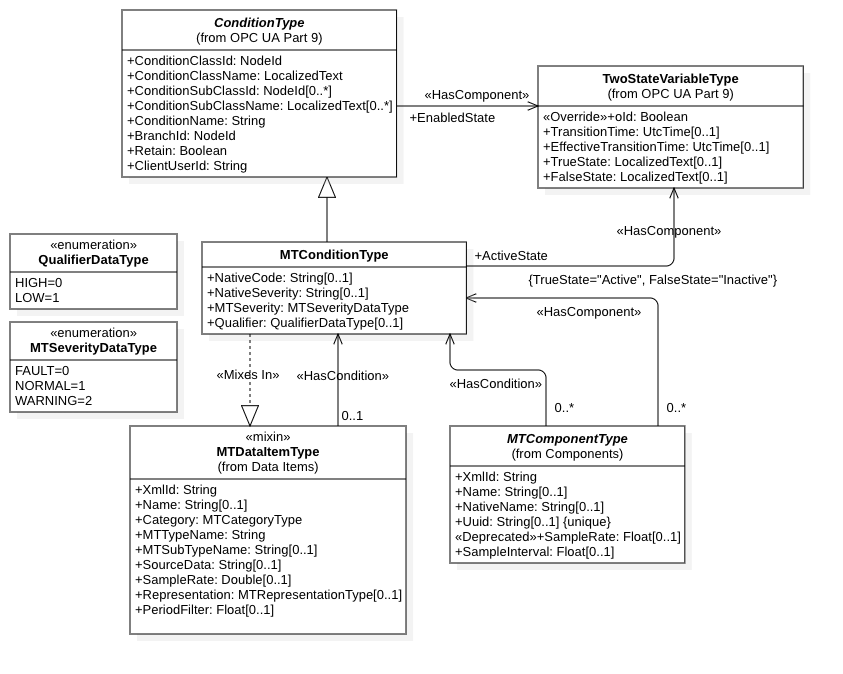
\includegraphics[width=1.0\textwidth]{./diagrams/types/Conditions.png}
  \caption{Conditions Diagram}
  \label{fig:Conditions}
\end{figure}

\FloatBarrier


\input ./type-sections/Conditions.tex

\subsubsection{Defintion of \texttt{ MTConditionType}}
  \label{type:MTConditionType}

\FloatBarrier

The condition type is a derived from the UA \mtmodel{ContitionType}. The Normal state of 
the condition is indicated by the ActiveState if \mtmodel{FALSE}. The severity 
is used to represent the MTConnect condition states of Warning and Fault with the values of
500 and 1000 respectively. 

An \mtmodel{MTConditionType} instance will be created for event MTConnect \gls{MTDataItem} with a 
\gls{category} of \mtmodel{CONDITION}. The \mtmodel{MTConditionType} instance will be instantiated 
with the \uamodel{Retain} flag set to true when the condition \uamodel{ActiveState} is true. 

The \gls{BrowseName} of the condition uses the same naming convention as the  MTConnect
\gls{MTDataItem} types with \gls{MTCondition} appended as a suffix. For example the 
condition with \gls{type} of \mtmodel{TEMPERATURE} will have the browse name of 
\mtmodel{TemperatureCondition} as opposed to the \mtuatype{MTSampleType} of \mtmodel{Temperature}.

If a \mtmodel{Source} of the \gls{MTDataItem} is provided, then the \uamodel{HasCondition} relationship 
will be from the source \gls{MTDataItem} to the \gls{MTCondition} instance. Otherwise it will be 
related to the MTConnect \gls{MTComponent} containing the \mtuatype{MTComponentType} instance.


\begin{table}[ht]
\centering 
  \caption{\texttt{MTConditionType} Definition}
  \label{table:MTConditionType}
\fontsize{9pt}{11pt}\selectfont
\tabulinesep=3pt
\begin{tabu} to 6in {|X[-1.35]|X[-0.7]|X[-1.75]|X[-1.5]|X[-1]|X[-0.7]|} \everyrow{\hline}
\hline
\rowfont\bfseries {Attribute} & \multicolumn{5}{|l|}{Value} \\
\tabucline[1.5pt]{}
BrowseName & \multicolumn{5}{|l|}{MTConditionType} \\
IsAbstract & \multicolumn{5}{|l|}{False} \\
\tabucline[1.5pt]{}
\rowfont \bfseries References & NodeClass & BrowseName & DataType & Type\-Definition & {Modeling\-Rule} \\
\multicolumn{6}{|l|}{Subtype of ConditionType (See \cite{UAPart9} Documentation)} \\
Has\-Property & Variable & Xml\-Id & String & Property\-Type & Mandatory \\
Has\-Property & Variable & Name & String & Property\-Type & Optional \\
Has\-Property & Variable & Category & MT\-Category\-Type & Property\-Type & Mandatory \\
Has\-Property & Variable & MT\-Type\-Name & String & Property\-Type & Mandatory \\
Has\-Property & Variable & MT\-Sub\-Type\-Name & String & Property\-Type & Optional \\
Has\-Property & Variable & Source\-Data & String & Property\-Type & Optional \\
Has\-Property & Variable & Sample\-Rate & Double & Property\-Type & Optional \\
Has\-Property & Variable & Representation & MT\-Representation\-Type & Property\-Type & Optional \\
Has\-Property & Variable & Period\-Filter & Float & Property\-Type & Optional \\
Has\-MT\-Class\-Type & Object & <MT\-Data\-Item\-Class> & \multicolumn{2}{l|}{MTDataItemClassType} & Mandatory \\
Has\-MT\-Sub\-Class\-Type & Object & <MT\-Data\-Item\-Sub\-Class> & \multicolumn{2}{l|}{MTDataItemSubClassType} & Optional \\
Has\-MT\-Composition & Object & <MT\-Composition> & \multicolumn{2}{l|}{MTCompositionType} & Optional \\
Has\-MT\-Source & Object & <Base\-Object> & \multicolumn{2}{l|}{BaseObjectType} & Optional \\
Has\-Condition & Event & <MT\-Condition> & \multicolumn{2}{l|}{MTConditionType} & Optional \\
Has\-Component & Object & Constraints & \multicolumn{2}{l|}{MTConstraintType} & Optional \\
Has\-Property & Variable & Native\-Code & String & Property\-Type & Optional \\
Has\-Property & Variable & Native\-Severity & String & Property\-Type & Optional \\
Has\-Property & Variable & MT\-Severity & MT\-Severity\-Data\-Type & Property\-Type & Mandatory \\
Has\-Property & Variable & Qualifier & Qualifier\-Data\-Type & Property\-Type & Optional \\
Has\-Component & Variable & Active\-State & Localized\-Text & Two\-State\-Variable\-Type & Mandatory \\
\end{tabu}
\end{table} 


\FloatBarrier
\paragraph{Referenced Properties and Objects}

\begin{itemize}
\item \texttt{NativeCode::String:} When instantiated in the address space this will represent the \mtmodel{NativeCode} of the last
\uaterm{Event} that was received. When the ActiveState becomes False and becomes 
inactive, then the \mtmodel{NativeCode} will be cleared.

\item \texttt{NativeSeverity::String:} When instantiated in the address space this will represent the \mtmodel{NativeSeverity} of the last
\uaterm{Event} that was received. When the ActiveState becomes False and becomes 
inactive, then the \mtmodel{NativeSeverity} will be cleared.

\item \textbf{Allowable Values} for \texttt{MTSeverityDataType}
\FloatBarrier
\begin{table}[ht]
\centering 
  \caption{\texttt{MTSeverityDataType} Enumeration}
  \label{enum:MTSeverityDataType}
\tabulinesep=3pt
\begin{tabu} to 6in {|l|r|} \everyrow{\hline}
\hline
\rowfont\bfseries {Name} & {Index} \\
\tabucline[1.5pt]{}
\texttt{FAULT} & \texttt{0} \\
\texttt{NORMAL} & \texttt{1} \\
\texttt{WARNING} & \texttt{2} \\
\end{tabu}
\end{table} 
\FloatBarrier
\item \textbf{Allowable Values} for \texttt{QualifierDataType}
\FloatBarrier
\begin{table}[ht]
\centering 
  \caption{\texttt{QualifierDataType} Enumeration}
  \label{enum:QualifierDataType}
\tabulinesep=3pt
\begin{tabu} to 6in {|l|r|} \everyrow{\hline}
\hline
\rowfont\bfseries {Name} & {Index} \\
\tabucline[1.5pt]{}
\texttt{HIGH} & \texttt{0} \\
\texttt{LOW} & \texttt{1} \\
\end{tabu}
\end{table} 
\FloatBarrier
\end{itemize}
\paragraph{Dependencies and Relationships}

\begin{itemize}
\item Mixes in \texttt{MTDataItemType}, see See section \ref{type:MTDataItemType}
\end{itemize}
\FloatBarrier
\subsection{Data Item Types} \label{model:DataItemTypes}

The data item types represent the MTConnect types as defined in Section 8 of the 
MTConnect Standard Part 2 \cite{MTCPart2} and are represented using the XML \gls{type} 
\mtmodel{attribute}. The type and sub-type relationships are given in the standard and are 
not documented in the companion specifiction. 

The model of the types is similar to the OPC UA condition classes as given in OPC UA Part 9
\cite{UAPart9}. Since MTConnect conditions use the same type system as the data items, 
the representation of the data item type will be derived from the \texttt{BaseConditionClassType}. 
The MTConnect Types will not use the \mtmodel{...ClassType}, but will be the name as specified
in the MTConnect standard with \mtmodel{Type} appended.

For example: The \mtmodel{CONTOLLER_MODE} will be given as the \mtmodel{ControllerModeType}. 
The relationship to the \gls{MTDataItem} OPC UA types are presented so that it will be
easier to map the MTConnect types to the correct super class as given in the OPC UA model.

\subsubsection{Defintion of \texttt{ MTDataItemClassType}}
  \label{type:MTDataItemClassType}

\FloatBarrier

Abstract base class for all the data item class types. The names are created by pascal typing the names
and then generating appending \mtmodel{Type}.

\begin{table}[ht]
\centering 
  \caption{\texttt{MTDataItemClassType} Definition}
  \label{table:MTDataItemClassType}
\fontsize{9pt}{11pt}\selectfont
\tabulinesep=3pt
\begin{tabu} to 6in {|X[-1.35]|X[-0.7]|X[-1.75]|X[-1.5]|X[-1]|X[-0.7]|} \everyrow{\hline}
\hline
\rowfont\bfseries {Attribute} & \multicolumn{5}{|l|}{Value} \\
\tabucline[1.5pt]{}
BrowseName & \multicolumn{5}{|l|}{MTDataItemClassType} \\
IsAbstract & \multicolumn{5}{|l|}{True} \\
\tabucline[1.5pt]{}
\rowfont \bfseries References & NodeClass & BrowseName & DataType & Type\-Definition & {Modeling\-Rule} \\
\multicolumn{6}{|l|}{Subtype of BaseConditionClassType (See \cite{UAPart9} Documentation)} \\
HasSubtype & ObjectType & \multicolumn{2}{l}{MTSampleClassType} & \multicolumn{2}{|l|}{See section \ref{type:MTSampleClassType}} \\
HasSubtype & ObjectType & \multicolumn{2}{l}{MTConditionClassType} & \multicolumn{2}{|l|}{See section \ref{type:MTConditionClassType}} \\
HasSubtype & ObjectType & \multicolumn{2}{l}{MTEventClassType} & \multicolumn{2}{|l|}{See section \ref{type:MTEventClassType}} \\
\end{tabu}
\end{table} 


\FloatBarrier
\subsubsection{Defintion of \texttt{ MTMessageClassType}}
  \label{type:MTMessageClassType}

\FloatBarrier
\begin{table}[ht]
\centering 
  \caption{\texttt{MTMessageClassType} Definition}
  \label{table:MTMessageClassType}
\fontsize{9pt}{11pt}\selectfont
\tabulinesep=3pt
\begin{tabu} to 6in {|X[-1.35]|X[-0.7]|X[-1.75]|X[-1.5]|X[-1]|X[-0.7]|} \everyrow{\hline}
\hline
\rowfont\bfseries {Attribute} & \multicolumn{5}{|l|}{Value} \\
\tabucline[1.5pt]{}
BrowseName & \multicolumn{5}{|l|}{MTMessageClassType} \\
IsAbstract & \multicolumn{5}{|l|}{False} \\
\tabucline[1.5pt]{}
\rowfont \bfseries References & NodeClass & BrowseName & DataType & Type\-Definition & {Modeling\-Rule} \\
\multicolumn{6}{|l|}{Subtype of MTEventClassType (See Data Items Documentation)} \\
\end{tabu}
\end{table} 


\FloatBarrier
\subsection{Sample Data Item Types} \label{model:SampleDataItemTypes}

The MTConnect Standard has the definitions of \glspl{Sample} in 
Section 8.1 of the MTConnect Standard Part 2 \cite{MTCPart2} and the definition of the 
values can be found in Section 5.3 of MTConnect Standard Part 3 \cite{MTCPart3}. 

The description of each type was copied from the MTConnect Standard,
but this not the definitive text for each type. For authoritative normative text, 
please refer to the sources \cite{MTCPart2} and \cite{MTCPart3}.

\subsubsection{Defintion of \texttt{ MTSampleClassType}}
  \label{type:MTSampleClassType}

\FloatBarrier

The base type class for all data items with a \gls{category} of \mtmodel{SAMPLE}.

\begin{table}[ht]
\centering 
  \caption{\texttt{MTSampleClassType} Definition}
  \label{table:MTSampleClassType}
\fontsize{9pt}{11pt}\selectfont
\tabulinesep=3pt
\begin{tabu} to 6in {|X[-1.35]|X[-0.7]|X[-1.75]|X[-1.5]|X[-1]|X[-0.7]|} \everyrow{\hline}
\hline
\rowfont\bfseries {Attribute} & \multicolumn{5}{|l|}{Value} \\
\tabucline[1.5pt]{}
BrowseName & \multicolumn{5}{|l|}{MTSampleClassType} \\
IsAbstract & \multicolumn{5}{|l|}{True} \\
\tabucline[1.5pt]{}
\rowfont \bfseries References & NodeClass & BrowseName & DataType & Type\-Definition & {Modeling\-Rule} \\
\multicolumn{6}{|l|}{Subtype of MTDataItemClassType (See Data Item Types Documentation)} \\
HasSubtype & ObjectType & \multicolumn{2}{l}{MassClassType} & \multicolumn{2}{|l|}{See section \ref{type:MassClassType}} \\
HasSubtype & ObjectType & \multicolumn{2}{l}{PathFeedrateClassType} & \multicolumn{2}{|l|}{See section \ref{type:PathFeedrateClassType}} \\
HasSubtype & ObjectType & \multicolumn{2}{l}{PathPositionClassType} & \multicolumn{2}{|l|}{See section \ref{type:PathPositionClassType}} \\
HasSubtype & ObjectType & \multicolumn{2}{l}{PHClassType} & \multicolumn{2}{|l|}{See section \ref{type:PHClassType}} \\
HasSubtype & ObjectType & \multicolumn{2}{l}{PositionClassType} & \multicolumn{2}{|l|}{See section \ref{type:PositionClassType}} \\
HasSubtype & ObjectType & \multicolumn{2}{l}{PowerFactorClassType} & \multicolumn{2}{|l|}{See section \ref{type:PowerFactorClassType}} \\
HasSubtype & ObjectType & \multicolumn{2}{l}{PressureClassType} & \multicolumn{2}{|l|}{See section \ref{type:PressureClassType}} \\
HasSubtype & ObjectType & \multicolumn{2}{l}{ProcessTimerClassType} & \multicolumn{2}{|l|}{See section \ref{type:ProcessTimerClassType}} \\
HasSubtype & ObjectType & \multicolumn{2}{l}{ResistenceClassType} & \multicolumn{2}{|l|}{See section \ref{type:ResistenceClassType}} \\
HasSubtype & ObjectType & \multicolumn{2}{l}{RotaryVelocityClassType} & \multicolumn{2}{|l|}{See section \ref{type:RotaryVelocityClassType}} \\
HasSubtype & ObjectType & \multicolumn{2}{l}{SoundLevelClassType} & \multicolumn{2}{|l|}{See section \ref{type:SoundLevelClassType}} \\
HasSubtype & ObjectType & \multicolumn{2}{l}{StrainClassType} & \multicolumn{2}{|l|}{See section \ref{type:StrainClassType}} \\
HasSubtype & ObjectType & \multicolumn{2}{l}{TemperatureClassType} & \multicolumn{2}{|l|}{See section \ref{type:TemperatureClassType}} \\
HasSubtype & ObjectType & \multicolumn{2}{l}{TensionClassType} & \multicolumn{2}{|l|}{See section \ref{type:TensionClassType}} \\
HasSubtype & ObjectType & \multicolumn{2}{l}{TiltClassType} & \multicolumn{2}{|l|}{See section \ref{type:TiltClassType}} \\
HasSubtype & ObjectType & \multicolumn{2}{l}{TorqueClassType} & \multicolumn{2}{|l|}{See section \ref{type:TorqueClassType}} \\
HasSubtype & ObjectType & \multicolumn{2}{l}{VoltAmpereClassType} & \multicolumn{2}{|l|}{See section \ref{type:VoltAmpereClassType}} \\
HasSubtype & ObjectType & \multicolumn{2}{l}{VelocityClassType} & \multicolumn{2}{|l|}{See section \ref{type:VelocityClassType}} \\
HasSubtype & ObjectType & \multicolumn{2}{l}{VoltAmpereReactiveClassType} & \multicolumn{2}{|l|}{See section \ref{type:VoltAmpereReactiveClassType}} \\
HasSubtype & ObjectType & \multicolumn{2}{l}{ViscosityClassType} & \multicolumn{2}{|l|}{See section \ref{type:ViscosityClassType}} \\
HasSubtype & ObjectType & \multicolumn{2}{l}{VoltageClassType} & \multicolumn{2}{|l|}{See section \ref{type:VoltageClassType}} \\
HasSubtype & ObjectType & \multicolumn{2}{l}{WattageClassType} & \multicolumn{2}{|l|}{See section \ref{type:WattageClassType}} \\
\multicolumn{6}{|l|}{Continued...} \\
\end{tabu}
\end{table}
\begin{table}[ht]
\fontsize{9pt}{11pt}\selectfont
\tabulinesep=3pt
\begin{tabu} to 6in {|X[-1.35]|X[-0.7]|X[-1.75]|X[-1.5]|X[-1]|X[-0.7]|} \everyrow{\hline}
\hline
\rowfont \bfseries References & NodeClass & BrowseName & DataType & Type\-Definition & {Modeling\-Rule} \\
HasSubtype & ObjectType & \multicolumn{2}{l}{LoadClassType} & \multicolumn{2}{|l|}{See section \ref{type:LoadClassType}} \\
HasSubtype & ObjectType & \multicolumn{2}{l}{AccelerationClassType} & \multicolumn{2}{|l|}{See section \ref{type:AccelerationClassType}} \\
HasSubtype & ObjectType & \multicolumn{2}{l}{AccumulatedTimeClassType} & \multicolumn{2}{|l|}{See section \ref{type:AccumulatedTimeClassType}} \\
HasSubtype & ObjectType & \multicolumn{2}{l}{AngularAccelerationClassType} & \multicolumn{2}{|l|}{See section \ref{type:AngularAccelerationClassType}} \\
HasSubtype & ObjectType & \multicolumn{2}{l}{AngularVelocityClassType} & \multicolumn{2}{|l|}{See section \ref{type:AngularVelocityClassType}} \\
HasSubtype & ObjectType & \multicolumn{2}{l}{AmperageClassType} & \multicolumn{2}{|l|}{See section \ref{type:AmperageClassType}} \\
HasSubtype & ObjectType & \multicolumn{2}{l}{AngleClassType} & \multicolumn{2}{|l|}{See section \ref{type:AngleClassType}} \\
HasSubtype & ObjectType & \multicolumn{2}{l}{AxisFeedrateClassType} & \multicolumn{2}{|l|}{See section \ref{type:AxisFeedrateClassType}} \\
HasSubtype & ObjectType & \multicolumn{2}{l}{ClockTimeClassType} & \multicolumn{2}{|l|}{See section \ref{type:ClockTimeClassType}} \\
HasSubtype & ObjectType & \multicolumn{2}{l}{ConcentrationClassType} & \multicolumn{2}{|l|}{See section \ref{type:ConcentrationClassType}} \\
HasSubtype & ObjectType & \multicolumn{2}{l}{ConductivityClassType} & \multicolumn{2}{|l|}{See section \ref{type:ConductivityClassType}} \\
HasSubtype & ObjectType & \multicolumn{2}{l}{DisplacementClassType} & \multicolumn{2}{|l|}{See section \ref{type:DisplacementClassType}} \\
HasSubtype & ObjectType & \multicolumn{2}{l}{ElectricalEnergyClassType} & \multicolumn{2}{|l|}{See section \ref{type:ElectricalEnergyClassType}} \\
HasSubtype & ObjectType & \multicolumn{2}{l}{EquipmentTimerClassType} & \multicolumn{2}{|l|}{See section \ref{type:EquipmentTimerClassType}} \\
HasSubtype & ObjectType & \multicolumn{2}{l}{FillLevelClassType} & \multicolumn{2}{|l|}{See section \ref{type:FillLevelClassType}} \\
HasSubtype & ObjectType & \multicolumn{2}{l}{FlowClassType} & \multicolumn{2}{|l|}{See section \ref{type:FlowClassType}} \\
HasSubtype & ObjectType & \multicolumn{2}{l}{FrequencyClassType} & \multicolumn{2}{|l|}{See section \ref{type:FrequencyClassType}} \\
HasSubtype & ObjectType & \multicolumn{2}{l}{LengthClassType} & \multicolumn{2}{|l|}{See section \ref{type:LengthClassType}} \\
HasSubtype & ObjectType & \multicolumn{2}{l}{LinearForceClassType} & \multicolumn{2}{|l|}{See section \ref{type:LinearForceClassType}} \\
\end{tabu}
\end{table} 


\FloatBarrier
\subsubsection{Defintion of \texttt{ LoadClassType}}
  \label{type:LoadClassType}

\FloatBarrier

The measurement of the actual versus the standard rating of a piece of equipment. $PERCENT$

\begin{table}[ht]
\centering 
  \caption{\texttt{LoadClassType} Definition}
  \label{table:LoadClassType}
\fontsize{9pt}{11pt}\selectfont
\tabulinesep=3pt
\begin{tabu} to 6in {|X[-1.35]|X[-0.7]|X[-1.75]|X[-1.5]|X[-1]|X[-0.7]|} \everyrow{\hline}
\hline
\rowfont\bfseries {Attribute} & \multicolumn{5}{|l|}{Value} \\
\tabucline[1.5pt]{}
BrowseName & \multicolumn{5}{|l|}{LoadClassType} \\
IsAbstract & \multicolumn{5}{|l|}{False} \\
\tabucline[1.5pt]{}
\rowfont \bfseries References & NodeClass & BrowseName & DataType & Type\-Definition & {Modeling\-Rule} \\
\multicolumn{6}{|l|}{Subtype of MTSampleClassType (See section \ref{type:MTSampleClassType})} \\
\end{tabu}
\end{table} 


\FloatBarrier
\subsubsection{Defintion of \texttt{ AccelerationClassType}}
  \label{type:AccelerationClassType}

\FloatBarrier

Rate of change of velocity. $\frac{MILLIMETER}{SECOND^{2}}$

\begin{table}[ht]
\centering 
  \caption{\texttt{AccelerationClassType} Definition}
  \label{table:AccelerationClassType}
\fontsize{9pt}{11pt}\selectfont
\tabulinesep=3pt
\begin{tabu} to 6in {|X[-1.35]|X[-0.7]|X[-1.75]|X[-1.5]|X[-1]|X[-0.7]|} \everyrow{\hline}
\hline
\rowfont\bfseries {Attribute} & \multicolumn{5}{|l|}{Value} \\
\tabucline[1.5pt]{}
BrowseName & \multicolumn{5}{|l|}{AccelerationClassType} \\
IsAbstract & \multicolumn{5}{|l|}{False} \\
\tabucline[1.5pt]{}
\rowfont \bfseries References & NodeClass & BrowseName & DataType & Type\-Definition & {Modeling\-Rule} \\
\multicolumn{6}{|l|}{Subtype of MTSampleClassType (See section \ref{type:MTSampleClassType})} \\
\end{tabu}
\end{table} 


\FloatBarrier
\subsubsection{Defintion of \texttt{ AccumulatedTimeClassType}}
  \label{type:AccumulatedTimeClassType}

\FloatBarrier

The measurement of accumulated time for an activity or event. $SECOND$


\begin{table}[ht]
\centering 
  \caption{\texttt{AccumulatedTimeClassType} Definition}
  \label{table:AccumulatedTimeClassType}
\fontsize{9pt}{11pt}\selectfont
\tabulinesep=3pt
\begin{tabu} to 6in {|X[-1.35]|X[-0.7]|X[-1.75]|X[-1.5]|X[-1]|X[-0.7]|} \everyrow{\hline}
\hline
\rowfont\bfseries {Attribute} & \multicolumn{5}{|l|}{Value} \\
\tabucline[1.5pt]{}
BrowseName & \multicolumn{5}{|l|}{AccumulatedTimeClassType} \\
IsAbstract & \multicolumn{5}{|l|}{False} \\
\tabucline[1.5pt]{}
\rowfont \bfseries References & NodeClass & BrowseName & DataType & Type\-Definition & {Modeling\-Rule} \\
\multicolumn{6}{|l|}{Subtype of MTSampleClassType (See section \ref{type:MTSampleClassType})} \\
\end{tabu}
\end{table} 


\FloatBarrier
\subsubsection{Defintion of \texttt{ AngularAccelerationClassType}}
  \label{type:AngularAccelerationClassType}

\FloatBarrier

Rate of change of angular velocity.  $\frac{DEGREE}{SECOND^{2}}$

\begin{table}[ht]
\centering 
  \caption{\texttt{AngularAccelerationClassType} Definition}
  \label{table:AngularAccelerationClassType}
\fontsize{9pt}{11pt}\selectfont
\tabulinesep=3pt
\begin{tabu} to 6in {|X[-1.35]|X[-0.7]|X[-1.75]|X[-1.5]|X[-1]|X[-0.7]|} \everyrow{\hline}
\hline
\rowfont\bfseries {Attribute} & \multicolumn{5}{|l|}{Value} \\
\tabucline[1.5pt]{}
BrowseName & \multicolumn{5}{|l|}{AngularAccelerationClassType} \\
IsAbstract & \multicolumn{5}{|l|}{False} \\
\tabucline[1.5pt]{}
\rowfont \bfseries References & NodeClass & BrowseName & DataType & Type\-Definition & {Modeling\-Rule} \\
\multicolumn{6}{|l|}{Subtype of MTSampleClassType (See section \ref{type:MTSampleClassType})} \\
\end{tabu}
\end{table} 


\FloatBarrier
\subsubsection{Defintion of \texttt{ AngularVelocityClassType}}
  \label{type:AngularVelocityClassType}

\FloatBarrier

Rate of change of angular position. $\frac{DEGREE}{SECOND}$

\begin{table}[ht]
\centering 
  \caption{\texttt{AngularVelocityClassType} Definition}
  \label{table:AngularVelocityClassType}
\fontsize{9pt}{11pt}\selectfont
\tabulinesep=3pt
\begin{tabu} to 6in {|X[-1.35]|X[-0.7]|X[-1.75]|X[-1.5]|X[-1]|X[-0.7]|} \everyrow{\hline}
\hline
\rowfont\bfseries {Attribute} & \multicolumn{5}{|l|}{Value} \\
\tabucline[1.5pt]{}
BrowseName & \multicolumn{5}{|l|}{AngularVelocityClassType} \\
IsAbstract & \multicolumn{5}{|l|}{False} \\
\tabucline[1.5pt]{}
\rowfont \bfseries References & NodeClass & BrowseName & DataType & Type\-Definition & {Modeling\-Rule} \\
\multicolumn{6}{|l|}{Subtype of MTSampleClassType (See section \ref{type:MTSampleClassType})} \\
\end{tabu}
\end{table} 


\FloatBarrier
\subsubsection{Defintion of \texttt{ AmperageClassType}}
  \label{type:AmperageClassType}

\FloatBarrier

The measurement of electrical current. $AMPERE$

\begin{table}[ht]
\centering 
  \caption{\texttt{AmperageClassType} Definition}
  \label{table:AmperageClassType}
\fontsize{9pt}{11pt}\selectfont
\tabulinesep=3pt
\begin{tabu} to 6in {|X[-1.35]|X[-0.7]|X[-1.75]|X[-1.5]|X[-1]|X[-0.7]|} \everyrow{\hline}
\hline
\rowfont\bfseries {Attribute} & \multicolumn{5}{|l|}{Value} \\
\tabucline[1.5pt]{}
BrowseName & \multicolumn{5}{|l|}{AmperageClassType} \\
IsAbstract & \multicolumn{5}{|l|}{False} \\
\tabucline[1.5pt]{}
\rowfont \bfseries References & NodeClass & BrowseName & DataType & Type\-Definition & {Modeling\-Rule} \\
\multicolumn{6}{|l|}{Subtype of MTSampleClassType (See section \ref{type:MTSampleClassType})} \\
\end{tabu}
\end{table} 


\FloatBarrier
\subsubsection{Defintion of \texttt{ AngleClassType}}
  \label{type:AngleClassType}

\FloatBarrier

The measurement of angular position. $DEGREE$

\begin{table}[ht]
\centering 
  \caption{\texttt{AngleClassType} Definition}
  \label{table:AngleClassType}
\fontsize{9pt}{11pt}\selectfont
\tabulinesep=3pt
\begin{tabu} to 6in {|X[-1.35]|X[-0.7]|X[-1.75]|X[-1.5]|X[-1]|X[-0.7]|} \everyrow{\hline}
\hline
\rowfont\bfseries {Attribute} & \multicolumn{5}{|l|}{Value} \\
\tabucline[1.5pt]{}
BrowseName & \multicolumn{5}{|l|}{AngleClassType} \\
IsAbstract & \multicolumn{5}{|l|}{False} \\
\tabucline[1.5pt]{}
\rowfont \bfseries References & NodeClass & BrowseName & DataType & Type\-Definition & {Modeling\-Rule} \\
\multicolumn{6}{|l|}{Subtype of MTSampleClassType (See section \ref{type:MTSampleClassType})} \\
\end{tabu}
\end{table} 


\FloatBarrier
\subsubsection{Defintion of \texttt{ AxisFeedrateClassType}}
  \label{type:AxisFeedrateClassType}

\FloatBarrier

The feedrate of a linear axis. $\frac{MILLIMETER}{SECOND}$

\begin{table}[ht]
\centering 
  \caption{\texttt{AxisFeedrateClassType} Definition}
  \label{table:AxisFeedrateClassType}
\fontsize{9pt}{11pt}\selectfont
\tabulinesep=3pt
\begin{tabu} to 6in {|X[-1.35]|X[-0.7]|X[-1.75]|X[-1.5]|X[-1]|X[-0.7]|} \everyrow{\hline}
\hline
\rowfont\bfseries {Attribute} & \multicolumn{5}{|l|}{Value} \\
\tabucline[1.5pt]{}
BrowseName & \multicolumn{5}{|l|}{AxisFeedrateClassType} \\
IsAbstract & \multicolumn{5}{|l|}{False} \\
\tabucline[1.5pt]{}
\rowfont \bfseries References & NodeClass & BrowseName & DataType & Type\-Definition & {Modeling\-Rule} \\
\multicolumn{6}{|l|}{Subtype of MTSampleClassType (See section \ref{type:MTSampleClassType})} \\
\end{tabu}
\end{table} 


\FloatBarrier
\subsubsection{Defintion of \texttt{ ClockTimeClassType}}
  \label{type:ClockTimeClassType}

\FloatBarrier

The value provided by a timing device at a specific point in time. $TIMESTAMP$

\begin{table}[ht]
\centering 
  \caption{\texttt{ClockTimeClassType} Definition}
  \label{table:ClockTimeClassType}
\fontsize{9pt}{11pt}\selectfont
\tabulinesep=3pt
\begin{tabu} to 6in {|X[-1.35]|X[-0.7]|X[-1.75]|X[-1.5]|X[-1]|X[-0.7]|} \everyrow{\hline}
\hline
\rowfont\bfseries {Attribute} & \multicolumn{5}{|l|}{Value} \\
\tabucline[1.5pt]{}
BrowseName & \multicolumn{5}{|l|}{ClockTimeClassType} \\
IsAbstract & \multicolumn{5}{|l|}{False} \\
\tabucline[1.5pt]{}
\rowfont \bfseries References & NodeClass & BrowseName & DataType & Type\-Definition & {Modeling\-Rule} \\
\multicolumn{6}{|l|}{Subtype of MTSampleClassType (See section \ref{type:MTSampleClassType})} \\
\end{tabu}
\end{table} 


\FloatBarrier
\subsubsection{Defintion of \texttt{ ConcentrationClassType}}
  \label{type:ConcentrationClassType}

\FloatBarrier

Percentage of one component within a mixture of components. $PERCENT$

\begin{table}[ht]
\centering 
  \caption{\texttt{ConcentrationClassType} Definition}
  \label{table:ConcentrationClassType}
\fontsize{9pt}{11pt}\selectfont
\tabulinesep=3pt
\begin{tabu} to 6in {|X[-1.35]|X[-0.7]|X[-1.75]|X[-1.5]|X[-1]|X[-0.7]|} \everyrow{\hline}
\hline
\rowfont\bfseries {Attribute} & \multicolumn{5}{|l|}{Value} \\
\tabucline[1.5pt]{}
BrowseName & \multicolumn{5}{|l|}{ConcentrationClassType} \\
IsAbstract & \multicolumn{5}{|l|}{False} \\
\tabucline[1.5pt]{}
\rowfont \bfseries References & NodeClass & BrowseName & DataType & Type\-Definition & {Modeling\-Rule} \\
\multicolumn{6}{|l|}{Subtype of MTSampleClassType (See section \ref{type:MTSampleClassType})} \\
\end{tabu}
\end{table} 


\FloatBarrier
\subsubsection{Defintion of \texttt{ ConductivityClassType}}
  \label{type:ConductivityClassType}

\FloatBarrier

The ability of a material to conduct electricity. $\frac{SIEMENS}{METER}$

\begin{table}[ht]
\centering 
  \caption{\texttt{ConductivityClassType} Definition}
  \label{table:ConductivityClassType}
\fontsize{9pt}{11pt}\selectfont
\tabulinesep=3pt
\begin{tabu} to 6in {|X[-1.35]|X[-0.7]|X[-1.75]|X[-1.5]|X[-1]|X[-0.7]|} \everyrow{\hline}
\hline
\rowfont\bfseries {Attribute} & \multicolumn{5}{|l|}{Value} \\
\tabucline[1.5pt]{}
BrowseName & \multicolumn{5}{|l|}{ConductivityClassType} \\
IsAbstract & \multicolumn{5}{|l|}{False} \\
\tabucline[1.5pt]{}
\rowfont \bfseries References & NodeClass & BrowseName & DataType & Type\-Definition & {Modeling\-Rule} \\
\multicolumn{6}{|l|}{Subtype of MTSampleClassType (See section \ref{type:MTSampleClassType})} \\
\end{tabu}
\end{table} 


\FloatBarrier
\subsubsection{Defintion of \texttt{ DisplacementClassType}}
  \label{type:DisplacementClassType}

\FloatBarrier

The change in position of an object. $MILLIMETER$

\begin{table}[ht]
\centering 
  \caption{\texttt{DisplacementClassType} Definition}
  \label{table:DisplacementClassType}
\fontsize{9pt}{11pt}\selectfont
\tabulinesep=3pt
\begin{tabu} to 6in {|X[-1.35]|X[-0.7]|X[-1.75]|X[-1.5]|X[-1]|X[-0.7]|} \everyrow{\hline}
\hline
\rowfont\bfseries {Attribute} & \multicolumn{5}{|l|}{Value} \\
\tabucline[1.5pt]{}
BrowseName & \multicolumn{5}{|l|}{DisplacementClassType} \\
IsAbstract & \multicolumn{5}{|l|}{False} \\
\tabucline[1.5pt]{}
\rowfont \bfseries References & NodeClass & BrowseName & DataType & Type\-Definition & {Modeling\-Rule} \\
\multicolumn{6}{|l|}{Subtype of MTSampleClassType (See section \ref{type:MTSampleClassType})} \\
\end{tabu}
\end{table} 


\FloatBarrier
\subsubsection{Defintion of \texttt{ ElectricalEnergyClassType}}
  \label{type:ElectricalEnergyClassType}

\FloatBarrier

The measurement of electrical energy consumption by a component. $WATT \times SECOND$

\begin{table}[ht]
\centering 
  \caption{\texttt{ElectricalEnergyClassType} Definition}
  \label{table:ElectricalEnergyClassType}
\fontsize{9pt}{11pt}\selectfont
\tabulinesep=3pt
\begin{tabu} to 6in {|X[-1.35]|X[-0.7]|X[-1.75]|X[-1.5]|X[-1]|X[-0.7]|} \everyrow{\hline}
\hline
\rowfont\bfseries {Attribute} & \multicolumn{5}{|l|}{Value} \\
\tabucline[1.5pt]{}
BrowseName & \multicolumn{5}{|l|}{ElectricalEnergyClassType} \\
IsAbstract & \multicolumn{5}{|l|}{False} \\
\tabucline[1.5pt]{}
\rowfont \bfseries References & NodeClass & BrowseName & DataType & Type\-Definition & {Modeling\-Rule} \\
\multicolumn{6}{|l|}{Subtype of MTSampleClassType (See section \ref{type:MTSampleClassType})} \\
\end{tabu}
\end{table} 


\FloatBarrier
\subsubsection{Defintion of \texttt{ EquipmentTimerClassType}}
  \label{type:EquipmentTimerClassType}

\FloatBarrier

The measurement of the amount of time a \mtmodel{SECOND} piece of equipment or a sub-part of a 
piece of equipment has performed specific activities. 
Often used to determine when maintenance may be required for the equipment.
 
 
Multiple subTypes of \mtmodel{EQUIPMENT_TIMER} MAY be defined.
A subType MUST always be specified.

$SECOND$

\begin{table}[ht]
\centering 
  \caption{\texttt{EquipmentTimerClassType} Definition}
  \label{table:EquipmentTimerClassType}
\fontsize{9pt}{11pt}\selectfont
\tabulinesep=3pt
\begin{tabu} to 6in {|X[-1.35]|X[-0.7]|X[-1.75]|X[-1.5]|X[-1]|X[-0.7]|} \everyrow{\hline}
\hline
\rowfont\bfseries {Attribute} & \multicolumn{5}{|l|}{Value} \\
\tabucline[1.5pt]{}
BrowseName & \multicolumn{5}{|l|}{EquipmentTimerClassType} \\
IsAbstract & \multicolumn{5}{|l|}{False} \\
\tabucline[1.5pt]{}
\rowfont \bfseries References & NodeClass & BrowseName & DataType & Type\-Definition & {Modeling\-Rule} \\
\multicolumn{6}{|l|}{Subtype of MTSampleClassType (See section \ref{type:MTSampleClassType})} \\
\end{tabu}
\end{table} 


\FloatBarrier
\subsubsection{Defintion of \texttt{ FillLevelClassType}}
  \label{type:FillLevelClassType}

\FloatBarrier

The measurement of the amount of a substance remaining compared to the planned 
maximum amount of that substance. $PERCENT$

\begin{table}[ht]
\centering 
  \caption{\texttt{FillLevelClassType} Definition}
  \label{table:FillLevelClassType}
\fontsize{9pt}{11pt}\selectfont
\tabulinesep=3pt
\begin{tabu} to 6in {|X[-1.35]|X[-0.7]|X[-1.75]|X[-1.5]|X[-1]|X[-0.7]|} \everyrow{\hline}
\hline
\rowfont\bfseries {Attribute} & \multicolumn{5}{|l|}{Value} \\
\tabucline[1.5pt]{}
BrowseName & \multicolumn{5}{|l|}{FillLevelClassType} \\
IsAbstract & \multicolumn{5}{|l|}{False} \\
\tabucline[1.5pt]{}
\rowfont \bfseries References & NodeClass & BrowseName & DataType & Type\-Definition & {Modeling\-Rule} \\
\multicolumn{6}{|l|}{Subtype of MTSampleClassType (See section \ref{type:MTSampleClassType})} \\
\end{tabu}
\end{table} 


\FloatBarrier
\subsubsection{Defintion of \texttt{ FlowClassType}}
  \label{type:FlowClassType}

\FloatBarrier

The rate of flow of a fluid. $\frac{LITER}{SECOND}$

\begin{table}[ht]
\centering 
  \caption{\texttt{FlowClassType} Definition}
  \label{table:FlowClassType}
\fontsize{9pt}{11pt}\selectfont
\tabulinesep=3pt
\begin{tabu} to 6in {|X[-1.35]|X[-0.7]|X[-1.75]|X[-1.5]|X[-1]|X[-0.7]|} \everyrow{\hline}
\hline
\rowfont\bfseries {Attribute} & \multicolumn{5}{|l|}{Value} \\
\tabucline[1.5pt]{}
BrowseName & \multicolumn{5}{|l|}{FlowClassType} \\
IsAbstract & \multicolumn{5}{|l|}{False} \\
\tabucline[1.5pt]{}
\rowfont \bfseries References & NodeClass & BrowseName & DataType & Type\-Definition & {Modeling\-Rule} \\
\multicolumn{6}{|l|}{Subtype of MTSampleClassType (See section \ref{type:MTSampleClassType})} \\
\end{tabu}
\end{table} 


\FloatBarrier
\subsubsection{Defintion of \texttt{ FrequencyClassType}}
  \label{type:FrequencyClassType}

\FloatBarrier

The measurement of the number of occurrences of a repeating event per unit time. $HERTZ$


\begin{table}[ht]
\centering 
  \caption{\texttt{FrequencyClassType} Definition}
  \label{table:FrequencyClassType}
\fontsize{9pt}{11pt}\selectfont
\tabulinesep=3pt
\begin{tabu} to 6in {|X[-1.35]|X[-0.7]|X[-1.75]|X[-1.5]|X[-1]|X[-0.7]|} \everyrow{\hline}
\hline
\rowfont\bfseries {Attribute} & \multicolumn{5}{|l|}{Value} \\
\tabucline[1.5pt]{}
BrowseName & \multicolumn{5}{|l|}{FrequencyClassType} \\
IsAbstract & \multicolumn{5}{|l|}{False} \\
\tabucline[1.5pt]{}
\rowfont \bfseries References & NodeClass & BrowseName & DataType & Type\-Definition & {Modeling\-Rule} \\
\multicolumn{6}{|l|}{Subtype of MTSampleClassType (See section \ref{type:MTSampleClassType})} \\
\end{tabu}
\end{table} 


\FloatBarrier
\subsubsection{Defintion of \texttt{ LengthClassType}}
  \label{type:LengthClassType}

\FloatBarrier

The length of an object. $MILLIMETER$

\begin{table}[ht]
\centering 
  \caption{\texttt{LengthClassType} Definition}
  \label{table:LengthClassType}
\fontsize{9pt}{11pt}\selectfont
\tabulinesep=3pt
\begin{tabu} to 6in {|X[-1.35]|X[-0.7]|X[-1.75]|X[-1.5]|X[-1]|X[-0.7]|} \everyrow{\hline}
\hline
\rowfont\bfseries {Attribute} & \multicolumn{5}{|l|}{Value} \\
\tabucline[1.5pt]{}
BrowseName & \multicolumn{5}{|l|}{LengthClassType} \\
IsAbstract & \multicolumn{5}{|l|}{False} \\
\tabucline[1.5pt]{}
\rowfont \bfseries References & NodeClass & BrowseName & DataType & Type\-Definition & {Modeling\-Rule} \\
\multicolumn{6}{|l|}{Subtype of MTSampleClassType (See section \ref{type:MTSampleClassType})} \\
\end{tabu}
\end{table} 


\FloatBarrier
\paragraph{Referenced Properties and Objects}

\begin{itemize}
\item \texttt{Supertype::MTSampleClassType:} The length of an object

\end{itemize}
\FloatBarrier
\subsubsection{Defintion of \texttt{ LinearForceClassType}}
  \label{type:LinearForceClassType}

\FloatBarrier

The measure of the push or pull introduced by an actuator or exerted on an object. $NEWTON$

\begin{table}[ht]
\centering 
  \caption{\texttt{LinearForceClassType} Definition}
  \label{table:LinearForceClassType}
\fontsize{9pt}{11pt}\selectfont
\tabulinesep=3pt
\begin{tabu} to 6in {|X[-1.35]|X[-0.7]|X[-1.75]|X[-1.5]|X[-1]|X[-0.7]|} \everyrow{\hline}
\hline
\rowfont\bfseries {Attribute} & \multicolumn{5}{|l|}{Value} \\
\tabucline[1.5pt]{}
BrowseName & \multicolumn{5}{|l|}{LinearForceClassType} \\
IsAbstract & \multicolumn{5}{|l|}{False} \\
\tabucline[1.5pt]{}
\rowfont \bfseries References & NodeClass & BrowseName & DataType & Type\-Definition & {Modeling\-Rule} \\
\multicolumn{6}{|l|}{Subtype of MTSampleClassType (See section \ref{type:MTSampleClassType})} \\
\end{tabu}
\end{table} 


\FloatBarrier
\subsubsection{Defintion of \texttt{ MassClassType}}
  \label{type:MassClassType}

\FloatBarrier

The measurement of the mass of an object(s) or an amount of material. $KILOGRAM$

\begin{table}[ht]
\centering 
  \caption{\texttt{MassClassType} Definition}
  \label{table:MassClassType}
\fontsize{9pt}{11pt}\selectfont
\tabulinesep=3pt
\begin{tabu} to 6in {|X[-1.35]|X[-0.7]|X[-1.75]|X[-1.5]|X[-1]|X[-0.7]|} \everyrow{\hline}
\hline
\rowfont\bfseries {Attribute} & \multicolumn{5}{|l|}{Value} \\
\tabucline[1.5pt]{}
BrowseName & \multicolumn{5}{|l|}{MassClassType} \\
IsAbstract & \multicolumn{5}{|l|}{False} \\
\tabucline[1.5pt]{}
\rowfont \bfseries References & NodeClass & BrowseName & DataType & Type\-Definition & {Modeling\-Rule} \\
\multicolumn{6}{|l|}{Subtype of MTSampleClassType (See section \ref{type:MTSampleClassType})} \\
\end{tabu}
\end{table} 


\FloatBarrier
\subsubsection{Defintion of \texttt{ PathFeedrateClassType}}
  \label{type:PathFeedrateClassType}

\FloatBarrier

The feedrate for the axes, or a single axis, associated with a \mtmodel{Path} component 
a vector. $\frac{MILLIMETER}{SECOND}$

\begin{table}[ht]
\centering 
  \caption{\texttt{PathFeedrateClassType} Definition}
  \label{table:PathFeedrateClassType}
\fontsize{9pt}{11pt}\selectfont
\tabulinesep=3pt
\begin{tabu} to 6in {|X[-1.35]|X[-0.7]|X[-1.75]|X[-1.5]|X[-1]|X[-0.7]|} \everyrow{\hline}
\hline
\rowfont\bfseries {Attribute} & \multicolumn{5}{|l|}{Value} \\
\tabucline[1.5pt]{}
BrowseName & \multicolumn{5}{|l|}{PathFeedrateClassType} \\
IsAbstract & \multicolumn{5}{|l|}{False} \\
\tabucline[1.5pt]{}
\rowfont \bfseries References & NodeClass & BrowseName & DataType & Type\-Definition & {Modeling\-Rule} \\
\multicolumn{6}{|l|}{Subtype of MTSampleClassType (See section \ref{type:MTSampleClassType})} \\
\end{tabu}
\end{table} 


\FloatBarrier
\subsubsection{Defintion of \texttt{ PathPositionClassType}}
  \label{type:PathPositionClassType}

\FloatBarrier

A measured or calculated position of a control point associated with a \mtmodel{Controller} element, 
or PATH element if provided, of a piece of equipment.

The control point MUST be reported as a set of space-delimited floating-point 
numbers representing a point in 3-D space. The position of the control point MUST 
be reported in units of \mtmodel{MILLIMETER} and listed in order of X, Y, and Z 
referenced to the coordinate system of the piece of equipment.

$MILLIMETER (\mathbb{R}^{3})$

\begin{table}[ht]
\centering 
  \caption{\texttt{PathPositionClassType} Definition}
  \label{table:PathPositionClassType}
\fontsize{9pt}{11pt}\selectfont
\tabulinesep=3pt
\begin{tabu} to 6in {|X[-1.35]|X[-0.7]|X[-1.75]|X[-1.5]|X[-1]|X[-0.7]|} \everyrow{\hline}
\hline
\rowfont\bfseries {Attribute} & \multicolumn{5}{|l|}{Value} \\
\tabucline[1.5pt]{}
BrowseName & \multicolumn{5}{|l|}{PathPositionClassType} \\
IsAbstract & \multicolumn{5}{|l|}{False} \\
\tabucline[1.5pt]{}
\rowfont \bfseries References & NodeClass & BrowseName & DataType & Type\-Definition & {Modeling\-Rule} \\
\multicolumn{6}{|l|}{Subtype of MTSampleClassType (See section \ref{type:MTSampleClassType})} \\
\end{tabu}
\end{table} 


\FloatBarrier
\subsubsection{Defintion of \texttt{ PHClassType}}
  \label{type:PHClassType}

\FloatBarrier

The measure of the acidity or alkalinity. $PH$

\begin{table}[ht]
\centering 
  \caption{\texttt{PHClassType} Definition}
  \label{table:PHClassType}
\fontsize{9pt}{11pt}\selectfont
\tabulinesep=3pt
\begin{tabu} to 6in {|X[-1.35]|X[-0.7]|X[-1.75]|X[-1.5]|X[-1]|X[-0.7]|} \everyrow{\hline}
\hline
\rowfont\bfseries {Attribute} & \multicolumn{5}{|l|}{Value} \\
\tabucline[1.5pt]{}
BrowseName & \multicolumn{5}{|l|}{PHClassType} \\
IsAbstract & \multicolumn{5}{|l|}{False} \\
\tabucline[1.5pt]{}
\rowfont \bfseries References & NodeClass & BrowseName & DataType & Type\-Definition & {Modeling\-Rule} \\
\multicolumn{6}{|l|}{Subtype of MTSampleClassType (See section \ref{type:MTSampleClassType})} \\
\end{tabu}
\end{table} 


\FloatBarrier
\subsubsection{Defintion of \texttt{ PositionClassType}}
  \label{type:PositionClassType}

\FloatBarrier

A calculated or measured position related to a Component element.

\mtmodel{POSITION} SHOULD be further defined withacoordinateSytemattribute. 
If a coordinateSystem attribute is not specified, the position of the control point 
MUST be reported in \mtmodel{MACHINE} coordinates. 

$MILLIMETER$

\begin{table}[ht]
\centering 
  \caption{\texttt{PositionClassType} Definition}
  \label{table:PositionClassType}
\fontsize{9pt}{11pt}\selectfont
\tabulinesep=3pt
\begin{tabu} to 6in {|X[-1.35]|X[-0.7]|X[-1.75]|X[-1.5]|X[-1]|X[-0.7]|} \everyrow{\hline}
\hline
\rowfont\bfseries {Attribute} & \multicolumn{5}{|l|}{Value} \\
\tabucline[1.5pt]{}
BrowseName & \multicolumn{5}{|l|}{PositionClassType} \\
IsAbstract & \multicolumn{5}{|l|}{False} \\
\tabucline[1.5pt]{}
\rowfont \bfseries References & NodeClass & BrowseName & DataType & Type\-Definition & {Modeling\-Rule} \\
\multicolumn{6}{|l|}{Subtype of MTSampleClassType (See section \ref{type:MTSampleClassType})} \\
\end{tabu}
\end{table} 


\FloatBarrier
\subsubsection{Defintion of \texttt{ PowerFactorClassType}}
  \label{type:PowerFactorClassType}

\FloatBarrier

The measurement of the ratio of real power flowing to a load to the apparent power in
that AC circuit. $PERCENT$

\begin{table}[ht]
\centering 
  \caption{\texttt{PowerFactorClassType} Definition}
  \label{table:PowerFactorClassType}
\fontsize{9pt}{11pt}\selectfont
\tabulinesep=3pt
\begin{tabu} to 6in {|X[-1.35]|X[-0.7]|X[-1.75]|X[-1.5]|X[-1]|X[-0.7]|} \everyrow{\hline}
\hline
\rowfont\bfseries {Attribute} & \multicolumn{5}{|l|}{Value} \\
\tabucline[1.5pt]{}
BrowseName & \multicolumn{5}{|l|}{PowerFactorClassType} \\
IsAbstract & \multicolumn{5}{|l|}{False} \\
\tabucline[1.5pt]{}
\rowfont \bfseries References & NodeClass & BrowseName & DataType & Type\-Definition & {Modeling\-Rule} \\
\multicolumn{6}{|l|}{Subtype of MTSampleClassType (See section \ref{type:MTSampleClassType})} \\
\end{tabu}
\end{table} 


\FloatBarrier
\subsubsection{Defintion of \texttt{ PressureClassType}}
  \label{type:PressureClassType}

\FloatBarrier

The force per unit area exerted by a gas or liquid. $PASCAL$

\begin{table}[ht]
\centering 
  \caption{\texttt{PressureClassType} Definition}
  \label{table:PressureClassType}
\fontsize{9pt}{11pt}\selectfont
\tabulinesep=3pt
\begin{tabu} to 6in {|X[-1.35]|X[-0.7]|X[-1.75]|X[-1.5]|X[-1]|X[-0.7]|} \everyrow{\hline}
\hline
\rowfont\bfseries {Attribute} & \multicolumn{5}{|l|}{Value} \\
\tabucline[1.5pt]{}
BrowseName & \multicolumn{5}{|l|}{PressureClassType} \\
IsAbstract & \multicolumn{5}{|l|}{False} \\
\tabucline[1.5pt]{}
\rowfont \bfseries References & NodeClass & BrowseName & DataType & Type\-Definition & {Modeling\-Rule} \\
\multicolumn{6}{|l|}{Subtype of MTSampleClassType (See section \ref{type:MTSampleClassType})} \\
\end{tabu}
\end{table} 


\FloatBarrier
\subsubsection{Defintion of \texttt{ ProcessTimerClassType}}
  \label{type:ProcessTimerClassType}

\FloatBarrier

The measurement of the amount of time a piece of equipment has performed different types 
of activities associated with the process being performed at that piece of equipment.
Multiple subtypes of \mtmodel{PROCESS_TIMER} may be defined.

Typically, \mtmodel{PROCESS_TIMER} SHOULD be modeled as a data item for the Device element, 
but MAY be modeled for either a Controller or Path Structural Element in the XML document.
A \gls{subType} MUST always be specified.

$SECOND$

\begin{table}[ht]
\centering 
  \caption{\texttt{ProcessTimerClassType} Definition}
  \label{table:ProcessTimerClassType}
\fontsize{9pt}{11pt}\selectfont
\tabulinesep=3pt
\begin{tabu} to 6in {|X[-1.35]|X[-0.7]|X[-1.75]|X[-1.5]|X[-1]|X[-0.7]|} \everyrow{\hline}
\hline
\rowfont\bfseries {Attribute} & \multicolumn{5}{|l|}{Value} \\
\tabucline[1.5pt]{}
BrowseName & \multicolumn{5}{|l|}{ProcessTimerClassType} \\
IsAbstract & \multicolumn{5}{|l|}{False} \\
\tabucline[1.5pt]{}
\rowfont \bfseries References & NodeClass & BrowseName & DataType & Type\-Definition & {Modeling\-Rule} \\
\multicolumn{6}{|l|}{Subtype of MTSampleClassType (See section \ref{type:MTSampleClassType})} \\
\end{tabu}
\end{table} 


\FloatBarrier
\subsubsection{Defintion of \texttt{ ResistenceClassType}}
  \label{type:ResistenceClassType}

\FloatBarrier

The degree to which a substance opposes the passage of an electric current. $OHM$

\begin{table}[ht]
\centering 
  \caption{\texttt{ResistenceClassType} Definition}
  \label{table:ResistenceClassType}
\fontsize{9pt}{11pt}\selectfont
\tabulinesep=3pt
\begin{tabu} to 6in {|X[-1.35]|X[-0.7]|X[-1.75]|X[-1.5]|X[-1]|X[-0.7]|} \everyrow{\hline}
\hline
\rowfont\bfseries {Attribute} & \multicolumn{5}{|l|}{Value} \\
\tabucline[1.5pt]{}
BrowseName & \multicolumn{5}{|l|}{ResistenceClassType} \\
IsAbstract & \multicolumn{5}{|l|}{False} \\
\tabucline[1.5pt]{}
\rowfont \bfseries References & NodeClass & BrowseName & DataType & Type\-Definition & {Modeling\-Rule} \\
\multicolumn{6}{|l|}{Subtype of MTSampleClassType (See section \ref{type:MTSampleClassType})} \\
\end{tabu}
\end{table} 


\FloatBarrier
\subsubsection{Defintion of \texttt{ RotaryVelocityClassType}}
  \label{type:RotaryVelocityClassType}

\FloatBarrier

The rotational speed of a rotary axis. $\frac{REVOLUTION}{MINUTE}$

\begin{table}[ht]
\centering 
  \caption{\texttt{RotaryVelocityClassType} Definition}
  \label{table:RotaryVelocityClassType}
\fontsize{9pt}{11pt}\selectfont
\tabulinesep=3pt
\begin{tabu} to 6in {|X[-1.35]|X[-0.7]|X[-1.75]|X[-1.5]|X[-1]|X[-0.7]|} \everyrow{\hline}
\hline
\rowfont\bfseries {Attribute} & \multicolumn{5}{|l|}{Value} \\
\tabucline[1.5pt]{}
BrowseName & \multicolumn{5}{|l|}{RotaryVelocityClassType} \\
IsAbstract & \multicolumn{5}{|l|}{False} \\
\tabucline[1.5pt]{}
\rowfont \bfseries References & NodeClass & BrowseName & DataType & Type\-Definition & {Modeling\-Rule} \\
\multicolumn{6}{|l|}{Subtype of MTSampleClassType (See section \ref{type:MTSampleClassType})} \\
\end{tabu}
\end{table} 


\FloatBarrier
\subsubsection{Defintion of \texttt{ SoundLevelClassType}}
  \label{type:SoundLevelClassType}

\FloatBarrier

Measurement of a sound level or sound pressure level relative to atmospheric pressure. $DECIBEL$

\begin{table}[ht]
\centering 
  \caption{\texttt{SoundLevelClassType} Definition}
  \label{table:SoundLevelClassType}
\fontsize{9pt}{11pt}\selectfont
\tabulinesep=3pt
\begin{tabu} to 6in {|X[-1.35]|X[-0.7]|X[-1.75]|X[-1.5]|X[-1]|X[-0.7]|} \everyrow{\hline}
\hline
\rowfont\bfseries {Attribute} & \multicolumn{5}{|l|}{Value} \\
\tabucline[1.5pt]{}
BrowseName & \multicolumn{5}{|l|}{SoundLevelClassType} \\
IsAbstract & \multicolumn{5}{|l|}{False} \\
\tabucline[1.5pt]{}
\rowfont \bfseries References & NodeClass & BrowseName & DataType & Type\-Definition & {Modeling\-Rule} \\
\multicolumn{6}{|l|}{Subtype of MTSampleClassType (See section \ref{type:MTSampleClassType})} \\
\end{tabu}
\end{table} 


\FloatBarrier
\subsubsection{Defintion of \texttt{ StrainClassType}}
  \label{type:StrainClassType}

\FloatBarrier

The amount of deformation per unit length of an object when a load is applied. $PERCENT$

\begin{table}[ht]
\centering 
  \caption{\texttt{StrainClassType} Definition}
  \label{table:StrainClassType}
\fontsize{9pt}{11pt}\selectfont
\tabulinesep=3pt
\begin{tabu} to 6in {|X[-1.35]|X[-0.7]|X[-1.75]|X[-1.5]|X[-1]|X[-0.7]|} \everyrow{\hline}
\hline
\rowfont\bfseries {Attribute} & \multicolumn{5}{|l|}{Value} \\
\tabucline[1.5pt]{}
BrowseName & \multicolumn{5}{|l|}{StrainClassType} \\
IsAbstract & \multicolumn{5}{|l|}{False} \\
\tabucline[1.5pt]{}
\rowfont \bfseries References & NodeClass & BrowseName & DataType & Type\-Definition & {Modeling\-Rule} \\
\multicolumn{6}{|l|}{Subtype of MTSampleClassType (See section \ref{type:MTSampleClassType})} \\
\end{tabu}
\end{table} 


\FloatBarrier
\subsubsection{Defintion of \texttt{ TemperatureClassType}}
  \label{type:TemperatureClassType}

\FloatBarrier

The measurement of temperature. $CELSIUS$

\begin{table}[ht]
\centering 
  \caption{\texttt{TemperatureClassType} Definition}
  \label{table:TemperatureClassType}
\fontsize{9pt}{11pt}\selectfont
\tabulinesep=3pt
\begin{tabu} to 6in {|X[-1.35]|X[-0.7]|X[-1.75]|X[-1.5]|X[-1]|X[-0.7]|} \everyrow{\hline}
\hline
\rowfont\bfseries {Attribute} & \multicolumn{5}{|l|}{Value} \\
\tabucline[1.5pt]{}
BrowseName & \multicolumn{5}{|l|}{TemperatureClassType} \\
IsAbstract & \multicolumn{5}{|l|}{False} \\
\tabucline[1.5pt]{}
\rowfont \bfseries References & NodeClass & BrowseName & DataType & Type\-Definition & {Modeling\-Rule} \\
\multicolumn{6}{|l|}{Subtype of MTSampleClassType (See section \ref{type:MTSampleClassType})} \\
\end{tabu}
\end{table} 


\FloatBarrier
\subsubsection{Defintion of \texttt{ TensionClassType}}
  \label{type:TensionClassType}

\FloatBarrier

A measurement of a force that stretches or elongates an object. $NEWTON$

\begin{table}[ht]
\centering 
  \caption{\texttt{TensionClassType} Definition}
  \label{table:TensionClassType}
\fontsize{9pt}{11pt}\selectfont
\tabulinesep=3pt
\begin{tabu} to 6in {|X[-1.35]|X[-0.7]|X[-1.75]|X[-1.5]|X[-1]|X[-0.7]|} \everyrow{\hline}
\hline
\rowfont\bfseries {Attribute} & \multicolumn{5}{|l|}{Value} \\
\tabucline[1.5pt]{}
BrowseName & \multicolumn{5}{|l|}{TensionClassType} \\
IsAbstract & \multicolumn{5}{|l|}{False} \\
\tabucline[1.5pt]{}
\rowfont \bfseries References & NodeClass & BrowseName & DataType & Type\-Definition & {Modeling\-Rule} \\
\multicolumn{6}{|l|}{Subtype of MTSampleClassType (See section \ref{type:MTSampleClassType})} \\
\end{tabu}
\end{table} 


\FloatBarrier
\subsubsection{Defintion of \texttt{ TiltClassType}}
  \label{type:TiltClassType}

\FloatBarrier

A measurement of angular displacement. $MICRO \cdot RADIAN$

\begin{table}[ht]
\centering 
  \caption{\texttt{TiltClassType} Definition}
  \label{table:TiltClassType}
\fontsize{9pt}{11pt}\selectfont
\tabulinesep=3pt
\begin{tabu} to 6in {|X[-1.35]|X[-0.7]|X[-1.75]|X[-1.5]|X[-1]|X[-0.7]|} \everyrow{\hline}
\hline
\rowfont\bfseries {Attribute} & \multicolumn{5}{|l|}{Value} \\
\tabucline[1.5pt]{}
BrowseName & \multicolumn{5}{|l|}{TiltClassType} \\
IsAbstract & \multicolumn{5}{|l|}{False} \\
\tabucline[1.5pt]{}
\rowfont \bfseries References & NodeClass & BrowseName & DataType & Type\-Definition & {Modeling\-Rule} \\
\multicolumn{6}{|l|}{Subtype of MTSampleClassType (See section \ref{type:MTSampleClassType})} \\
\end{tabu}
\end{table} 


\FloatBarrier
\subsubsection{Defintion of \texttt{ TorqueClassType}}
  \label{type:TorqueClassType}

\FloatBarrier

The turning force exerted on an object or by an object. $NEWTON \times METER$

\begin{table}[ht]
\centering 
  \caption{\texttt{TorqueClassType} Definition}
  \label{table:TorqueClassType}
\fontsize{9pt}{11pt}\selectfont
\tabulinesep=3pt
\begin{tabu} to 6in {|X[-1.35]|X[-0.7]|X[-1.75]|X[-1.5]|X[-1]|X[-0.7]|} \everyrow{\hline}
\hline
\rowfont\bfseries {Attribute} & \multicolumn{5}{|l|}{Value} \\
\tabucline[1.5pt]{}
BrowseName & \multicolumn{5}{|l|}{TorqueClassType} \\
IsAbstract & \multicolumn{5}{|l|}{False} \\
\tabucline[1.5pt]{}
\rowfont \bfseries References & NodeClass & BrowseName & DataType & Type\-Definition & {Modeling\-Rule} \\
\multicolumn{6}{|l|}{Subtype of MTSampleClassType (See section \ref{type:MTSampleClassType})} \\
\end{tabu}
\end{table} 


\FloatBarrier
\subsubsection{Defintion of \texttt{ VoltAmpereClassType}}
  \label{type:VoltAmpereClassType}

\FloatBarrier

The measure of the apparent power in an electrical circuit, equal to the product of 
root-mean-square (RMS) voltage and RMS current (commonly referred to as VA). $VOLT \times AMPERE$

\begin{table}[ht]
\centering 
  \caption{\texttt{VoltAmpereClassType} Definition}
  \label{table:VoltAmpereClassType}
\fontsize{9pt}{11pt}\selectfont
\tabulinesep=3pt
\begin{tabu} to 6in {|X[-1.35]|X[-0.7]|X[-1.75]|X[-1.5]|X[-1]|X[-0.7]|} \everyrow{\hline}
\hline
\rowfont\bfseries {Attribute} & \multicolumn{5}{|l|}{Value} \\
\tabucline[1.5pt]{}
BrowseName & \multicolumn{5}{|l|}{VoltAmpereClassType} \\
IsAbstract & \multicolumn{5}{|l|}{False} \\
\tabucline[1.5pt]{}
\rowfont \bfseries References & NodeClass & BrowseName & DataType & Type\-Definition & {Modeling\-Rule} \\
\multicolumn{6}{|l|}{Subtype of MTSampleClassType (See section \ref{type:MTSampleClassType})} \\
\end{tabu}
\end{table} 


\FloatBarrier
\subsubsection{Defintion of \texttt{ VelocityClassType}}
  \label{type:VelocityClassType}

\FloatBarrier

The rate of change of position. $\frac{MILLIMETER}{SECOND}$

\begin{table}[ht]
\centering 
  \caption{\texttt{VelocityClassType} Definition}
  \label{table:VelocityClassType}
\fontsize{9pt}{11pt}\selectfont
\tabulinesep=3pt
\begin{tabu} to 6in {|X[-1.35]|X[-0.7]|X[-1.75]|X[-1.5]|X[-1]|X[-0.7]|} \everyrow{\hline}
\hline
\rowfont\bfseries {Attribute} & \multicolumn{5}{|l|}{Value} \\
\tabucline[1.5pt]{}
BrowseName & \multicolumn{5}{|l|}{VelocityClassType} \\
IsAbstract & \multicolumn{5}{|l|}{False} \\
\tabucline[1.5pt]{}
\rowfont \bfseries References & NodeClass & BrowseName & DataType & Type\-Definition & {Modeling\-Rule} \\
\multicolumn{6}{|l|}{Subtype of MTSampleClassType (See section \ref{type:MTSampleClassType})} \\
\end{tabu}
\end{table} 


\FloatBarrier
\subsubsection{Defintion of \texttt{ VoltAmpereReactiveClassType}}
  \label{type:VoltAmpereReactiveClassType}

\FloatBarrier

The measurement of reactive power in an AC electrical circuit (commonly referred to as VAR). 
$VOLT \times AMPERE (Reactive)$

\begin{table}[ht]
\centering 
  \caption{\texttt{VoltAmpereReactiveClassType} Definition}
  \label{table:VoltAmpereReactiveClassType}
\fontsize{9pt}{11pt}\selectfont
\tabulinesep=3pt
\begin{tabu} to 6in {|X[-1.35]|X[-0.7]|X[-1.75]|X[-1.5]|X[-1]|X[-0.7]|} \everyrow{\hline}
\hline
\rowfont\bfseries {Attribute} & \multicolumn{5}{|l|}{Value} \\
\tabucline[1.5pt]{}
BrowseName & \multicolumn{5}{|l|}{VoltAmpereReactiveClassType} \\
IsAbstract & \multicolumn{5}{|l|}{False} \\
\tabucline[1.5pt]{}
\rowfont \bfseries References & NodeClass & BrowseName & DataType & Type\-Definition & {Modeling\-Rule} \\
\multicolumn{6}{|l|}{Subtype of MTSampleClassType (See section \ref{type:MTSampleClassType})} \\
\end{tabu}
\end{table} 


\FloatBarrier
\subsubsection{Defintion of \texttt{ ViscosityClassType}}
  \label{type:ViscosityClassType}

\FloatBarrier

A measurement of a fluid’s resistance to flow. $PASCAL \times SECOND$.

\begin{table}[ht]
\centering 
  \caption{\texttt{ViscosityClassType} Definition}
  \label{table:ViscosityClassType}
\fontsize{9pt}{11pt}\selectfont
\tabulinesep=3pt
\begin{tabu} to 6in {|X[-1.35]|X[-0.7]|X[-1.75]|X[-1.5]|X[-1]|X[-0.7]|} \everyrow{\hline}
\hline
\rowfont\bfseries {Attribute} & \multicolumn{5}{|l|}{Value} \\
\tabucline[1.5pt]{}
BrowseName & \multicolumn{5}{|l|}{ViscosityClassType} \\
IsAbstract & \multicolumn{5}{|l|}{False} \\
\tabucline[1.5pt]{}
\rowfont \bfseries References & NodeClass & BrowseName & DataType & Type\-Definition & {Modeling\-Rule} \\
\multicolumn{6}{|l|}{Subtype of MTSampleClassType (See section \ref{type:MTSampleClassType})} \\
\end{tabu}
\end{table} 


\FloatBarrier
\subsubsection{Defintion of \texttt{ VoltageClassType}}
  \label{type:VoltageClassType}

\FloatBarrier

The measurement of electrical potential between two points. $VOLT$

\begin{table}[ht]
\centering 
  \caption{\texttt{VoltageClassType} Definition}
  \label{table:VoltageClassType}
\fontsize{9pt}{11pt}\selectfont
\tabulinesep=3pt
\begin{tabu} to 6in {|X[-1.35]|X[-0.7]|X[-1.75]|X[-1.5]|X[-1]|X[-0.7]|} \everyrow{\hline}
\hline
\rowfont\bfseries {Attribute} & \multicolumn{5}{|l|}{Value} \\
\tabucline[1.5pt]{}
BrowseName & \multicolumn{5}{|l|}{VoltageClassType} \\
IsAbstract & \multicolumn{5}{|l|}{False} \\
\tabucline[1.5pt]{}
\rowfont \bfseries References & NodeClass & BrowseName & DataType & Type\-Definition & {Modeling\-Rule} \\
\multicolumn{6}{|l|}{Subtype of MTSampleClassType (See section \ref{type:MTSampleClassType})} \\
\end{tabu}
\end{table} 


\FloatBarrier
\subsubsection{Defintion of \texttt{ WattageClassType}}
  \label{type:WattageClassType}

\FloatBarrier

The measurement of power flowing through or dissipated by an electrical circuit or 
piece of equipment. $WATT$

\begin{table}[ht]
\centering 
  \caption{\texttt{WattageClassType} Definition}
  \label{table:WattageClassType}
\fontsize{9pt}{11pt}\selectfont
\tabulinesep=3pt
\begin{tabu} to 6in {|X[-1.35]|X[-0.7]|X[-1.75]|X[-1.5]|X[-1]|X[-0.7]|} \everyrow{\hline}
\hline
\rowfont\bfseries {Attribute} & \multicolumn{5}{|l|}{Value} \\
\tabucline[1.5pt]{}
BrowseName & \multicolumn{5}{|l|}{WattageClassType} \\
IsAbstract & \multicolumn{5}{|l|}{False} \\
\tabucline[1.5pt]{}
\rowfont \bfseries References & NodeClass & BrowseName & DataType & Type\-Definition & {Modeling\-Rule} \\
\multicolumn{6}{|l|}{Subtype of MTSampleClassType (See section \ref{type:MTSampleClassType})} \\
\end{tabu}
\end{table} 


\FloatBarrier
\subsection{Controlled Vocab Data Item Types} \label{model:ControlledVocabDataItemTypes}

The MTConnect Standard has the definitions of \glspl{MTEvent} in 
Section 8.2 of the MTConnect Standard Part 2 \cite{MTCPart2} and the definition of the 
values can be found in Section 5.5 of MTConnect Standard Part 3 \cite{MTCPart3}. 

The description of each type was copied from the MTConnect Standard,
but this not the definitive text for each type. For authoritative normative text, 
please refer to the sources \cite{MTCPart2} and \cite{MTCPart3}.


\subsubsection{Defintion of \texttt{ MTControlledVocabClassType}}
  \label{type:MTControlledVocabClassType}

\FloatBarrier

The abstract base type for controlled events that represent states that are provided
in related enumerations. These data items will be represented in an object of
type \mtuatype{MTControlledVocabType} derived from the OPC UA type
\uamodel{MultiStateValueDiscreteType}

\begin{table}[ht]
\centering 
  \caption{\texttt{MTControlledVocabClassType} Definition}
  \label{table:MTControlledVocabClassType}
\fontsize{9pt}{11pt}\selectfont
\tabulinesep=3pt
\begin{tabu} to 6in {|X[-1.35]|X[-0.7]|X[-1.75]|X[-1.5]|X[-1]|X[-0.7]|} \everyrow{\hline}
\hline
\rowfont\bfseries {Attribute} & \multicolumn{5}{|l|}{Value} \\
\tabucline[1.5pt]{}
BrowseName & \multicolumn{5}{|l|}{MTControlledVocabClassType} \\
IsAbstract & \multicolumn{5}{|l|}{True} \\
\tabucline[1.5pt]{}
\rowfont \bfseries References & NodeClass & BrowseName & DataType & Type\-Definition & {Modeling\-Rule} \\
\multicolumn{6}{|l|}{Subtype of MTEventClassType (See Data Items Documentation)} \\
HasSubtype & ObjectType & \multicolumn{2}{l}{DirectionClassType} & \multicolumn{2}{|l|}{See section \ref{type:DirectionClassType}} \\
HasSubtype & ObjectType & \multicolumn{2}{l}{DoorStateClassType} & \multicolumn{2}{|l|}{See section \ref{type:DoorStateClassType}} \\
HasSubtype & ObjectType & \multicolumn{2}{l}{EmergencyStopClassType} & \multicolumn{2}{|l|}{See section \ref{type:EmergencyStopClassType}} \\
HasSubtype & ObjectType & \multicolumn{2}{l}{EndOfBarClassType} & \multicolumn{2}{|l|}{See section \ref{type:EndOfBarClassType}} \\
HasSubtype & ObjectType & \multicolumn{2}{l}{EquipmentModeClassType} & \multicolumn{2}{|l|}{See section \ref{type:EquipmentModeClassType}} \\
HasSubtype & ObjectType & \multicolumn{2}{l}{FunctionalModeClassType} & \multicolumn{2}{|l|}{See section \ref{type:FunctionalModeClassType}} \\
HasSubtype & ObjectType & \multicolumn{2}{l}{SpindleInterlockClassType} & \multicolumn{2}{|l|}{See section \ref{type:SpindleInterlockClassType}} \\
HasSubtype & ObjectType & \multicolumn{2}{l}{PathModeClassType} & \multicolumn{2}{|l|}{See section \ref{type:PathModeClassType}} \\
HasSubtype & ObjectType & \multicolumn{2}{l}{PowerStateClassType} & \multicolumn{2}{|l|}{See section \ref{type:PowerStateClassType}} \\
HasSubtype & ObjectType & \multicolumn{2}{l}{ProgramEditClassType} & \multicolumn{2}{|l|}{See section \ref{type:ProgramEditClassType}} \\
HasSubtype & ObjectType & \multicolumn{2}{l}{RotaryModeClassType} & \multicolumn{2}{|l|}{See section \ref{type:RotaryModeClassType}} \\
HasSubtype & ObjectType & \multicolumn{2}{l}{InterfaceStateClassType} & \multicolumn{2}{|l|}{See section \ref{type:InterfaceStateClassType}} \\
HasSubtype & ObjectType & \multicolumn{2}{l}{MaterialFeedClassType} & \multicolumn{2}{|l|}{See section \ref{type:MaterialFeedClassType}} \\
HasSubtype & ObjectType & \multicolumn{2}{l}{MaterialChangeClassType} & \multicolumn{2}{|l|}{See section \ref{type:MaterialChangeClassType}} \\
HasSubtype & ObjectType & \multicolumn{2}{l}{MaterialRetractClassType} & \multicolumn{2}{|l|}{See section \ref{type:MaterialRetractClassType}} \\
HasSubtype & ObjectType & \multicolumn{2}{l}{MaterialLoadClassType} & \multicolumn{2}{|l|}{See section \ref{type:MaterialLoadClassType}} \\
HasSubtype & ObjectType & \multicolumn{2}{l}{MaterialUnloadClassType} & \multicolumn{2}{|l|}{See section \ref{type:MaterialUnloadClassType}} \\
HasSubtype & ObjectType & \multicolumn{2}{l}{OpenDoorClassType} & \multicolumn{2}{|l|}{See section \ref{type:OpenDoorClassType}} \\
HasSubtype & ObjectType & \multicolumn{2}{l}{CloseDoorClassType} & \multicolumn{2}{|l|}{See section \ref{type:CloseDoorClassType}} \\
HasSubtype & ObjectType & \multicolumn{2}{l}{OpenChuckClassType} & \multicolumn{2}{|l|}{See section \ref{type:OpenChuckClassType}} \\
HasSubtype & ObjectType & \multicolumn{2}{l}{CloseChuckClassType} & \multicolumn{2}{|l|}{See section \ref{type:CloseChuckClassType}} \\
HasSubtype & ObjectType & \multicolumn{2}{l}{PartChangeClassType} & \multicolumn{2}{|l|}{See section \ref{type:PartChangeClassType}} \\
\multicolumn{6}{|l|}{Continued...} \\
\end{tabu}
\end{table}
\begin{table}[ht]
\fontsize{9pt}{11pt}\selectfont
\tabulinesep=3pt
\begin{tabu} to 6in {|X[-1.35]|X[-0.7]|X[-1.75]|X[-1.5]|X[-1]|X[-0.7]|} \everyrow{\hline}
\hline
\rowfont \bfseries References & NodeClass & BrowseName & DataType & Type\-Definition & {Modeling\-Rule} \\
HasSubtype & ObjectType & \multicolumn{2}{l}{ActuatorStateClassType} & \multicolumn{2}{|l|}{See section \ref{type:ActuatorStateClassType}} \\
HasSubtype & ObjectType & \multicolumn{2}{l}{AvailabilityClassType} & \multicolumn{2}{|l|}{See section \ref{type:AvailabilityClassType}} \\
HasSubtype & ObjectType & \multicolumn{2}{l}{AxisCouplingClassType} & \multicolumn{2}{|l|}{See section \ref{type:AxisCouplingClassType}} \\
HasSubtype & ObjectType & \multicolumn{2}{l}{AxisInterlockClassType} & \multicolumn{2}{|l|}{See section \ref{type:AxisInterlockClassType}} \\
HasSubtype & ObjectType & \multicolumn{2}{l}{AxisStateClassType} & \multicolumn{2}{|l|}{See section \ref{type:AxisStateClassType}} \\
HasSubtype & ObjectType & \multicolumn{2}{l}{ChuckInterlockClassType} & \multicolumn{2}{|l|}{See section \ref{type:ChuckInterlockClassType}} \\
HasSubtype & ObjectType & \multicolumn{2}{l}{ChuckStateClassType} & \multicolumn{2}{|l|}{See section \ref{type:ChuckStateClassType}} \\
HasSubtype & ObjectType & \multicolumn{2}{l}{ControllerModeClassType} & \multicolumn{2}{|l|}{See section \ref{type:ControllerModeClassType}} \\
HasSubtype & ObjectType & \multicolumn{2}{l}{ExecutionClassType} & \multicolumn{2}{|l|}{See section \ref{type:ExecutionClassType}} \\
HasSubtype & ObjectType & \multicolumn{2}{l}{CompositionStateClassType} & \multicolumn{2}{|l|}{See section \ref{type:CompositionStateClassType}} \\
HasSubtype & ObjectType & \multicolumn{2}{l}{ControllerModeOverrideClassType} & \multicolumn{2}{|l|}{See section \ref{type:ControllerModeOverrideClassType}} \\
\end{tabu}
\end{table} 


\FloatBarrier
\subsubsection{Defintion of \texttt{ ActuatorStateClassType}}
  \label{type:ActuatorStateClassType}

\FloatBarrier

Represents the operational state of an apparatus for moving or controlling.

\begin{table}[ht]
\centering 
  \caption{\texttt{ActuatorStateClassType} Definition}
  \label{table:ActuatorStateClassType}
\fontsize{9pt}{11pt}\selectfont
\tabulinesep=3pt
\begin{tabu} to 6in {|X[-1.35]|X[-0.7]|X[-1.75]|X[-1.5]|X[-1]|X[-0.7]|} \everyrow{\hline}
\hline
\rowfont\bfseries {Attribute} & \multicolumn{5}{|l|}{Value} \\
\tabucline[1.5pt]{}
BrowseName & \multicolumn{5}{|l|}{ActuatorStateClassType} \\
IsAbstract & \multicolumn{5}{|l|}{False} \\
\tabucline[1.5pt]{}
\rowfont \bfseries References & NodeClass & BrowseName & DataType & Type\-Definition & {Modeling\-Rule} \\
\multicolumn{6}{|l|}{Subtype of MTControlledVocabClassType (See section \ref{type:MTControlledVocabClassType})} \\
Has\-Property & Variable & Enum\-Values & Active\-State\-Data\-Type & Active\-State\-Data\-Type & Mandatory \\
\end{tabu}
\end{table} 


\FloatBarrier
\paragraph{Referenced Properties and Objects}

\begin{itemize}
\item \textbf{Allowable Values} for \texttt{ActiveStateDataType}
\FloatBarrier
\begin{table}[ht]
\centering 
  \caption{\texttt{ActiveStateDataType} Enumeration}
  \label{enum:ActiveStateDataType}
\tabulinesep=3pt
\begin{tabu} to 6in {|l|r|} \everyrow{\hline}
\hline
\rowfont\bfseries {Name} & {Index} \\
\tabucline[1.5pt]{}
\texttt{ACTIVE} & \texttt{0} \\
\texttt{INACTIVE} & \texttt{1} \\
\end{tabu}
\end{table} 
\FloatBarrier
\end{itemize}
\FloatBarrier
\subsubsection{Defintion of \texttt{ AvailabilityClassType}}
  \label{type:AvailabilityClassType}

\FloatBarrier

Represents the Agent's ability to communicate with the data source. This MUST be provided for a 
Device Element and MAY be provided for any other Structural Element.

\begin{table}[ht]
\centering 
  \caption{\texttt{AvailabilityClassType} Definition}
  \label{table:AvailabilityClassType}
\fontsize{9pt}{11pt}\selectfont
\tabulinesep=3pt
\begin{tabu} to 6in {|X[-1.35]|X[-0.7]|X[-1.75]|X[-1.5]|X[-1]|X[-0.7]|} \everyrow{\hline}
\hline
\rowfont\bfseries {Attribute} & \multicolumn{5}{|l|}{Value} \\
\tabucline[1.5pt]{}
BrowseName & \multicolumn{5}{|l|}{AvailabilityClassType} \\
IsAbstract & \multicolumn{5}{|l|}{False} \\
\tabucline[1.5pt]{}
\rowfont \bfseries References & NodeClass & BrowseName & DataType & Type\-Definition & {Modeling\-Rule} \\
\multicolumn{6}{|l|}{Subtype of MTControlledVocabClassType (See section \ref{type:MTControlledVocabClassType})} \\
Has\-Property & Variable & Enum\-Values & Availability\-Data\-Type & Availability\-Data\-Type & Mandatory \\
\end{tabu}
\end{table} 


\FloatBarrier
\paragraph{Referenced Properties and Objects}

\begin{itemize}
\item \textbf{Allowable Values} for \texttt{AvailabilityDataType}
\FloatBarrier
\begin{table}[ht]
\centering 
  \caption{\texttt{AvailabilityDataType} Enumeration}
  \label{enum:AvailabilityDataType}
\tabulinesep=3pt
\begin{tabu} to 6in {|l|r|} \everyrow{\hline}
\hline
\rowfont\bfseries {Name} & {Index} \\
\tabucline[1.5pt]{}
\texttt{AVAILABILE} & \texttt{0} \\
\texttt{UNAVAILABLE} & \texttt{1} \\
\end{tabu}
\end{table} 
\FloatBarrier
\end{itemize}
\FloatBarrier
\subsubsection{Defintion of \texttt{ AxisCouplingClassType}}
  \label{type:AxisCouplingClassType}

\FloatBarrier

Describes the way the axes will be associated to each other.
This is used in conjunction with \mtmodel{COUPLED_AXES} to indicate the way they are interacting.

The coupling MUST be viewed from the perspective of a specific axis. Therefore, a \mtmodel{MASTER} coupling 
indicates that this axis is the master for the \mtmodel{COUPLED_AXES}.

\begin{table}[ht]
\centering 
  \caption{\texttt{AxisCouplingClassType} Definition}
  \label{table:AxisCouplingClassType}
\fontsize{9pt}{11pt}\selectfont
\tabulinesep=3pt
\begin{tabu} to 6in {|X[-1.35]|X[-0.7]|X[-1.75]|X[-1.5]|X[-1]|X[-0.7]|} \everyrow{\hline}
\hline
\rowfont\bfseries {Attribute} & \multicolumn{5}{|l|}{Value} \\
\tabucline[1.5pt]{}
BrowseName & \multicolumn{5}{|l|}{AxisCouplingClassType} \\
IsAbstract & \multicolumn{5}{|l|}{False} \\
\tabucline[1.5pt]{}
\rowfont \bfseries References & NodeClass & BrowseName & DataType & Type\-Definition & {Modeling\-Rule} \\
\multicolumn{6}{|l|}{Subtype of MTControlledVocabClassType (See section \ref{type:MTControlledVocabClassType})} \\
Has\-Property & Variable & Enum\-Values & Axis\-Coupling\-Data\-Type & Axis\-Coupling\-Data\-Type & Mandatory \\
\end{tabu}
\end{table} 


\FloatBarrier
\paragraph{Referenced Properties and Objects}

\begin{itemize}
\item \textbf{Allowable Values} for \texttt{AxisCouplingDataType}
\FloatBarrier
\begin{table}[ht]
\centering 
  \caption{\texttt{AxisCouplingDataType} Enumeration}
  \label{enum:AxisCouplingDataType}
\tabulinesep=3pt
\begin{tabu} to 6in {|l|r|} \everyrow{\hline}
\hline
\rowfont\bfseries {Name} & {Index} \\
\tabucline[1.5pt]{}
\texttt{MASTER} & \texttt{0} \\
\texttt{SLAVE} & \texttt{1} \\
\texttt{SYNCHRONOUS} & \texttt{2} \\
\texttt{TANDEM} & \texttt{3} \\
\end{tabu}
\end{table} 
\FloatBarrier
\end{itemize}
\FloatBarrier
\subsubsection{Defintion of \texttt{ AxisInterlockClassType}}
  \label{type:AxisInterlockClassType}

\FloatBarrier

An indicator of the state of the axis lockout function when power has been removed and the axis is allowed to move freely.


\begin{table}[ht]
\centering 
  \caption{\texttt{AxisInterlockClassType} Definition}
  \label{table:AxisInterlockClassType}
\fontsize{9pt}{11pt}\selectfont
\tabulinesep=3pt
\begin{tabu} to 6in {|X[-1.35]|X[-0.7]|X[-1.75]|X[-1.5]|X[-1]|X[-0.7]|} \everyrow{\hline}
\hline
\rowfont\bfseries {Attribute} & \multicolumn{5}{|l|}{Value} \\
\tabucline[1.5pt]{}
BrowseName & \multicolumn{5}{|l|}{AxisInterlockClassType} \\
IsAbstract & \multicolumn{5}{|l|}{False} \\
\tabucline[1.5pt]{}
\rowfont \bfseries References & NodeClass & BrowseName & DataType & Type\-Definition & {Modeling\-Rule} \\
\multicolumn{6}{|l|}{Subtype of MTControlledVocabClassType (See section \ref{type:MTControlledVocabClassType})} \\
Has\-Property & Variable & Enum\-Values & Active\-State\-Data\-Type & Active\-State\-Data\-Type & Mandatory \\
\end{tabu}
\end{table} 


\FloatBarrier
\paragraph{Referenced Properties and Objects}

\begin{itemize}
\item \textbf{Allowable Values} for \texttt{ActiveStateDataType}
\FloatBarrier
\begin{table}[ht]
\centering 
  \caption{\texttt{ActiveStateDataType} Enumeration}
\tabulinesep=3pt
\begin{tabu} to 6in {|l|r|} \everyrow{\hline}
\hline
\rowfont\bfseries {Name} & {Index} \\
\tabucline[1.5pt]{}
\texttt{ACTIVE} & \texttt{0} \\
\texttt{INACTIVE} & \texttt{1} \\
\end{tabu}
\end{table} 
\FloatBarrier
\end{itemize}
\FloatBarrier
\subsubsection{Defintion of \texttt{ AxisStateClassType}}
  \label{type:AxisStateClassType}

\FloatBarrier

An indicator of the controlled state of a \mtmodel{LINEAR} or \mtmodel{ROTARY} component representing an axis.

\begin{table}[ht]
\centering 
  \caption{\texttt{AxisStateClassType} Definition}
  \label{table:AxisStateClassType}
\fontsize{9pt}{11pt}\selectfont
\tabulinesep=3pt
\begin{tabu} to 6in {|X[-1.35]|X[-0.7]|X[-1.75]|X[-1.5]|X[-1]|X[-0.7]|} \everyrow{\hline}
\hline
\rowfont\bfseries {Attribute} & \multicolumn{5}{|l|}{Value} \\
\tabucline[1.5pt]{}
BrowseName & \multicolumn{5}{|l|}{AxisStateClassType} \\
IsAbstract & \multicolumn{5}{|l|}{False} \\
\tabucline[1.5pt]{}
\rowfont \bfseries References & NodeClass & BrowseName & DataType & Type\-Definition & {Modeling\-Rule} \\
\multicolumn{6}{|l|}{Subtype of MTControlledVocabClassType (See section \ref{type:MTControlledVocabClassType})} \\
Has\-Property & Variable & Enum\-Values & Axis\-State\-Data\-Type & Axis\-State\-Data\-Type & Mandatory \\
\end{tabu}
\end{table} 


\FloatBarrier
\paragraph{Referenced Properties and Objects}

\begin{itemize}
\item \textbf{Allowable Values} for \texttt{AxisStateDataType}
\FloatBarrier
\begin{table}[ht]
\centering 
  \caption{\texttt{AxisStateDataType} Enumeration}
  \label{enum:AxisStateDataType}
\tabulinesep=3pt
\begin{tabu} to 6in {|l|r|} \everyrow{\hline}
\hline
\rowfont\bfseries {Name} & {Index} \\
\tabucline[1.5pt]{}
\texttt{HOME} & \texttt{0} \\
\texttt{PARKED} & \texttt{1} \\
\texttt{STOPPED} & \texttt{2} \\
\texttt{TRAVEL} & \texttt{3} \\
\end{tabu}
\end{table} 
\FloatBarrier
\end{itemize}
\FloatBarrier
\subsubsection{Defintion of \texttt{ ChuckInterlockClassType}}
  \label{type:ChuckInterlockClassType}

\FloatBarrier

An indication of the state of an interlock function or control logic state intended to prevent the 
associated \mtmodel{Chuck} composition or function from being operated.

\begin{table}[ht]
\centering 
  \caption{\texttt{ChuckInterlockClassType} Definition}
  \label{table:ChuckInterlockClassType}
\fontsize{9pt}{11pt}\selectfont
\tabulinesep=3pt
\begin{tabu} to 6in {|X[-1.35]|X[-0.7]|X[-1.75]|X[-1.5]|X[-1]|X[-0.7]|} \everyrow{\hline}
\hline
\rowfont\bfseries {Attribute} & \multicolumn{5}{|l|}{Value} \\
\tabucline[1.5pt]{}
BrowseName & \multicolumn{5}{|l|}{ChuckInterlockClassType} \\
IsAbstract & \multicolumn{5}{|l|}{False} \\
\tabucline[1.5pt]{}
\rowfont \bfseries References & NodeClass & BrowseName & DataType & Type\-Definition & {Modeling\-Rule} \\
\multicolumn{6}{|l|}{Subtype of MTControlledVocabClassType (See section \ref{type:MTControlledVocabClassType})} \\
Has\-Property & Variable & Enum\-Values & Active\-State\-Data\-Type & Active\-State\-Data\-Type & Mandatory \\
\end{tabu}
\end{table} 


\FloatBarrier
\paragraph{Referenced Properties and Objects}

\begin{itemize}
\item \textbf{Allowable Values} for \texttt{ActiveStateDataType}
\FloatBarrier
\begin{table}[ht]
\centering 
  \caption{\texttt{ActiveStateDataType} Enumeration}
\tabulinesep=3pt
\begin{tabu} to 6in {|l|r|} \everyrow{\hline}
\hline
\rowfont\bfseries {Name} & {Index} \\
\tabucline[1.5pt]{}
\texttt{ACTIVE} & \texttt{0} \\
\texttt{INACTIVE} & \texttt{1} \\
\end{tabu}
\end{table} 
\FloatBarrier
\end{itemize}
\FloatBarrier
\subsubsection{Defintion of \texttt{ ChuckStateClassType}}
  \label{type:ChuckStateClassType}

\FloatBarrier

An indication of the operating state of a mechanism that holds a part or stock material during a 
manufacturing process. It may also represent a mechanism that holds any other mechanism 
in place within a piece of equipment.

\begin{table}[ht]
\centering 
  \caption{\texttt{ChuckStateClassType} Definition}
  \label{table:ChuckStateClassType}
\fontsize{9pt}{11pt}\selectfont
\tabulinesep=3pt
\begin{tabu} to 6in {|X[-1.35]|X[-0.7]|X[-1.75]|X[-1.5]|X[-1]|X[-0.7]|} \everyrow{\hline}
\hline
\rowfont\bfseries {Attribute} & \multicolumn{5}{|l|}{Value} \\
\tabucline[1.5pt]{}
BrowseName & \multicolumn{5}{|l|}{ChuckStateClassType} \\
IsAbstract & \multicolumn{5}{|l|}{False} \\
\tabucline[1.5pt]{}
\rowfont \bfseries References & NodeClass & BrowseName & DataType & Type\-Definition & {Modeling\-Rule} \\
\multicolumn{6}{|l|}{Subtype of MTControlledVocabClassType (See section \ref{type:MTControlledVocabClassType})} \\
Has\-Property & Variable & Enum\-Values & Open\-State\-Data\-Type & Open\-State\-Data\-Type & Mandatory \\
\end{tabu}
\end{table} 


\FloatBarrier
\paragraph{Referenced Properties and Objects}

\begin{itemize}
\item \textbf{Allowable Values} for \texttt{OpenStateDataType}
\FloatBarrier
\begin{table}[ht]
\centering 
  \caption{\texttt{OpenStateDataType} Enumeration}
  \label{enum:OpenStateDataType}
\tabulinesep=3pt
\begin{tabu} to 6in {|l|r|} \everyrow{\hline}
\hline
\rowfont\bfseries {Name} & {Index} \\
\tabucline[1.5pt]{}
\texttt{CLOSED} & \texttt{0} \\
\texttt{OPEN} & \texttt{1} \\
\texttt{UNLATCHED} & \texttt{2} \\
\end{tabu}
\end{table} 
\FloatBarrier
\end{itemize}
\FloatBarrier
\subsubsection{Defintion of \texttt{ ControllerModeClassType}}
  \label{type:ControllerModeClassType}

\FloatBarrier

The current mode of the \mtmodel{Controller} component.

\begin{table}[ht]
\centering 
  \caption{\texttt{ControllerModeClassType} Definition}
  \label{table:ControllerModeClassType}
\fontsize{9pt}{11pt}\selectfont
\tabulinesep=3pt
\begin{tabu} to 6in {|X[-1.35]|X[-0.7]|X[-1.75]|X[-1.5]|X[-1]|X[-0.7]|} \everyrow{\hline}
\hline
\rowfont\bfseries {Attribute} & \multicolumn{5}{|l|}{Value} \\
\tabucline[1.5pt]{}
BrowseName & \multicolumn{5}{|l|}{ControllerModeClassType} \\
IsAbstract & \multicolumn{5}{|l|}{False} \\
\tabucline[1.5pt]{}
\rowfont \bfseries References & NodeClass & BrowseName & DataType & Type\-Definition & {Modeling\-Rule} \\
\multicolumn{6}{|l|}{Subtype of MTControlledVocabClassType (See section \ref{type:MTControlledVocabClassType})} \\
Has\-Property & Variable & Enum\-Values & Controller\-Mode\-Data\-Type & Controller\-Mode\-Data\-Type & Mandatory \\
\end{tabu}
\end{table} 


\FloatBarrier
\paragraph{Referenced Properties and Objects}

\begin{itemize}
\item \textbf{Allowable Values} for \texttt{ControllerModeDataType}
\FloatBarrier
\begin{table}[ht]
\centering 
  \caption{\texttt{ControllerModeDataType} Enumeration}
  \label{enum:ControllerModeDataType}
\tabulinesep=3pt
\begin{tabu} to 6in {|l|r|} \everyrow{\hline}
\hline
\rowfont\bfseries {Name} & {Index} \\
\tabucline[1.5pt]{}
\texttt{AUTOMATIC} & \texttt{0} \\
\texttt{EDIT} & \texttt{1} \\
\texttt{MANUAL} & \texttt{2} \\
\texttt{MANUAL_DATA_INPUT} & \texttt{3} \\
\texttt{SEMI_AUTOMATIC} & \texttt{4} \\
\end{tabu}
\end{table} 
\FloatBarrier
\end{itemize}
\FloatBarrier
\subsubsection{Defintion of \texttt{ ExecutionClassType}}
  \label{type:ExecutionClassType}

\FloatBarrier

The execution status of the \mtmodel{Controller} or \mtmodel{Path}.

\begin{table}[ht]
\centering 
  \caption{\texttt{ExecutionClassType} Definition}
  \label{table:ExecutionClassType}
\fontsize{9pt}{11pt}\selectfont
\tabulinesep=3pt
\begin{tabu} to 6in {|X[-1.35]|X[-0.7]|X[-1.75]|X[-1.5]|X[-1]|X[-0.7]|} \everyrow{\hline}
\hline
\rowfont\bfseries {Attribute} & \multicolumn{5}{|l|}{Value} \\
\tabucline[1.5pt]{}
BrowseName & \multicolumn{5}{|l|}{ExecutionClassType} \\
IsAbstract & \multicolumn{5}{|l|}{False} \\
\tabucline[1.5pt]{}
\rowfont \bfseries References & NodeClass & BrowseName & DataType & Type\-Definition & {Modeling\-Rule} \\
\multicolumn{6}{|l|}{Subtype of MTControlledVocabClassType (See section \ref{type:MTControlledVocabClassType})} \\
Has\-Property & Variable & Enum\-Values & Execution\-Data\-Type & Execution\-Data\-Type & Mandatory \\
\end{tabu}
\end{table} 


\FloatBarrier
\paragraph{Referenced Properties and Objects}

\begin{itemize}
\item \textbf{Allowable Values} for \texttt{ExecutionDataType}
\FloatBarrier
\begin{table}[ht]
\centering 
  \caption{\texttt{ExecutionDataType} Enumeration}
  \label{enum:ExecutionDataType}
\tabulinesep=3pt
\begin{tabu} to 6in {|l|r|} \everyrow{\hline}
\hline
\rowfont\bfseries {Name} & {Index} \\
\tabucline[1.5pt]{}
\texttt{ACTIVE} & \texttt{0} \\
\texttt{FEED_HOLD} & \texttt{1} \\
\texttt{INTERRUPTED} & \texttt{2} \\
\texttt{OPTIONAL_STOP} & \texttt{3} \\
\texttt{READY} & \texttt{4} \\
\texttt{PROGRAM_COMPLETED} & \texttt{5} \\
\texttt{PROGRAM_STOPPED} & \texttt{6} \\
\texttt{STOPPED} & \texttt{7} \\
\end{tabu}
\end{table} 
\FloatBarrier
\end{itemize}
\FloatBarrier
\subsubsection{Defintion of \texttt{ CompositionStateClassType}}
  \label{type:CompositionStateClassType}

\FloatBarrier

An indication of the operating condition of a mechanism represented by a \mtmodel{Composition} type element.

A \gls{subType} MUST always be specified.

A \mtmodel{compositionId} MUST always be specified.

\begin{table}[ht]
\centering 
  \caption{\texttt{CompositionStateClassType} Definition}
  \label{table:CompositionStateClassType}
\fontsize{9pt}{11pt}\selectfont
\tabulinesep=3pt
\begin{tabu} to 6in {|X[-1.35]|X[-0.7]|X[-1.75]|X[-1.5]|X[-1]|X[-0.7]|} \everyrow{\hline}
\hline
\rowfont\bfseries {Attribute} & \multicolumn{5}{|l|}{Value} \\
\tabucline[1.5pt]{}
BrowseName & \multicolumn{5}{|l|}{CompositionStateClassType} \\
IsAbstract & \multicolumn{5}{|l|}{False} \\
\tabucline[1.5pt]{}
\rowfont \bfseries References & NodeClass & BrowseName & DataType & Type\-Definition & {Modeling\-Rule} \\
\multicolumn{6}{|l|}{Subtype of MTControlledVocabClassType (See section \ref{type:MTControlledVocabClassType})} \\
Has\-Property & Variable & Enum\-Values & Composition\-State\-Data\-Type & Composition\-State\-Data\-Type & Mandatory \\
\end{tabu}
\end{table} 


\FloatBarrier
\paragraph{Referenced Properties and Objects}

\begin{itemize}
\item \textbf{Allowable Values} for \texttt{CompositionStateDataType}
\FloatBarrier
\begin{table}[ht]
\centering 
  \caption{\texttt{CompositionStateDataType} Enumeration}
  \label{enum:CompositionStateDataType}
\tabulinesep=3pt
\begin{tabu} to 6in {|l|r|} \everyrow{\hline}
\hline
\rowfont\bfseries {Name} & {Index} \\
\tabucline[1.5pt]{}
\texttt{ACTIVE} & \texttt{0} \\
\texttt{CLOSED} & \texttt{1} \\
\texttt{DOWN} & \texttt{2} \\
\texttt{INACTIVE} & \texttt{3} \\
\texttt{LEFT} & \texttt{4} \\
\texttt{OFF} & \texttt{5} \\
\texttt{ON} & \texttt{6} \\
\texttt{OPEN} & \texttt{7} \\
\texttt{RIGHT} & \texttt{8} \\
\texttt{TRANSITIONING} & \texttt{9} \\
\texttt{UNLATCHED} & \texttt{10} \\
\texttt{UP} & \texttt{11} \\
\end{tabu}
\end{table} 
\FloatBarrier
\end{itemize}
\FloatBarrier
\subsubsection{Defintion of \texttt{ ControllerModeOverrideClassType}}
  \label{type:ControllerModeOverrideClassType}

\FloatBarrier

A setting or operator selection that changes the behavior of a piece of equipment.

\begin{table}[ht]
\centering 
  \caption{\texttt{ControllerModeOverrideClassType} Definition}
  \label{table:ControllerModeOverrideClassType}
\fontsize{9pt}{11pt}\selectfont
\tabulinesep=3pt
\begin{tabu} to 6in {|X[-1.35]|X[-0.7]|X[-1.75]|X[-1.5]|X[-1]|X[-0.7]|} \everyrow{\hline}
\hline
\rowfont\bfseries {Attribute} & \multicolumn{5}{|l|}{Value} \\
\tabucline[1.5pt]{}
BrowseName & \multicolumn{5}{|l|}{ControllerModeOverrideClassType} \\
IsAbstract & \multicolumn{5}{|l|}{False} \\
\tabucline[1.5pt]{}
\rowfont \bfseries References & NodeClass & BrowseName & DataType & Type\-Definition & {Modeling\-Rule} \\
\multicolumn{6}{|l|}{Subtype of MTControlledVocabClassType (See section \ref{type:MTControlledVocabClassType})} \\
Has\-Property & Variable & Enum\-Values & On\-Off\-Data\-Type & On\-Off\-Data\-Type & Mandatory \\
\end{tabu}
\end{table} 


\FloatBarrier
\paragraph{Referenced Properties and Objects}

\begin{itemize}
\item \textbf{Allowable Values} for \texttt{OnOffDataType}
\FloatBarrier
\begin{table}[ht]
\centering 
  \caption{\texttt{OnOffDataType} Enumeration}
  \label{enum:OnOffDataType}
\tabulinesep=3pt
\begin{tabu} to 6in {|l|r|} \everyrow{\hline}
\hline
\rowfont\bfseries {Name} & {Index} \\
\tabucline[1.5pt]{}
\texttt{OFF} & \texttt{0} \\
\texttt{ON} & \texttt{1} \\
\end{tabu}
\end{table} 
\FloatBarrier
\end{itemize}
\FloatBarrier
\subsubsection{Defintion of \texttt{ DirectionClassType}}
  \label{type:DirectionClassType}

\FloatBarrier

The direction of motion. A \gls{subType} MUST always be specified.

\begin{table}[ht]
\centering 
  \caption{\texttt{DirectionClassType} Definition}
  \label{table:DirectionClassType}
\fontsize{9pt}{11pt}\selectfont
\tabulinesep=3pt
\begin{tabu} to 6in {|X[-1.35]|X[-0.7]|X[-1.75]|X[-1.5]|X[-1]|X[-0.7]|} \everyrow{\hline}
\hline
\rowfont\bfseries {Attribute} & \multicolumn{5}{|l|}{Value} \\
\tabucline[1.5pt]{}
BrowseName & \multicolumn{5}{|l|}{DirectionClassType} \\
IsAbstract & \multicolumn{5}{|l|}{False} \\
\tabucline[1.5pt]{}
\rowfont \bfseries References & NodeClass & BrowseName & DataType & Type\-Definition & {Modeling\-Rule} \\
\multicolumn{6}{|l|}{Subtype of MTControlledVocabClassType (See section \ref{type:MTControlledVocabClassType})} \\
Has\-Property & Variable & Enum\-Values & Direction\-Data\-Type & Direction\-Data\-Type & Mandatory \\
\end{tabu}
\end{table} 


\FloatBarrier
\paragraph{Referenced Properties and Objects}

\begin{itemize}
\item \textbf{Allowable Values} for \texttt{DirectionDataType}
\FloatBarrier
\begin{table}[ht]
\centering 
  \caption{\texttt{DirectionDataType} Enumeration}
  \label{enum:DirectionDataType}
\tabulinesep=3pt
\begin{tabu} to 6in {|l|r|} \everyrow{\hline}
\hline
\rowfont\bfseries {Name} & {Index} \\
\tabucline[1.5pt]{}
\texttt{CLOCKWISE} & \texttt{0} \\
\texttt{COUNTER_CLOCKWISE} & \texttt{1} \\
\texttt{NEGATIVE} & \texttt{2} \\
\texttt{POSITIVE} & \texttt{3} \\
\end{tabu}
\end{table} 
\FloatBarrier
\end{itemize}
\FloatBarrier
\subsubsection{Defintion of \texttt{ DoorStateClassType}}
  \label{type:DoorStateClassType}

\FloatBarrier

The opened or closed state of the door.

\begin{table}[ht]
\centering 
  \caption{\texttt{DoorStateClassType} Definition}
  \label{table:DoorStateClassType}
\fontsize{9pt}{11pt}\selectfont
\tabulinesep=3pt
\begin{tabu} to 6in {|X[-1.35]|X[-0.7]|X[-1.75]|X[-1.5]|X[-1]|X[-0.7]|} \everyrow{\hline}
\hline
\rowfont\bfseries {Attribute} & \multicolumn{5}{|l|}{Value} \\
\tabucline[1.5pt]{}
BrowseName & \multicolumn{5}{|l|}{DoorStateClassType} \\
IsAbstract & \multicolumn{5}{|l|}{False} \\
\tabucline[1.5pt]{}
\rowfont \bfseries References & NodeClass & BrowseName & DataType & Type\-Definition & {Modeling\-Rule} \\
\multicolumn{6}{|l|}{Subtype of MTControlledVocabClassType (See section \ref{type:MTControlledVocabClassType})} \\
Has\-Property & Variable & Enum\-Values & Open\-State\-Data\-Type & Open\-State\-Data\-Type & Mandatory \\
\end{tabu}
\end{table} 


\FloatBarrier
\paragraph{Referenced Properties and Objects}

\begin{itemize}
\item \textbf{Allowable Values} for \texttt{OpenStateDataType}
\FloatBarrier
\begin{table}[ht]
\centering 
  \caption{\texttt{OpenStateDataType} Enumeration}
\tabulinesep=3pt
\begin{tabu} to 6in {|l|r|} \everyrow{\hline}
\hline
\rowfont\bfseries {Name} & {Index} \\
\tabucline[1.5pt]{}
\texttt{CLOSED} & \texttt{0} \\
\texttt{OPEN} & \texttt{1} \\
\texttt{UNLATCHED} & \texttt{2} \\
\end{tabu}
\end{table} 
\FloatBarrier
\end{itemize}
\FloatBarrier
\subsubsection{Defintion of \texttt{ EmergencyStopClassType}}
  \label{type:EmergencyStopClassType}

\FloatBarrier

The current state of the emergency stop signal.

\begin{table}[ht]
\centering 
  \caption{\texttt{EmergencyStopClassType} Definition}
  \label{table:EmergencyStopClassType}
\fontsize{9pt}{11pt}\selectfont
\tabulinesep=3pt
\begin{tabu} to 6in {|X[-1.35]|X[-0.7]|X[-1.75]|X[-1.5]|X[-1]|X[-0.7]|} \everyrow{\hline}
\hline
\rowfont\bfseries {Attribute} & \multicolumn{5}{|l|}{Value} \\
\tabucline[1.5pt]{}
BrowseName & \multicolumn{5}{|l|}{EmergencyStopClassType} \\
IsAbstract & \multicolumn{5}{|l|}{False} \\
\tabucline[1.5pt]{}
\rowfont \bfseries References & NodeClass & BrowseName & DataType & Type\-Definition & {Modeling\-Rule} \\
\multicolumn{6}{|l|}{Subtype of MTControlledVocabClassType (See section \ref{type:MTControlledVocabClassType})} \\
Has\-Property & Variable & Enum\-Values & Emergency\-Stop\-Data\-Type & Emergency\-Stop\-Data\-Type & Mandatory \\
\end{tabu}
\end{table} 


\FloatBarrier
\paragraph{Referenced Properties and Objects}

\begin{itemize}
\item \textbf{Allowable Values} for \texttt{EmergencyStopDataType}
\FloatBarrier
\begin{table}[ht]
\centering 
  \caption{\texttt{EmergencyStopDataType} Enumeration}
  \label{enum:EmergencyStopDataType}
\tabulinesep=3pt
\begin{tabu} to 6in {|l|r|} \everyrow{\hline}
\hline
\rowfont\bfseries {Name} & {Index} \\
\tabucline[1.5pt]{}
\texttt{ARMED} & \texttt{0} \\
\texttt{TRIGGERED} & \texttt{1} \\
\end{tabu}
\end{table} 
\FloatBarrier
\end{itemize}
\FloatBarrier
\subsubsection{Defintion of \texttt{ EndOfBarClassType}}
  \label{type:EndOfBarClassType}

\FloatBarrier

An indication of whether the end of a piece of bar stock being feed by a bar feeder has been reached.

\begin{table}[ht]
\centering 
  \caption{\texttt{EndOfBarClassType} Definition}
  \label{table:EndOfBarClassType}
\fontsize{9pt}{11pt}\selectfont
\tabulinesep=3pt
\begin{tabu} to 6in {|X[-1.35]|X[-0.7]|X[-1.75]|X[-1.5]|X[-1]|X[-0.7]|} \everyrow{\hline}
\hline
\rowfont\bfseries {Attribute} & \multicolumn{5}{|l|}{Value} \\
\tabucline[1.5pt]{}
BrowseName & \multicolumn{5}{|l|}{EndOfBarClassType} \\
IsAbstract & \multicolumn{5}{|l|}{False} \\
\tabucline[1.5pt]{}
\rowfont \bfseries References & NodeClass & BrowseName & DataType & Type\-Definition & {Modeling\-Rule} \\
\multicolumn{6}{|l|}{Subtype of MTControlledVocabClassType (See section \ref{type:MTControlledVocabClassType})} \\
Has\-Property & Variable & Enum\-Values & Yes\-No\-Data\-Type & Yes\-No\-Data\-Type & Mandatory \\
\end{tabu}
\end{table} 


\FloatBarrier
\paragraph{Referenced Properties and Objects}

\begin{itemize}
\item \textbf{Allowable Values} for \texttt{YesNoDataType}
\FloatBarrier
\begin{table}[ht]
\centering 
  \caption{\texttt{YesNoDataType} Enumeration}
  \label{enum:YesNoDataType}
\tabulinesep=3pt
\begin{tabu} to 6in {|l|r|} \everyrow{\hline}
\hline
\rowfont\bfseries {Name} & {Index} \\
\tabucline[1.5pt]{}
\texttt{NO} & \texttt{0} \\
\texttt{YES} & \texttt{1} \\
\end{tabu}
\end{table} 
\FloatBarrier
\end{itemize}
\FloatBarrier
\subsubsection{Defintion of \texttt{ EquipmentModeClassType}}
  \label{type:EquipmentModeClassType}

\FloatBarrier

An indication that a piece of equipment, or a sub-part of a piece of
equipment, is performing specific types of activities.

A \gls{subType} MUST always be specified.

\begin{table}[ht]
\centering 
  \caption{\texttt{EquipmentModeClassType} Definition}
  \label{table:EquipmentModeClassType}
\fontsize{9pt}{11pt}\selectfont
\tabulinesep=3pt
\begin{tabu} to 6in {|X[-1.35]|X[-0.7]|X[-1.75]|X[-1.5]|X[-1]|X[-0.7]|} \everyrow{\hline}
\hline
\rowfont\bfseries {Attribute} & \multicolumn{5}{|l|}{Value} \\
\tabucline[1.5pt]{}
BrowseName & \multicolumn{5}{|l|}{EquipmentModeClassType} \\
IsAbstract & \multicolumn{5}{|l|}{False} \\
\tabucline[1.5pt]{}
\rowfont \bfseries References & NodeClass & BrowseName & DataType & Type\-Definition & {Modeling\-Rule} \\
\multicolumn{6}{|l|}{Subtype of MTControlledVocabClassType (See section \ref{type:MTControlledVocabClassType})} \\
Has\-Property & Variable & Enum\-Values & On\-Off\-Data\-Type & On\-Off\-Data\-Type & Mandatory \\
\end{tabu}
\end{table} 


\FloatBarrier
\paragraph{Referenced Properties and Objects}

\begin{itemize}
\item \textbf{Allowable Values} for \texttt{OnOffDataType}
\FloatBarrier
\begin{table}[ht]
\centering 
  \caption{\texttt{OnOffDataType} Enumeration}
\tabulinesep=3pt
\begin{tabu} to 6in {|l|r|} \everyrow{\hline}
\hline
\rowfont\bfseries {Name} & {Index} \\
\tabucline[1.5pt]{}
\texttt{OFF} & \texttt{0} \\
\texttt{ON} & \texttt{1} \\
\end{tabu}
\end{table} 
\FloatBarrier
\end{itemize}
\FloatBarrier
\subsubsection{Defintion of \texttt{ FunctionalModeClassType}}
  \label{type:FunctionalModeClassType}

\FloatBarrier

The current intended production status of the device or component.

Typically, the \texttt{FUNCTIONAL_MODE} SHOULD be modeled as a data item for the Device element, but 
MAY be modeled for any Structural Element in the XML document.

\begin{table}[ht]
\centering 
  \caption{\texttt{FunctionalModeClassType} Definition}
  \label{table:FunctionalModeClassType}
\fontsize{9pt}{11pt}\selectfont
\tabulinesep=3pt
\begin{tabu} to 6in {|X[-1.35]|X[-0.7]|X[-1.75]|X[-1.5]|X[-1]|X[-0.7]|} \everyrow{\hline}
\hline
\rowfont\bfseries {Attribute} & \multicolumn{5}{|l|}{Value} \\
\tabucline[1.5pt]{}
BrowseName & \multicolumn{5}{|l|}{FunctionalModeClassType} \\
IsAbstract & \multicolumn{5}{|l|}{False} \\
\tabucline[1.5pt]{}
\rowfont \bfseries References & NodeClass & BrowseName & DataType & Type\-Definition & {Modeling\-Rule} \\
\multicolumn{6}{|l|}{Subtype of MTControlledVocabClassType (See section \ref{type:MTControlledVocabClassType})} \\
Has\-Property & Variable & Enum\-Values & Functional\-Mode\-Data\-Type & Functional\-Mode\-Data\-Type & Mandatory \\
\end{tabu}
\end{table} 


\FloatBarrier
\paragraph{Referenced Properties and Objects}

\begin{itemize}
\item \textbf{Allowable Values} for \texttt{FunctionalModeDataType}
\FloatBarrier
\begin{table}[ht]
\centering 
  \caption{\texttt{FunctionalModeDataType} Enumeration}
  \label{enum:FunctionalModeDataType}
\tabulinesep=3pt
\begin{tabu} to 6in {|l|r|} \everyrow{\hline}
\hline
\rowfont\bfseries {Name} & {Index} \\
\tabucline[1.5pt]{}
\texttt{MAINTENANCE} & \texttt{0} \\
\texttt{PRODUCTION} & \texttt{1} \\
\texttt{PROCESS_DEVELOPMENT} & \texttt{2} \\
\texttt{SETUP} & \texttt{3} \\
\texttt{TEARDOWN} & \texttt{4} \\
\end{tabu}
\end{table} 
\FloatBarrier
\end{itemize}
\FloatBarrier
\subsubsection{Defintion of \texttt{ SpindleInterlockClassType}}
  \label{type:SpindleInterlockClassType}

\FloatBarrier

An indication of the status of the spindle for a piece of equipment when power has been removed and it is free to rotate.

\begin{table}[ht]
\centering 
  \caption{\texttt{SpindleInterlockClassType} Definition}
  \label{table:SpindleInterlockClassType}
\fontsize{9pt}{11pt}\selectfont
\tabulinesep=3pt
\begin{tabu} to 6in {|X[-1.35]|X[-0.7]|X[-1.75]|X[-1.5]|X[-1]|X[-0.7]|} \everyrow{\hline}
\hline
\rowfont\bfseries {Attribute} & \multicolumn{5}{|l|}{Value} \\
\tabucline[1.5pt]{}
BrowseName & \multicolumn{5}{|l|}{SpindleInterlockClassType} \\
IsAbstract & \multicolumn{5}{|l|}{False} \\
\tabucline[1.5pt]{}
\rowfont \bfseries References & NodeClass & BrowseName & DataType & Type\-Definition & {Modeling\-Rule} \\
\multicolumn{6}{|l|}{Subtype of MTControlledVocabClassType (See section \ref{type:MTControlledVocabClassType})} \\
Has\-Property & Variable & Enum\-Values & Active\-State\-Data\-Type & Active\-State\-Data\-Type & Mandatory \\
\end{tabu}
\end{table} 


\FloatBarrier
\paragraph{Referenced Properties and Objects}

\begin{itemize}
\item \textbf{Allowable Values} for \texttt{ActiveStateDataType}
\FloatBarrier
\begin{table}[ht]
\centering 
  \caption{\texttt{ActiveStateDataType} Enumeration}
\tabulinesep=3pt
\begin{tabu} to 6in {|l|r|} \everyrow{\hline}
\hline
\rowfont\bfseries {Name} & {Index} \\
\tabucline[1.5pt]{}
\texttt{ACTIVE} & \texttt{0} \\
\texttt{INACTIVE} & \texttt{1} \\
\end{tabu}
\end{table} 
\FloatBarrier
\end{itemize}
\FloatBarrier
\subsubsection{Defintion of \texttt{ PathModeClassType}}
  \label{type:PathModeClassType}

\FloatBarrier

Describes the operational relationship between a \mtmodel{PATH} \textit{Structural Element} and another \mtmodel{PATH} 
\textit{Structural Element} for pieces of equipment comprised of multiple logical groupings of controlled axes or other logical operations. 

\begin{table}[ht]
\centering 
  \caption{\texttt{PathModeClassType} Definition}
  \label{table:PathModeClassType}
\fontsize{9pt}{11pt}\selectfont
\tabulinesep=3pt
\begin{tabu} to 6in {|X[-1.35]|X[-0.7]|X[-1.75]|X[-1.5]|X[-1]|X[-0.7]|} \everyrow{\hline}
\hline
\rowfont\bfseries {Attribute} & \multicolumn{5}{|l|}{Value} \\
\tabucline[1.5pt]{}
BrowseName & \multicolumn{5}{|l|}{PathModeClassType} \\
IsAbstract & \multicolumn{5}{|l|}{False} \\
\tabucline[1.5pt]{}
\rowfont \bfseries References & NodeClass & BrowseName & DataType & Type\-Definition & {Modeling\-Rule} \\
\multicolumn{6}{|l|}{Subtype of MTControlledVocabClassType (See section \ref{type:MTControlledVocabClassType})} \\
Has\-Property & Variable & Enum\-Values & Path\-Mode\-Data\-Type & Path\-Mode\-Data\-Type & Mandatory \\
\end{tabu}
\end{table} 


\FloatBarrier
\paragraph{Referenced Properties and Objects}

\begin{itemize}
\item \textbf{Allowable Values} for \texttt{PathModeDataType}
\FloatBarrier
\begin{table}[ht]
\centering 
  \caption{\texttt{PathModeDataType} Enumeration}
  \label{enum:PathModeDataType}
\tabulinesep=3pt
\begin{tabu} to 6in {|l|r|} \everyrow{\hline}
\hline
\rowfont\bfseries {Name} & {Index} \\
\tabucline[1.5pt]{}
\texttt{INDEPENDENT} & \texttt{0} \\
\texttt{MASTER} & \texttt{1} \\
\texttt{MIRROR} & \texttt{2} \\
\texttt{SYNCHRONOUS} & \texttt{3} \\
\end{tabu}
\end{table} 
\FloatBarrier
\end{itemize}
\FloatBarrier
\subsubsection{Defintion of \texttt{ PowerStateClassType}}
  \label{type:PowerStateClassType}

\FloatBarrier

The indication of the status of the source of energy for a \textit{Structural Element} to allow it to perform its 
intended function or the state of an enabling signal providing permission for the \textit{Structural Element} to
perform its functions.

	DEPRECATION WARNING: \texttt{PowerState} may be deprecated in the future.

\begin{table}[ht]
\centering 
  \caption{\texttt{PowerStateClassType} Definition}
  \label{table:PowerStateClassType}
\fontsize{9pt}{11pt}\selectfont
\tabulinesep=3pt
\begin{tabu} to 6in {|X[-1.35]|X[-0.7]|X[-1.75]|X[-1.5]|X[-1]|X[-0.7]|} \everyrow{\hline}
\hline
\rowfont\bfseries {Attribute} & \multicolumn{5}{|l|}{Value} \\
\tabucline[1.5pt]{}
BrowseName & \multicolumn{5}{|l|}{PowerStateClassType} \\
IsAbstract & \multicolumn{5}{|l|}{False} \\
\tabucline[1.5pt]{}
\rowfont \bfseries References & NodeClass & BrowseName & DataType & Type\-Definition & {Modeling\-Rule} \\
\multicolumn{6}{|l|}{Subtype of MTControlledVocabClassType (See section \ref{type:MTControlledVocabClassType})} \\
Has\-Property & Variable & Enum\-Values & On\-Off\-Data\-Type & On\-Off\-Data\-Type & Mandatory \\
\end{tabu}
\end{table} 


\FloatBarrier
\paragraph{Referenced Properties and Objects}

\begin{itemize}
\item \textbf{Allowable Values} for \texttt{OnOffDataType}
\FloatBarrier
\begin{table}[ht]
\centering 
  \caption{\texttt{OnOffDataType} Enumeration}
\tabulinesep=3pt
\begin{tabu} to 6in {|l|r|} \everyrow{\hline}
\hline
\rowfont\bfseries {Name} & {Index} \\
\tabucline[1.5pt]{}
\texttt{OFF} & \texttt{0} \\
\texttt{ON} & \texttt{1} \\
\end{tabu}
\end{table} 
\FloatBarrier
\end{itemize}
\FloatBarrier
\subsubsection{Defintion of \texttt{ ProgramEditClassType}}
  \label{type:ProgramEditClassType}

\FloatBarrier

An indication of the status of the \mtmodel{Controller} component’s program editing mode.

On many controls, a program can be edited while another program is currently being executed.

\begin{table}[ht]
\centering 
  \caption{\texttt{ProgramEditClassType} Definition}
  \label{table:ProgramEditClassType}
\fontsize{9pt}{11pt}\selectfont
\tabulinesep=3pt
\begin{tabu} to 6in {|X[-1.35]|X[-0.7]|X[-1.75]|X[-1.5]|X[-1]|X[-0.7]|} \everyrow{\hline}
\hline
\rowfont\bfseries {Attribute} & \multicolumn{5}{|l|}{Value} \\
\tabucline[1.5pt]{}
BrowseName & \multicolumn{5}{|l|}{ProgramEditClassType} \\
IsAbstract & \multicolumn{5}{|l|}{False} \\
\tabucline[1.5pt]{}
\rowfont \bfseries References & NodeClass & BrowseName & DataType & Type\-Definition & {Modeling\-Rule} \\
\multicolumn{6}{|l|}{Subtype of MTControlledVocabClassType (See section \ref{type:MTControlledVocabClassType})} \\
Has\-Property & Variable & Enum\-Values & Program\-Edit\-Data\-Type & Program\-Edit\-Data\-Type & Mandatory \\
\end{tabu}
\end{table} 


\FloatBarrier
\paragraph{Referenced Properties and Objects}

\begin{itemize}
\item \textbf{Allowable Values} for \texttt{ProgramEditDataType}
\FloatBarrier
\begin{table}[ht]
\centering 
  \caption{\texttt{ProgramEditDataType} Enumeration}
  \label{enum:ProgramEditDataType}
\tabulinesep=3pt
\begin{tabu} to 6in {|l|r|} \everyrow{\hline}
\hline
\rowfont\bfseries {Name} & {Index} \\
\tabucline[1.5pt]{}
\texttt{ACTIVE} & \texttt{0} \\
\texttt{NOT_READY} & \texttt{1} \\
\texttt{READY} & \texttt{2} \\
\end{tabu}
\end{table} 
\FloatBarrier
\end{itemize}
\FloatBarrier
\subsubsection{Defintion of \texttt{ RotaryModeClassType}}
  \label{type:RotaryModeClassType}

\FloatBarrier

The current operating mode for a \mtmodel{Rotary} type axis. 

\begin{table}[ht]
\centering 
  \caption{\texttt{RotaryModeClassType} Definition}
  \label{table:RotaryModeClassType}
\fontsize{9pt}{11pt}\selectfont
\tabulinesep=3pt
\begin{tabu} to 6in {|X[-1.35]|X[-0.7]|X[-1.75]|X[-1.5]|X[-1]|X[-0.7]|} \everyrow{\hline}
\hline
\rowfont\bfseries {Attribute} & \multicolumn{5}{|l|}{Value} \\
\tabucline[1.5pt]{}
BrowseName & \multicolumn{5}{|l|}{RotaryModeClassType} \\
IsAbstract & \multicolumn{5}{|l|}{False} \\
\tabucline[1.5pt]{}
\rowfont \bfseries References & NodeClass & BrowseName & DataType & Type\-Definition & {Modeling\-Rule} \\
\multicolumn{6}{|l|}{Subtype of MTControlledVocabClassType (See section \ref{type:MTControlledVocabClassType})} \\
Has\-Property & Variable & Enum\-Values & Rotary\-Mode\-Data\-Type & Rotary\-Mode\-Data\-Type & Mandatory \\
\end{tabu}
\end{table} 


\FloatBarrier
\paragraph{Referenced Properties and Objects}

\begin{itemize}
\item \textbf{Allowable Values} for \texttt{RotaryModeDataType}
\FloatBarrier
\begin{table}[ht]
\centering 
  \caption{\texttt{RotaryModeDataType} Enumeration}
  \label{enum:RotaryModeDataType}
\tabulinesep=3pt
\begin{tabu} to 6in {|l|r|} \everyrow{\hline}
\hline
\rowfont\bfseries {Name} & {Index} \\
\tabucline[1.5pt]{}
\texttt{CONTOUR} & \texttt{0} \\
\texttt{INDEX} & \texttt{1} \\
\texttt{SPINDLE} & \texttt{2} \\
\end{tabu}
\end{table} 
\FloatBarrier
\end{itemize}
\FloatBarrier
\subsubsection{Defintion of \texttt{ InterfaceStateClassType}}
  \label{type:InterfaceStateClassType}

\FloatBarrier

The current functional or operational state of an Interface type element indicating whether the Interface is active or not currently functioning.

\begin{table}[ht]
\centering 
  \caption{\texttt{InterfaceStateClassType} Definition}
  \label{table:InterfaceStateClassType}
\fontsize{9pt}{11pt}\selectfont
\tabulinesep=3pt
\begin{tabu} to 6in {|X[-1.35]|X[-0.7]|X[-1.75]|X[-1.5]|X[-1]|X[-0.7]|} \everyrow{\hline}
\hline
\rowfont\bfseries {Attribute} & \multicolumn{5}{|l|}{Value} \\
\tabucline[1.5pt]{}
BrowseName & \multicolumn{5}{|l|}{InterfaceStateClassType} \\
IsAbstract & \multicolumn{5}{|l|}{False} \\
\tabucline[1.5pt]{}
\rowfont \bfseries References & NodeClass & BrowseName & DataType & Type\-Definition & {Modeling\-Rule} \\
\multicolumn{6}{|l|}{Subtype of MTControlledVocabClassType (See section \ref{type:MTControlledVocabClassType})} \\
Has\-Property & Variable & Enum\-Values & Interface\-Status\-Data\-Type & Interface\-Status\-Data\-Type & Mandatory \\
\end{tabu}
\end{table} 


\FloatBarrier
\paragraph{Referenced Properties and Objects}

\begin{itemize}
\item \textbf{Allowable Values} for \texttt{InterfaceStatusDataType}
\FloatBarrier
\begin{table}[ht]
\centering 
  \caption{\texttt{InterfaceStatusDataType} Enumeration}
  \label{enum:InterfaceStatusDataType}
\tabulinesep=3pt
\begin{tabu} to 6in {|l|r|} \everyrow{\hline}
\hline
\rowfont\bfseries {Name} & {Index} \\
\tabucline[1.5pt]{}
\texttt{DISABLED} & \texttt{0} \\
\texttt{ENABLED} & \texttt{1} \\
\end{tabu}
\end{table} 
\FloatBarrier
\end{itemize}
\FloatBarrier
\subsubsection{Defintion of \texttt{ MaterialFeedClassType}}
  \label{type:MaterialFeedClassType}

\FloatBarrier

Service to advance material or feed product to a piece of equipment from a continuous or bulk source.

\begin{table}[ht]
\centering 
  \caption{\texttt{MaterialFeedClassType} Definition}
  \label{table:MaterialFeedClassType}
\fontsize{9pt}{11pt}\selectfont
\tabulinesep=3pt
\begin{tabu} to 6in {|X[-1.35]|X[-0.7]|X[-1.75]|X[-1.5]|X[-1]|X[-0.7]|} \everyrow{\hline}
\hline
\rowfont\bfseries {Attribute} & \multicolumn{5}{|l|}{Value} \\
\tabucline[1.5pt]{}
BrowseName & \multicolumn{5}{|l|}{MaterialFeedClassType} \\
IsAbstract & \multicolumn{5}{|l|}{False} \\
\tabucline[1.5pt]{}
\rowfont \bfseries References & NodeClass & BrowseName & DataType & Type\-Definition & {Modeling\-Rule} \\
\multicolumn{6}{|l|}{Subtype of MTControlledVocabClassType (See section \ref{type:MTControlledVocabClassType})} \\
Has\-Property & Variable & Enum\-Values & Interface\-State\-Data\-Type & Interface\-State\-Data\-Type & Mandatory \\
\end{tabu}
\end{table} 


\FloatBarrier
\paragraph{Referenced Properties and Objects}

\begin{itemize}
\item \textbf{Allowable Values} for \texttt{InterfaceStateDataType}
\FloatBarrier
\begin{table}[ht]
\centering 
  \caption{\texttt{InterfaceStateDataType} Enumeration}
  \label{enum:InterfaceStateDataType}
\tabulinesep=3pt
\begin{tabu} to 6in {|l|r|} \everyrow{\hline}
\hline
\rowfont\bfseries {Name} & {Index} \\
\tabucline[1.5pt]{}
\texttt{ACTIVE} & \texttt{0} \\
\texttt{COMPLETE} & \texttt{1} \\
\texttt{FAIL} & \texttt{2} \\
\texttt{NOT_READY} & \texttt{4} \\
\texttt{READY} & \texttt{5} \\
\end{tabu}
\end{table} 
\FloatBarrier
\end{itemize}
\FloatBarrier
\subsubsection{Defintion of \texttt{ MaterialChangeClassType}}
  \label{type:MaterialChangeClassType}

\FloatBarrier

Service to change the type of material or product being loaded or fed to a piece of equipment.

\begin{table}[ht]
\centering 
  \caption{\texttt{MaterialChangeClassType} Definition}
  \label{table:MaterialChangeClassType}
\fontsize{9pt}{11pt}\selectfont
\tabulinesep=3pt
\begin{tabu} to 6in {|X[-1.35]|X[-0.7]|X[-1.75]|X[-1.5]|X[-1]|X[-0.7]|} \everyrow{\hline}
\hline
\rowfont\bfseries {Attribute} & \multicolumn{5}{|l|}{Value} \\
\tabucline[1.5pt]{}
BrowseName & \multicolumn{5}{|l|}{MaterialChangeClassType} \\
IsAbstract & \multicolumn{5}{|l|}{False} \\
\tabucline[1.5pt]{}
\rowfont \bfseries References & NodeClass & BrowseName & DataType & Type\-Definition & {Modeling\-Rule} \\
\multicolumn{6}{|l|}{Subtype of MTControlledVocabClassType (See section \ref{type:MTControlledVocabClassType})} \\
Has\-Property & Variable & Enum\-Values & Interface\-State\-Data\-Type & Interface\-State\-Data\-Type & Mandatory \\
\end{tabu}
\end{table} 


\FloatBarrier
\paragraph{Referenced Properties and Objects}

\begin{itemize}
\item \textbf{Allowable Values} for \texttt{InterfaceStateDataType}
\FloatBarrier
\begin{table}[ht]
\centering 
  \caption{\texttt{InterfaceStateDataType} Enumeration}
\tabulinesep=3pt
\begin{tabu} to 6in {|l|r|} \everyrow{\hline}
\hline
\rowfont\bfseries {Name} & {Index} \\
\tabucline[1.5pt]{}
\texttt{ACTIVE} & \texttt{0} \\
\texttt{COMPLETE} & \texttt{1} \\
\texttt{FAIL} & \texttt{2} \\
\texttt{NOT_READY} & \texttt{4} \\
\texttt{READY} & \texttt{5} \\
\end{tabu}
\end{table} 
\FloatBarrier
\end{itemize}
\FloatBarrier
\subsubsection{Defintion of \texttt{ MaterialRetractClassType}}
  \label{type:MaterialRetractClassType}

\FloatBarrier

Service to remove or retract material or product.

\begin{table}[ht]
\centering 
  \caption{\texttt{MaterialRetractClassType} Definition}
  \label{table:MaterialRetractClassType}
\fontsize{9pt}{11pt}\selectfont
\tabulinesep=3pt
\begin{tabu} to 6in {|X[-1.35]|X[-0.7]|X[-1.75]|X[-1.5]|X[-1]|X[-0.7]|} \everyrow{\hline}
\hline
\rowfont\bfseries {Attribute} & \multicolumn{5}{|l|}{Value} \\
\tabucline[1.5pt]{}
BrowseName & \multicolumn{5}{|l|}{MaterialRetractClassType} \\
IsAbstract & \multicolumn{5}{|l|}{False} \\
\tabucline[1.5pt]{}
\rowfont \bfseries References & NodeClass & BrowseName & DataType & Type\-Definition & {Modeling\-Rule} \\
\multicolumn{6}{|l|}{Subtype of MTControlledVocabClassType (See section \ref{type:MTControlledVocabClassType})} \\
Has\-Property & Variable & Enum\-Values & Interface\-State\-Data\-Type & Interface\-State\-Data\-Type & Mandatory \\
\end{tabu}
\end{table} 


\FloatBarrier
\paragraph{Referenced Properties and Objects}

\begin{itemize}
\item \textbf{Allowable Values} for \texttt{InterfaceStateDataType}
\FloatBarrier
\begin{table}[ht]
\centering 
  \caption{\texttt{InterfaceStateDataType} Enumeration}
\tabulinesep=3pt
\begin{tabu} to 6in {|l|r|} \everyrow{\hline}
\hline
\rowfont\bfseries {Name} & {Index} \\
\tabucline[1.5pt]{}
\texttt{ACTIVE} & \texttt{0} \\
\texttt{COMPLETE} & \texttt{1} \\
\texttt{FAIL} & \texttt{2} \\
\texttt{NOT_READY} & \texttt{4} \\
\texttt{READY} & \texttt{5} \\
\end{tabu}
\end{table} 
\FloatBarrier
\end{itemize}
\FloatBarrier
\subsubsection{Defintion of \texttt{ MaterialLoadClassType}}
  \label{type:MaterialLoadClassType}

\FloatBarrier

Service to load a piece of material or product.

\begin{table}[ht]
\centering 
  \caption{\texttt{MaterialLoadClassType} Definition}
  \label{table:MaterialLoadClassType}
\fontsize{9pt}{11pt}\selectfont
\tabulinesep=3pt
\begin{tabu} to 6in {|X[-1.35]|X[-0.7]|X[-1.75]|X[-1.5]|X[-1]|X[-0.7]|} \everyrow{\hline}
\hline
\rowfont\bfseries {Attribute} & \multicolumn{5}{|l|}{Value} \\
\tabucline[1.5pt]{}
BrowseName & \multicolumn{5}{|l|}{MaterialLoadClassType} \\
IsAbstract & \multicolumn{5}{|l|}{False} \\
\tabucline[1.5pt]{}
\rowfont \bfseries References & NodeClass & BrowseName & DataType & Type\-Definition & {Modeling\-Rule} \\
\multicolumn{6}{|l|}{Subtype of MTControlledVocabClassType (See section \ref{type:MTControlledVocabClassType})} \\
Has\-Property & Variable & Enum\-Values & Interface\-State\-Data\-Type & Interface\-State\-Data\-Type & Mandatory \\
\end{tabu}
\end{table} 


\FloatBarrier
\paragraph{Referenced Properties and Objects}

\begin{itemize}
\item \textbf{Allowable Values} for \texttt{InterfaceStateDataType}
\FloatBarrier
\begin{table}[ht]
\centering 
  \caption{\texttt{InterfaceStateDataType} Enumeration}
\tabulinesep=3pt
\begin{tabu} to 6in {|l|r|} \everyrow{\hline}
\hline
\rowfont\bfseries {Name} & {Index} \\
\tabucline[1.5pt]{}
\texttt{ACTIVE} & \texttt{0} \\
\texttt{COMPLETE} & \texttt{1} \\
\texttt{FAIL} & \texttt{2} \\
\texttt{NOT_READY} & \texttt{4} \\
\texttt{READY} & \texttt{5} \\
\end{tabu}
\end{table} 
\FloatBarrier
\end{itemize}
\FloatBarrier
\subsubsection{Defintion of \texttt{ MaterialUnloadClassType}}
  \label{type:MaterialUnloadClassType}

\FloatBarrier

Service to unload a piece of material or product.

\begin{table}[ht]
\centering 
  \caption{\texttt{MaterialUnloadClassType} Definition}
  \label{table:MaterialUnloadClassType}
\fontsize{9pt}{11pt}\selectfont
\tabulinesep=3pt
\begin{tabu} to 6in {|X[-1.35]|X[-0.7]|X[-1.75]|X[-1.5]|X[-1]|X[-0.7]|} \everyrow{\hline}
\hline
\rowfont\bfseries {Attribute} & \multicolumn{5}{|l|}{Value} \\
\tabucline[1.5pt]{}
BrowseName & \multicolumn{5}{|l|}{MaterialUnloadClassType} \\
IsAbstract & \multicolumn{5}{|l|}{False} \\
\tabucline[1.5pt]{}
\rowfont \bfseries References & NodeClass & BrowseName & DataType & Type\-Definition & {Modeling\-Rule} \\
\multicolumn{6}{|l|}{Subtype of MTControlledVocabClassType (See section \ref{type:MTControlledVocabClassType})} \\
Has\-Property & Variable & Enum\-Values & Interface\-State\-Data\-Type & Interface\-State\-Data\-Type & Mandatory \\
\end{tabu}
\end{table} 


\FloatBarrier
\paragraph{Referenced Properties and Objects}

\begin{itemize}
\item \textbf{Allowable Values} for \texttt{InterfaceStateDataType}
\FloatBarrier
\begin{table}[ht]
\centering 
  \caption{\texttt{InterfaceStateDataType} Enumeration}
\tabulinesep=3pt
\begin{tabu} to 6in {|l|r|} \everyrow{\hline}
\hline
\rowfont\bfseries {Name} & {Index} \\
\tabucline[1.5pt]{}
\texttt{ACTIVE} & \texttt{0} \\
\texttt{COMPLETE} & \texttt{1} \\
\texttt{FAIL} & \texttt{2} \\
\texttt{NOT_READY} & \texttt{4} \\
\texttt{READY} & \texttt{5} \\
\end{tabu}
\end{table} 
\FloatBarrier
\end{itemize}
\FloatBarrier
\subsubsection{Defintion of \texttt{ OpenDoorClassType}}
  \label{type:OpenDoorClassType}

\FloatBarrier

Service to open a door.

\begin{table}[ht]
\centering 
  \caption{\texttt{OpenDoorClassType} Definition}
  \label{table:OpenDoorClassType}
\fontsize{9pt}{11pt}\selectfont
\tabulinesep=3pt
\begin{tabu} to 6in {|X[-1.35]|X[-0.7]|X[-1.75]|X[-1.5]|X[-1]|X[-0.7]|} \everyrow{\hline}
\hline
\rowfont\bfseries {Attribute} & \multicolumn{5}{|l|}{Value} \\
\tabucline[1.5pt]{}
BrowseName & \multicolumn{5}{|l|}{OpenDoorClassType} \\
IsAbstract & \multicolumn{5}{|l|}{False} \\
\tabucline[1.5pt]{}
\rowfont \bfseries References & NodeClass & BrowseName & DataType & Type\-Definition & {Modeling\-Rule} \\
\multicolumn{6}{|l|}{Subtype of MTControlledVocabClassType (See section \ref{type:MTControlledVocabClassType})} \\
Has\-Property & Variable & Enum\-Values & Interface\-State\-Data\-Type & Interface\-State\-Data\-Type & Mandatory \\
\end{tabu}
\end{table} 


\FloatBarrier
\paragraph{Referenced Properties and Objects}

\begin{itemize}
\item \textbf{Allowable Values} for \texttt{InterfaceStateDataType}
\FloatBarrier
\begin{table}[ht]
\centering 
  \caption{\texttt{InterfaceStateDataType} Enumeration}
\tabulinesep=3pt
\begin{tabu} to 6in {|l|r|} \everyrow{\hline}
\hline
\rowfont\bfseries {Name} & {Index} \\
\tabucline[1.5pt]{}
\texttt{ACTIVE} & \texttt{0} \\
\texttt{COMPLETE} & \texttt{1} \\
\texttt{FAIL} & \texttt{2} \\
\texttt{NOT_READY} & \texttt{4} \\
\texttt{READY} & \texttt{5} \\
\end{tabu}
\end{table} 
\FloatBarrier
\end{itemize}
\FloatBarrier
\subsubsection{Defintion of \texttt{ CloseDoorClassType}}
  \label{type:CloseDoorClassType}

\FloatBarrier

Service to close a door.

\begin{table}[ht]
\centering 
  \caption{\texttt{CloseDoorClassType} Definition}
  \label{table:CloseDoorClassType}
\fontsize{9pt}{11pt}\selectfont
\tabulinesep=3pt
\begin{tabu} to 6in {|X[-1.35]|X[-0.7]|X[-1.75]|X[-1.5]|X[-1]|X[-0.7]|} \everyrow{\hline}
\hline
\rowfont\bfseries {Attribute} & \multicolumn{5}{|l|}{Value} \\
\tabucline[1.5pt]{}
BrowseName & \multicolumn{5}{|l|}{CloseDoorClassType} \\
IsAbstract & \multicolumn{5}{|l|}{False} \\
\tabucline[1.5pt]{}
\rowfont \bfseries References & NodeClass & BrowseName & DataType & Type\-Definition & {Modeling\-Rule} \\
\multicolumn{6}{|l|}{Subtype of MTControlledVocabClassType (See section \ref{type:MTControlledVocabClassType})} \\
Has\-Property & Variable & Enum\-Values & Interface\-State\-Data\-Type & Interface\-State\-Data\-Type & Mandatory \\
\end{tabu}
\end{table} 


\FloatBarrier
\paragraph{Referenced Properties and Objects}

\begin{itemize}
\item \textbf{Allowable Values} for \texttt{InterfaceStateDataType}
\FloatBarrier
\begin{table}[ht]
\centering 
  \caption{\texttt{InterfaceStateDataType} Enumeration}
\tabulinesep=3pt
\begin{tabu} to 6in {|l|r|} \everyrow{\hline}
\hline
\rowfont\bfseries {Name} & {Index} \\
\tabucline[1.5pt]{}
\texttt{ACTIVE} & \texttt{0} \\
\texttt{COMPLETE} & \texttt{1} \\
\texttt{FAIL} & \texttt{2} \\
\texttt{NOT_READY} & \texttt{4} \\
\texttt{READY} & \texttt{5} \\
\end{tabu}
\end{table} 
\FloatBarrier
\end{itemize}
\FloatBarrier
\subsubsection{Defintion of \texttt{ OpenChuckClassType}}
  \label{type:OpenChuckClassType}

\FloatBarrier

Service to open a chuck.

\begin{table}[ht]
\centering 
  \caption{\texttt{OpenChuckClassType} Definition}
  \label{table:OpenChuckClassType}
\fontsize{9pt}{11pt}\selectfont
\tabulinesep=3pt
\begin{tabu} to 6in {|X[-1.35]|X[-0.7]|X[-1.75]|X[-1.5]|X[-1]|X[-0.7]|} \everyrow{\hline}
\hline
\rowfont\bfseries {Attribute} & \multicolumn{5}{|l|}{Value} \\
\tabucline[1.5pt]{}
BrowseName & \multicolumn{5}{|l|}{OpenChuckClassType} \\
IsAbstract & \multicolumn{5}{|l|}{False} \\
\tabucline[1.5pt]{}
\rowfont \bfseries References & NodeClass & BrowseName & DataType & Type\-Definition & {Modeling\-Rule} \\
\multicolumn{6}{|l|}{Subtype of MTControlledVocabClassType (See section \ref{type:MTControlledVocabClassType})} \\
Has\-Property & Variable & Enum\-Values & Interface\-State\-Data\-Type & Interface\-State\-Data\-Type & Mandatory \\
\end{tabu}
\end{table} 


\FloatBarrier
\paragraph{Referenced Properties and Objects}

\begin{itemize}
\item \textbf{Allowable Values} for \texttt{InterfaceStateDataType}
\FloatBarrier
\begin{table}[ht]
\centering 
  \caption{\texttt{InterfaceStateDataType} Enumeration}
\tabulinesep=3pt
\begin{tabu} to 6in {|l|r|} \everyrow{\hline}
\hline
\rowfont\bfseries {Name} & {Index} \\
\tabucline[1.5pt]{}
\texttt{ACTIVE} & \texttt{0} \\
\texttt{COMPLETE} & \texttt{1} \\
\texttt{FAIL} & \texttt{2} \\
\texttt{NOT_READY} & \texttt{4} \\
\texttt{READY} & \texttt{5} \\
\end{tabu}
\end{table} 
\FloatBarrier
\end{itemize}
\FloatBarrier
\subsubsection{Defintion of \texttt{ CloseChuckClassType}}
  \label{type:CloseChuckClassType}

\FloatBarrier

Service to close a chuck.

\begin{table}[ht]
\centering 
  \caption{\texttt{CloseChuckClassType} Definition}
  \label{table:CloseChuckClassType}
\fontsize{9pt}{11pt}\selectfont
\tabulinesep=3pt
\begin{tabu} to 6in {|X[-1.35]|X[-0.7]|X[-1.75]|X[-1.5]|X[-1]|X[-0.7]|} \everyrow{\hline}
\hline
\rowfont\bfseries {Attribute} & \multicolumn{5}{|l|}{Value} \\
\tabucline[1.5pt]{}
BrowseName & \multicolumn{5}{|l|}{CloseChuckClassType} \\
IsAbstract & \multicolumn{5}{|l|}{False} \\
\tabucline[1.5pt]{}
\rowfont \bfseries References & NodeClass & BrowseName & DataType & Type\-Definition & {Modeling\-Rule} \\
\multicolumn{6}{|l|}{Subtype of MTControlledVocabClassType (See section \ref{type:MTControlledVocabClassType})} \\
Has\-Property & Variable & Enum\-Values & Interface\-State\-Data\-Type & Interface\-State\-Data\-Type & Mandatory \\
\end{tabu}
\end{table} 


\FloatBarrier
\paragraph{Referenced Properties and Objects}

\begin{itemize}
\item \textbf{Allowable Values} for \texttt{InterfaceStateDataType}
\FloatBarrier
\begin{table}[ht]
\centering 
  \caption{\texttt{InterfaceStateDataType} Enumeration}
\tabulinesep=3pt
\begin{tabu} to 6in {|l|r|} \everyrow{\hline}
\hline
\rowfont\bfseries {Name} & {Index} \\
\tabucline[1.5pt]{}
\texttt{ACTIVE} & \texttt{0} \\
\texttt{COMPLETE} & \texttt{1} \\
\texttt{FAIL} & \texttt{2} \\
\texttt{NOT_READY} & \texttt{4} \\
\texttt{READY} & \texttt{5} \\
\end{tabu}
\end{table} 
\FloatBarrier
\end{itemize}
\FloatBarrier
\subsubsection{Defintion of \texttt{ PartChangeClassType}}
  \label{type:PartChangeClassType}

\FloatBarrier

Service to change the part or product associated with a piece of equipment to a different part or product.

\begin{table}[ht]
\centering 
  \caption{\texttt{PartChangeClassType} Definition}
  \label{table:PartChangeClassType}
\fontsize{9pt}{11pt}\selectfont
\tabulinesep=3pt
\begin{tabu} to 6in {|X[-1.35]|X[-0.7]|X[-1.75]|X[-1.5]|X[-1]|X[-0.7]|} \everyrow{\hline}
\hline
\rowfont\bfseries {Attribute} & \multicolumn{5}{|l|}{Value} \\
\tabucline[1.5pt]{}
BrowseName & \multicolumn{5}{|l|}{PartChangeClassType} \\
IsAbstract & \multicolumn{5}{|l|}{False} \\
\tabucline[1.5pt]{}
\rowfont \bfseries References & NodeClass & BrowseName & DataType & Type\-Definition & {Modeling\-Rule} \\
\multicolumn{6}{|l|}{Subtype of MTControlledVocabClassType (See section \ref{type:MTControlledVocabClassType})} \\
Has\-Property & Variable & Enum\-Values & Interface\-State\-Data\-Type & Interface\-State\-Data\-Type & Mandatory \\
\end{tabu}
\end{table} 


\FloatBarrier
\paragraph{Referenced Properties and Objects}

\begin{itemize}
\item \textbf{Allowable Values} for \texttt{InterfaceStateDataType}
\FloatBarrier
\begin{table}[ht]
\centering 
  \caption{\texttt{InterfaceStateDataType} Enumeration}
\tabulinesep=3pt
\begin{tabu} to 6in {|l|r|} \everyrow{\hline}
\hline
\rowfont\bfseries {Name} & {Index} \\
\tabucline[1.5pt]{}
\texttt{ACTIVE} & \texttt{0} \\
\texttt{COMPLETE} & \texttt{1} \\
\texttt{FAIL} & \texttt{2} \\
\texttt{NOT_READY} & \texttt{4} \\
\texttt{READY} & \texttt{5} \\
\end{tabu}
\end{table} 
\FloatBarrier
\end{itemize}
\FloatBarrier
\subsection{Numeric Event Data Item Types} \label{model:NumericEventDataItemTypes}

The MTConnect Standard has the definitions of \glspl{MTEvent} in 
Section 8.2 of the MTConnect Standard Part 2 \cite{MTCPart2} and the definition of the 
values can be found in Section 5.5 of MTConnect Standard Part 3 \cite{MTCPart3}. 

The description of each type was copied from the MTConnect Standard,
but this not the definitive text for each type. For authoritative normative text, 
please refer to the sources \cite{MTCPart2} and \cite{MTCPart3}.


\subsubsection{Defintion of \texttt{ MTNumericEventClassType}}
  \label{type:MTNumericEventClassType}

\FloatBarrier

The root type for all of the event types that have numeric \gls{CDATA}.

\begin{table}[ht]
\centering 
  \caption{\texttt{MTNumericEventClassType} Definition}
  \label{table:MTNumericEventClassType}
\fontsize{9pt}{11pt}\selectfont
\tabulinesep=3pt
\begin{tabu} to 6in {|X[-1.35]|X[-0.7]|X[-1.75]|X[-1.5]|X[-1]|X[-0.7]|} \everyrow{\hline}
\hline
\rowfont\bfseries {Attribute} & \multicolumn{5}{|l|}{Value} \\
\tabucline[1.5pt]{}
BrowseName & \multicolumn{5}{|l|}{MTNumericEventClassType} \\
IsAbstract & \multicolumn{5}{|l|}{True} \\
\tabucline[1.5pt]{}
\rowfont \bfseries References & NodeClass & BrowseName & DataType & Type\-Definition & {Modeling\-Rule} \\
\multicolumn{6}{|l|}{Subtype of MTEventClassType (See Data Items Documentation)} \\
HasSubtype & ObjectType & \multicolumn{2}{l}{AxisFeedrateOverrideClassType} & \multicolumn{2}{|l|}{See section \ref{type:AxisFeedrateOverrideClassType}} \\
HasSubtype & ObjectType & \multicolumn{2}{l}{BlockCountClassType} & \multicolumn{2}{|l|}{See section \ref{type:BlockCountClassType}} \\
HasSubtype & ObjectType & \multicolumn{2}{l}{HardnessClassType} & \multicolumn{2}{|l|}{See section \ref{type:HardnessClassType}} \\
HasSubtype & ObjectType & \multicolumn{2}{l}{LineNumberClassType} & \multicolumn{2}{|l|}{See section \ref{type:LineNumberClassType}} \\
HasSubtype & ObjectType & \multicolumn{2}{l}{PartCountClassType} & \multicolumn{2}{|l|}{See section \ref{type:PartCountClassType}} \\
HasSubtype & ObjectType & \multicolumn{2}{l}{RotaryVelocityOverrideClassType} & \multicolumn{2}{|l|}{See section \ref{type:RotaryVelocityOverrideClassType}} \\
\end{tabu}
\end{table} 


\FloatBarrier
\subsubsection{Defintion of \texttt{ AxisFeedrateOverrideClassType}}
  \label{type:AxisFeedrateOverrideClassType}

\FloatBarrier

The value of a signal or calculation issued to adjust the feedrate of an individual linear type axis.

The value provided for \mtmodel{AXIS_FEEDRATE_OVERRIDE} is expressed as a percentage of the designated feedrate for the axis.

When \mtmodel{AXIS_FEEDRATE_OVERRIDE} is applied, the resulting commanded feedrate for the axis is limited to the 
value of the original feedrate multiplied by the value of the \mtmodel{AXIS_FEEDRATE_OVERRIDE}.

There MAY be different subtypes of \mtmodel{AXIS_FEEDRATE_OVERRIDE}; each representing an override value for a 
designated subtype of feedrate depending on the state of operation of the axis. The subtypes of operation 
of an axis are currently defined as \mtmodel{PROGRAMMED}, \mtmodel{JOG}, and \mtmodel{RAPID}.

\begin{table}[ht]
\centering 
  \caption{\texttt{AxisFeedrateOverrideClassType} Definition}
  \label{table:AxisFeedrateOverrideClassType}
\fontsize{9pt}{11pt}\selectfont
\tabulinesep=3pt
\begin{tabu} to 6in {|X[-1.35]|X[-0.7]|X[-1.75]|X[-1.5]|X[-1]|X[-0.7]|} \everyrow{\hline}
\hline
\rowfont\bfseries {Attribute} & \multicolumn{5}{|l|}{Value} \\
\tabucline[1.5pt]{}
BrowseName & \multicolumn{5}{|l|}{AxisFeedrateOverrideClassType} \\
IsAbstract & \multicolumn{5}{|l|}{False} \\
\tabucline[1.5pt]{}
\rowfont \bfseries References & NodeClass & BrowseName & DataType & Type\-Definition & {Modeling\-Rule} \\
\multicolumn{6}{|l|}{Subtype of MTNumericEventClassType (See section \ref{type:MTNumericEventClassType})} \\
\end{tabu}
\end{table} 


\FloatBarrier
\subsubsection{Defintion of \texttt{ BlockCountClassType}}
  \label{type:BlockCountClassType}

\FloatBarrier

The total count of the number of blocks of program code that have been executed since execution started.

\mtmodel{BLOCK_COUNT} counts blocks of program code executed regardless of program structure 
(e.g., looping or branching within the program).

The starting value for \mtmodel{BLOCK_COUNT} MAY be established by an initial value provided in 
the Constraint element defined for the data item.

\begin{table}[ht]
\centering 
  \caption{\texttt{BlockCountClassType} Definition}
  \label{table:BlockCountClassType}
\fontsize{9pt}{11pt}\selectfont
\tabulinesep=3pt
\begin{tabu} to 6in {|X[-1.35]|X[-0.7]|X[-1.75]|X[-1.5]|X[-1]|X[-0.7]|} \everyrow{\hline}
\hline
\rowfont\bfseries {Attribute} & \multicolumn{5}{|l|}{Value} \\
\tabucline[1.5pt]{}
BrowseName & \multicolumn{5}{|l|}{BlockCountClassType} \\
IsAbstract & \multicolumn{5}{|l|}{False} \\
\tabucline[1.5pt]{}
\rowfont \bfseries References & NodeClass & BrowseName & DataType & Type\-Definition & {Modeling\-Rule} \\
\multicolumn{6}{|l|}{Subtype of MTNumericEventClassType (See section \ref{type:MTNumericEventClassType})} \\
\end{tabu}
\end{table} 


\FloatBarrier
\subsubsection{Defintion of \texttt{ HardnessClassType}}
  \label{type:HardnessClassType}

\FloatBarrier

The measurement of the hardness of a material. 

The measurement does not provide a unit.

A \gls{subType} MUST always be specified to designate the hardness scale associated with the measurement.

\begin{table}[ht]
\centering 
  \caption{\texttt{HardnessClassType} Definition}
  \label{table:HardnessClassType}
\fontsize{9pt}{11pt}\selectfont
\tabulinesep=3pt
\begin{tabu} to 6in {|X[-1.35]|X[-0.7]|X[-1.75]|X[-1.5]|X[-1]|X[-0.7]|} \everyrow{\hline}
\hline
\rowfont\bfseries {Attribute} & \multicolumn{5}{|l|}{Value} \\
\tabucline[1.5pt]{}
BrowseName & \multicolumn{5}{|l|}{HardnessClassType} \\
IsAbstract & \multicolumn{5}{|l|}{False} \\
\tabucline[1.5pt]{}
\rowfont \bfseries References & NodeClass & BrowseName & DataType & Type\-Definition & {Modeling\-Rule} \\
\multicolumn{6}{|l|}{Subtype of MTNumericEventClassType (See section \ref{type:MTNumericEventClassType})} \\
\end{tabu}
\end{table} 


\FloatBarrier
\subsubsection{Defintion of \texttt{ LineNumberClassType}}
  \label{type:LineNumberClassType}

\FloatBarrier

A reference to the position of a block of program code within a control program. 
The line number MAY represent either an absolute position starting with the first line of 
the program or an incremental position relative to the occurrence of the last \mtmodel{LINE_LABEL}.
\mtmodel{LINE_NUMBER} does not change subject to any looping or branching in a control program.

A \gls{subType} MUST be defined.

\begin{table}[ht]
\centering 
  \caption{\texttt{LineNumberClassType} Definition}
  \label{table:LineNumberClassType}
\fontsize{9pt}{11pt}\selectfont
\tabulinesep=3pt
\begin{tabu} to 6in {|X[-1.35]|X[-0.7]|X[-1.75]|X[-1.5]|X[-1]|X[-0.7]|} \everyrow{\hline}
\hline
\rowfont\bfseries {Attribute} & \multicolumn{5}{|l|}{Value} \\
\tabucline[1.5pt]{}
BrowseName & \multicolumn{5}{|l|}{LineNumberClassType} \\
IsAbstract & \multicolumn{5}{|l|}{False} \\
\tabucline[1.5pt]{}
\rowfont \bfseries References & NodeClass & BrowseName & DataType & Type\-Definition & {Modeling\-Rule} \\
\multicolumn{6}{|l|}{Subtype of MTNumericEventClassType (See section \ref{type:MTNumericEventClassType})} \\
\end{tabu}
\end{table} 


\FloatBarrier
\subsubsection{Defintion of \texttt{ PartCountClassType}}
  \label{type:PartCountClassType}

\FloatBarrier

The current count of parts produced as represented by the Controller. The valid data value MUST be an integer value.

\begin{table}[ht]
\centering 
  \caption{\texttt{PartCountClassType} Definition}
  \label{table:PartCountClassType}
\fontsize{9pt}{11pt}\selectfont
\tabulinesep=3pt
\begin{tabu} to 6in {|X[-1.35]|X[-0.7]|X[-1.75]|X[-1.5]|X[-1]|X[-0.7]|} \everyrow{\hline}
\hline
\rowfont\bfseries {Attribute} & \multicolumn{5}{|l|}{Value} \\
\tabucline[1.5pt]{}
BrowseName & \multicolumn{5}{|l|}{PartCountClassType} \\
IsAbstract & \multicolumn{5}{|l|}{False} \\
\tabucline[1.5pt]{}
\rowfont \bfseries References & NodeClass & BrowseName & DataType & Type\-Definition & {Modeling\-Rule} \\
\multicolumn{6}{|l|}{Subtype of MTNumericEventClassType (See section \ref{type:MTNumericEventClassType})} \\
\end{tabu}
\end{table} 


\FloatBarrier
\subsubsection{Defintion of \texttt{ RotaryVelocityOverrideClassType}}
  \label{type:RotaryVelocityOverrideClassType}

\FloatBarrier

A command issued to adjust the programmed velocity for a Rotary type axis.

This command represents a percentage change to the velocity calculated by a logic or
motion program or set by a switch for a Rotary type axis.
\mtmodel{ROTARY_VELOCITY_OVERRIDE} is expressed as a percentage of the programmed \mtmodel{ROTARY_VELOCITY}.

\begin{table}[ht]
\centering 
  \caption{\texttt{RotaryVelocityOverrideClassType} Definition}
  \label{table:RotaryVelocityOverrideClassType}
\fontsize{9pt}{11pt}\selectfont
\tabulinesep=3pt
\begin{tabu} to 6in {|X[-1.35]|X[-0.7]|X[-1.75]|X[-1.5]|X[-1]|X[-0.7]|} \everyrow{\hline}
\hline
\rowfont\bfseries {Attribute} & \multicolumn{5}{|l|}{Value} \\
\tabucline[1.5pt]{}
BrowseName & \multicolumn{5}{|l|}{RotaryVelocityOverrideClassType} \\
IsAbstract & \multicolumn{5}{|l|}{False} \\
\tabucline[1.5pt]{}
\rowfont \bfseries References & NodeClass & BrowseName & DataType & Type\-Definition & {Modeling\-Rule} \\
\multicolumn{6}{|l|}{Subtype of MTNumericEventClassType (See section \ref{type:MTNumericEventClassType})} \\
\end{tabu}
\end{table} 


\FloatBarrier
\subsection{String Event Data Item Types} \label{model:StringEventDataItemTypes}

The MTConnect Standard has the definitions of \glspl{MTEvent} in 
Section 8.2 of the MTConnect Standard Part 2 \cite{MTCPart2} and the definition of the values 
can be found in Section 5.5 of MTConnect Standard Part 3 \cite{MTCPart3}. 

The description of each type was copied from the MTConnect Standard,
but this not the definitive text for each type. For authoritative normative text, 
please refer to the sources \cite{MTCPart2} and \cite{MTCPart3}.


\subsubsection{Defintion of \texttt{ MTStringEventClassType}}
  \label{type:MTStringEventClassType}

\FloatBarrier

The base UA \gls{Type} for all \glspl{MTDataItem} that have a non-specific text representation.

\begin{table}[ht]
\centering 
  \caption{\texttt{MTStringEventClassType} Definition}
  \label{table:MTStringEventClassType}
\fontsize{9pt}{11pt}\selectfont
\tabulinesep=3pt
\begin{tabu} to 6in {|X[-1.35]|X[-0.7]|X[-1.75]|X[-1.5]|X[-1]|X[-0.7]|} \everyrow{\hline}
\hline
\rowfont\bfseries {Attribute} & \multicolumn{5}{|l|}{Value} \\
\tabucline[1.5pt]{}
BrowseName & \multicolumn{5}{|l|}{MTStringEventClassType} \\
IsAbstract & \multicolumn{5}{|l|}{True} \\
\tabucline[1.5pt]{}
\rowfont \bfseries References & NodeClass & BrowseName & DataType & Type\-Definition & {Modeling\-Rule} \\
\multicolumn{6}{|l|}{Subtype of MTEventClassType (See Data Items Documentation)} \\
HasSubtype & ObjectType & \multicolumn{2}{l}{BlockClassType} & \multicolumn{2}{|l|}{See section \ref{type:BlockClassType}} \\
HasSubtype & ObjectType & \multicolumn{2}{l}{CoupledAxesClassType} & \multicolumn{2}{|l|}{See section \ref{type:CoupledAxesClassType}} \\
HasSubtype & ObjectType & \multicolumn{2}{l}{LineLabelClassType} & \multicolumn{2}{|l|}{See section \ref{type:LineLabelClassType}} \\
HasSubtype & ObjectType & \multicolumn{2}{l}{MaterialClassType} & \multicolumn{2}{|l|}{See section \ref{type:MaterialClassType}} \\
HasSubtype & ObjectType & \multicolumn{2}{l}{OperatorIdClassType} & \multicolumn{2}{|l|}{See section \ref{type:OperatorIdClassType}} \\
HasSubtype & ObjectType & \multicolumn{2}{l}{PalletIdClassType} & \multicolumn{2}{|l|}{See section \ref{type:PalletIdClassType}} \\
HasSubtype & ObjectType & \multicolumn{2}{l}{PartIdClassType} & \multicolumn{2}{|l|}{See section \ref{type:PartIdClassType}} \\
HasSubtype & ObjectType & \multicolumn{2}{l}{PartNumberClassType} & \multicolumn{2}{|l|}{See section \ref{type:PartNumberClassType}} \\
HasSubtype & ObjectType & \multicolumn{2}{l}{ProgramClassType} & \multicolumn{2}{|l|}{See section \ref{type:ProgramClassType}} \\
HasSubtype & ObjectType & \multicolumn{2}{l}{ProgramEditNameClassType} & \multicolumn{2}{|l|}{See section \ref{type:ProgramEditNameClassType}} \\
HasSubtype & ObjectType & \multicolumn{2}{l}{ProgramHeaderClassType} & \multicolumn{2}{|l|}{See section \ref{type:ProgramHeaderClassType}} \\
HasSubtype & ObjectType & \multicolumn{2}{l}{ProgramCommentClassType} & \multicolumn{2}{|l|}{See section \ref{type:ProgramCommentClassType}} \\
HasSubtype & ObjectType & \multicolumn{2}{l}{SerialNumberClassType} & \multicolumn{2}{|l|}{See section \ref{type:SerialNumberClassType}} \\
HasSubtype & ObjectType & \multicolumn{2}{l}{ToolAssetIdClassType} & \multicolumn{2}{|l|}{See section \ref{type:ToolAssetIdClassType}} \\
HasSubtype & ObjectType & \multicolumn{2}{l}{ToolNumberClassType} & \multicolumn{2}{|l|}{See section \ref{type:ToolNumberClassType}} \\
HasSubtype & ObjectType & \multicolumn{2}{l}{ToolOffsetClassType} & \multicolumn{2}{|l|}{See section \ref{type:ToolOffsetClassType}} \\
HasSubtype & ObjectType & \multicolumn{2}{l}{UserClassType} & \multicolumn{2}{|l|}{See section \ref{type:UserClassType}} \\
HasSubtype & ObjectType & \multicolumn{2}{l}{WireClassType} & \multicolumn{2}{|l|}{See section \ref{type:WireClassType}} \\
HasSubtype & ObjectType & \multicolumn{2}{l}{WorkholdingClassType} & \multicolumn{2}{|l|}{See section \ref{type:WorkholdingClassType}} \\
HasSubtype & ObjectType & \multicolumn{2}{l}{WorkOffsetClassType} & \multicolumn{2}{|l|}{See section \ref{type:WorkOffsetClassType}} \\
\end{tabu}
\end{table} 


\FloatBarrier
\subsubsection{Defintion of \texttt{ BlockClassType}}
  \label{type:BlockClassType}

\FloatBarrier

The line of code or command being executed by a \mtmodel{Controller} \mtterm{Structural Element}.

The value reported for \mtmodel{Block} MUST include the entire expression for a line of program code, including all parameters.

\begin{table}[ht]
\centering 
  \caption{\texttt{BlockClassType} Definition}
  \label{table:BlockClassType}
\fontsize{9pt}{11pt}\selectfont
\tabulinesep=3pt
\begin{tabu} to 6in {|X[-1.35]|X[-0.7]|X[-1.75]|X[-1.5]|X[-1]|X[-0.7]|} \everyrow{\hline}
\hline
\rowfont\bfseries {Attribute} & \multicolumn{5}{|l|}{Value} \\
\tabucline[1.5pt]{}
BrowseName & \multicolumn{5}{|l|}{BlockClassType} \\
IsAbstract & \multicolumn{5}{|l|}{False} \\
\tabucline[1.5pt]{}
\rowfont \bfseries References & NodeClass & BrowseName & DataType & Type\-Definition & {Modeling\-Rule} \\
\multicolumn{6}{|l|}{Subtype of MTStringEventClassType (See section \ref{type:MTStringEventClassType})} \\
\end{tabu}
\end{table} 


\FloatBarrier
\paragraph{Referenced Properties and Objects}

\begin{itemize}
\item \texttt{Supertype::MTStringEventClassType:} The line of code or command being executed by a Controller \textit{Structural Element}.

\end{itemize}
\FloatBarrier
\subsubsection{Defintion of \texttt{ CoupledAxesClassType}}
  \label{type:CoupledAxesClassType}

\FloatBarrier

Refers to the set of associated axes.

The valid data value for \mtmodel{COUPLED_AXES} SHOULD be a space-delimited set of 
axes reported as the value of the name attribute for each axis. If name is not available,
the piece of equipment MUST report the value of the nativeName attribute for each axis.

\begin{table}[ht]
\centering 
  \caption{\texttt{CoupledAxesClassType} Definition}
  \label{table:CoupledAxesClassType}
\fontsize{9pt}{11pt}\selectfont
\tabulinesep=3pt
\begin{tabu} to 6in {|X[-1.35]|X[-0.7]|X[-1.75]|X[-1.5]|X[-1]|X[-0.7]|} \everyrow{\hline}
\hline
\rowfont\bfseries {Attribute} & \multicolumn{5}{|l|}{Value} \\
\tabucline[1.5pt]{}
BrowseName & \multicolumn{5}{|l|}{CoupledAxesClassType} \\
IsAbstract & \multicolumn{5}{|l|}{False} \\
\tabucline[1.5pt]{}
\rowfont \bfseries References & NodeClass & BrowseName & DataType & Type\-Definition & {Modeling\-Rule} \\
\multicolumn{6}{|l|}{Subtype of MTStringEventClassType (See section \ref{type:MTStringEventClassType})} \\
\end{tabu}
\end{table} 


\FloatBarrier
\subsubsection{Defintion of \texttt{ LineLabelClassType}}
  \label{type:LineLabelClassType}

\FloatBarrier

An optional identifier for a \mtmodel{BLOCK} of code in a \mtmodel{PROGRAM}.

\begin{table}[ht]
\centering 
  \caption{\texttt{LineLabelClassType} Definition}
  \label{table:LineLabelClassType}
\fontsize{9pt}{11pt}\selectfont
\tabulinesep=3pt
\begin{tabu} to 6in {|X[-1.35]|X[-0.7]|X[-1.75]|X[-1.5]|X[-1]|X[-0.7]|} \everyrow{\hline}
\hline
\rowfont\bfseries {Attribute} & \multicolumn{5}{|l|}{Value} \\
\tabucline[1.5pt]{}
BrowseName & \multicolumn{5}{|l|}{LineLabelClassType} \\
IsAbstract & \multicolumn{5}{|l|}{False} \\
\tabucline[1.5pt]{}
\rowfont \bfseries References & NodeClass & BrowseName & DataType & Type\-Definition & {Modeling\-Rule} \\
\multicolumn{6}{|l|}{Subtype of MTStringEventClassType (See section \ref{type:MTStringEventClassType})} \\
\end{tabu}
\end{table} 


\FloatBarrier
\subsubsection{Defintion of \texttt{ MaterialClassType}}
  \label{type:MaterialClassType}

\FloatBarrier

The identifier of a material used or consumed in the manufacturing process.

\begin{table}[ht]
\centering 
  \caption{\texttt{MaterialClassType} Definition}
  \label{table:MaterialClassType}
\fontsize{9pt}{11pt}\selectfont
\tabulinesep=3pt
\begin{tabu} to 6in {|X[-1.35]|X[-0.7]|X[-1.75]|X[-1.5]|X[-1]|X[-0.7]|} \everyrow{\hline}
\hline
\rowfont\bfseries {Attribute} & \multicolumn{5}{|l|}{Value} \\
\tabucline[1.5pt]{}
BrowseName & \multicolumn{5}{|l|}{MaterialClassType} \\
IsAbstract & \multicolumn{5}{|l|}{False} \\
\tabucline[1.5pt]{}
\rowfont \bfseries References & NodeClass & BrowseName & DataType & Type\-Definition & {Modeling\-Rule} \\
\multicolumn{6}{|l|}{Subtype of MTStringEventClassType (See section \ref{type:MTStringEventClassType})} \\
\end{tabu}
\end{table} 


\FloatBarrier
\subsubsection{Defintion of \texttt{ OperatorIdClassType}}
  \label{type:OperatorIdClassType}

\FloatBarrier

The identifier of the person currently responsible for operating the piece of equipment.

DEPRECATION WARNING: May be deprecated in the future. See \mtmodel{USER} below.

\begin{table}[ht]
\centering 
  \caption{\texttt{OperatorIdClassType} Definition}
  \label{table:OperatorIdClassType}
\fontsize{9pt}{11pt}\selectfont
\tabulinesep=3pt
\begin{tabu} to 6in {|X[-1.35]|X[-0.7]|X[-1.75]|X[-1.5]|X[-1]|X[-0.7]|} \everyrow{\hline}
\hline
\rowfont\bfseries {Attribute} & \multicolumn{5}{|l|}{Value} \\
\tabucline[1.5pt]{}
BrowseName & \multicolumn{5}{|l|}{OperatorIdClassType} \\
IsAbstract & \multicolumn{5}{|l|}{False} \\
\tabucline[1.5pt]{}
\rowfont \bfseries References & NodeClass & BrowseName & DataType & Type\-Definition & {Modeling\-Rule} \\
\multicolumn{6}{|l|}{Subtype of MTStringEventClassType (See section \ref{type:MTStringEventClassType})} \\
\end{tabu}
\end{table} 


\FloatBarrier
\subsubsection{Defintion of \texttt{ PalletIdClassType}}
  \label{type:PalletIdClassType}

\FloatBarrier

The identifier for a pallet.

\begin{table}[ht]
\centering 
  \caption{\texttt{PalletIdClassType} Definition}
  \label{table:PalletIdClassType}
\fontsize{9pt}{11pt}\selectfont
\tabulinesep=3pt
\begin{tabu} to 6in {|X[-1.35]|X[-0.7]|X[-1.75]|X[-1.5]|X[-1]|X[-0.7]|} \everyrow{\hline}
\hline
\rowfont\bfseries {Attribute} & \multicolumn{5}{|l|}{Value} \\
\tabucline[1.5pt]{}
BrowseName & \multicolumn{5}{|l|}{PalletIdClassType} \\
IsAbstract & \multicolumn{5}{|l|}{False} \\
\tabucline[1.5pt]{}
\rowfont \bfseries References & NodeClass & BrowseName & DataType & Type\-Definition & {Modeling\-Rule} \\
\multicolumn{6}{|l|}{Subtype of MTStringEventClassType (See section \ref{type:MTStringEventClassType})} \\
\end{tabu}
\end{table} 


\FloatBarrier
\subsubsection{Defintion of \texttt{ PartIdClassType}}
  \label{type:PartIdClassType}

\FloatBarrier

An identifier of a part in a manufacturing operation.

\begin{table}[ht]
\centering 
  \caption{\texttt{PartIdClassType} Definition}
  \label{table:PartIdClassType}
\fontsize{9pt}{11pt}\selectfont
\tabulinesep=3pt
\begin{tabu} to 6in {|X[-1.35]|X[-0.7]|X[-1.75]|X[-1.5]|X[-1]|X[-0.7]|} \everyrow{\hline}
\hline
\rowfont\bfseries {Attribute} & \multicolumn{5}{|l|}{Value} \\
\tabucline[1.5pt]{}
BrowseName & \multicolumn{5}{|l|}{PartIdClassType} \\
IsAbstract & \multicolumn{5}{|l|}{False} \\
\tabucline[1.5pt]{}
\rowfont \bfseries References & NodeClass & BrowseName & DataType & Type\-Definition & {Modeling\-Rule} \\
\multicolumn{6}{|l|}{Subtype of MTStringEventClassType (See section \ref{type:MTStringEventClassType})} \\
\end{tabu}
\end{table} 


\FloatBarrier
\subsubsection{Defintion of \texttt{ PartNumberClassType}}
  \label{type:PartNumberClassType}

\FloatBarrier

An identifier of a part or product moving through the manufacturing process. 

\begin{table}[ht]
\centering 
  \caption{\texttt{PartNumberClassType} Definition}
  \label{table:PartNumberClassType}
\fontsize{9pt}{11pt}\selectfont
\tabulinesep=3pt
\begin{tabu} to 6in {|X[-1.35]|X[-0.7]|X[-1.75]|X[-1.5]|X[-1]|X[-0.7]|} \everyrow{\hline}
\hline
\rowfont\bfseries {Attribute} & \multicolumn{5}{|l|}{Value} \\
\tabucline[1.5pt]{}
BrowseName & \multicolumn{5}{|l|}{PartNumberClassType} \\
IsAbstract & \multicolumn{5}{|l|}{False} \\
\tabucline[1.5pt]{}
\rowfont \bfseries References & NodeClass & BrowseName & DataType & Type\-Definition & {Modeling\-Rule} \\
\multicolumn{6}{|l|}{Subtype of MTStringEventClassType (See section \ref{type:MTStringEventClassType})} \\
\end{tabu}
\end{table} 


\FloatBarrier
\subsubsection{Defintion of \texttt{ ProgramClassType}}
  \label{type:ProgramClassType}

\FloatBarrier

The name of the logic or motion program being executed by the \mtmodel{Controller} or \mtmodel{Path} component.


\begin{table}[ht]
\centering 
  \caption{\texttt{ProgramClassType} Definition}
  \label{table:ProgramClassType}
\fontsize{9pt}{11pt}\selectfont
\tabulinesep=3pt
\begin{tabu} to 6in {|X[-1.35]|X[-0.7]|X[-1.75]|X[-1.5]|X[-1]|X[-0.7]|} \everyrow{\hline}
\hline
\rowfont\bfseries {Attribute} & \multicolumn{5}{|l|}{Value} \\
\tabucline[1.5pt]{}
BrowseName & \multicolumn{5}{|l|}{ProgramClassType} \\
IsAbstract & \multicolumn{5}{|l|}{False} \\
\tabucline[1.5pt]{}
\rowfont \bfseries References & NodeClass & BrowseName & DataType & Type\-Definition & {Modeling\-Rule} \\
\multicolumn{6}{|l|}{Subtype of MTStringEventClassType (See section \ref{type:MTStringEventClassType})} \\
\end{tabu}
\end{table} 


\FloatBarrier
\subsubsection{Defintion of \texttt{ ProgramEditNameClassType}}
  \label{type:ProgramEditNameClassType}

\FloatBarrier

The name of the program being edited. This is used in conjunction with \mtmodel{PROGRAM_EDIT} when in \mtmodel{ACTIVE} state.

\begin{table}[ht]
\centering 
  \caption{\texttt{ProgramEditNameClassType} Definition}
  \label{table:ProgramEditNameClassType}
\fontsize{9pt}{11pt}\selectfont
\tabulinesep=3pt
\begin{tabu} to 6in {|X[-1.35]|X[-0.7]|X[-1.75]|X[-1.5]|X[-1]|X[-0.7]|} \everyrow{\hline}
\hline
\rowfont\bfseries {Attribute} & \multicolumn{5}{|l|}{Value} \\
\tabucline[1.5pt]{}
BrowseName & \multicolumn{5}{|l|}{ProgramEditNameClassType} \\
IsAbstract & \multicolumn{5}{|l|}{False} \\
\tabucline[1.5pt]{}
\rowfont \bfseries References & NodeClass & BrowseName & DataType & Type\-Definition & {Modeling\-Rule} \\
\multicolumn{6}{|l|}{Subtype of MTStringEventClassType (See section \ref{type:MTStringEventClassType})} \\
\end{tabu}
\end{table} 


\FloatBarrier
\subsubsection{Defintion of \texttt{ ProgramHeaderClassType}}
  \label{type:ProgramHeaderClassType}

\FloatBarrier

The non-executable header section of the control program.

\begin{table}[ht]
\centering 
  \caption{\texttt{ProgramHeaderClassType} Definition}
  \label{table:ProgramHeaderClassType}
\fontsize{9pt}{11pt}\selectfont
\tabulinesep=3pt
\begin{tabu} to 6in {|X[-1.35]|X[-0.7]|X[-1.75]|X[-1.5]|X[-1]|X[-0.7]|} \everyrow{\hline}
\hline
\rowfont\bfseries {Attribute} & \multicolumn{5}{|l|}{Value} \\
\tabucline[1.5pt]{}
BrowseName & \multicolumn{5}{|l|}{ProgramHeaderClassType} \\
IsAbstract & \multicolumn{5}{|l|}{False} \\
\tabucline[1.5pt]{}
\rowfont \bfseries References & NodeClass & BrowseName & DataType & Type\-Definition & {Modeling\-Rule} \\
\multicolumn{6}{|l|}{Subtype of MTStringEventClassType (See section \ref{type:MTStringEventClassType})} \\
\end{tabu}
\end{table} 


\FloatBarrier
\subsubsection{Defintion of \texttt{ ProgramCommentClassType}}
  \label{type:ProgramCommentClassType}

\FloatBarrier

A comment or non-executable statement in the control program.

\begin{table}[ht]
\centering 
  \caption{\texttt{ProgramCommentClassType} Definition}
  \label{table:ProgramCommentClassType}
\fontsize{9pt}{11pt}\selectfont
\tabulinesep=3pt
\begin{tabu} to 6in {|X[-1.35]|X[-0.7]|X[-1.75]|X[-1.5]|X[-1]|X[-0.7]|} \everyrow{\hline}
\hline
\rowfont\bfseries {Attribute} & \multicolumn{5}{|l|}{Value} \\
\tabucline[1.5pt]{}
BrowseName & \multicolumn{5}{|l|}{ProgramCommentClassType} \\
IsAbstract & \multicolumn{5}{|l|}{False} \\
\tabucline[1.5pt]{}
\rowfont \bfseries References & NodeClass & BrowseName & DataType & Type\-Definition & {Modeling\-Rule} \\
\multicolumn{6}{|l|}{Subtype of MTStringEventClassType (See section \ref{type:MTStringEventClassType})} \\
\end{tabu}
\end{table} 


\FloatBarrier
\subsubsection{Defintion of \texttt{ SerialNumberClassType}}
  \label{type:SerialNumberClassType}

\FloatBarrier

The serial number associated with a \mtmodel{Component}, \mtmodel{Asset}, or \mtmodel{Device}.

\begin{table}[ht]
\centering 
  \caption{\texttt{SerialNumberClassType} Definition}
  \label{table:SerialNumberClassType}
\fontsize{9pt}{11pt}\selectfont
\tabulinesep=3pt
\begin{tabu} to 6in {|X[-1.35]|X[-0.7]|X[-1.75]|X[-1.5]|X[-1]|X[-0.7]|} \everyrow{\hline}
\hline
\rowfont\bfseries {Attribute} & \multicolumn{5}{|l|}{Value} \\
\tabucline[1.5pt]{}
BrowseName & \multicolumn{5}{|l|}{SerialNumberClassType} \\
IsAbstract & \multicolumn{5}{|l|}{False} \\
\tabucline[1.5pt]{}
\rowfont \bfseries References & NodeClass & BrowseName & DataType & Type\-Definition & {Modeling\-Rule} \\
\multicolumn{6}{|l|}{Subtype of MTStringEventClassType (See section \ref{type:MTStringEventClassType})} \\
\end{tabu}
\end{table} 


\FloatBarrier
\subsubsection{Defintion of \texttt{ ToolAssetIdClassType}}
  \label{type:ToolAssetIdClassType}

\FloatBarrier

The identifier of an individual tool asset

\begin{table}[ht]
\centering 
  \caption{\texttt{ToolAssetIdClassType} Definition}
  \label{table:ToolAssetIdClassType}
\fontsize{9pt}{11pt}\selectfont
\tabulinesep=3pt
\begin{tabu} to 6in {|X[-1.35]|X[-0.7]|X[-1.75]|X[-1.5]|X[-1]|X[-0.7]|} \everyrow{\hline}
\hline
\rowfont\bfseries {Attribute} & \multicolumn{5}{|l|}{Value} \\
\tabucline[1.5pt]{}
BrowseName & \multicolumn{5}{|l|}{ToolAssetIdClassType} \\
IsAbstract & \multicolumn{5}{|l|}{False} \\
\tabucline[1.5pt]{}
\rowfont \bfseries References & NodeClass & BrowseName & DataType & Type\-Definition & {Modeling\-Rule} \\
\multicolumn{6}{|l|}{Subtype of MTStringEventClassType (See section \ref{type:MTStringEventClassType})} \\
\end{tabu}
\end{table} 


\FloatBarrier
\subsubsection{Defintion of \texttt{ ToolNumberClassType}}
  \label{type:ToolNumberClassType}

\FloatBarrier

The identifier of a tool provided by the piece of equipment controller.

\begin{table}[ht]
\centering 
  \caption{\texttt{ToolNumberClassType} Definition}
  \label{table:ToolNumberClassType}
\fontsize{9pt}{11pt}\selectfont
\tabulinesep=3pt
\begin{tabu} to 6in {|X[-1.35]|X[-0.7]|X[-1.75]|X[-1.5]|X[-1]|X[-0.7]|} \everyrow{\hline}
\hline
\rowfont\bfseries {Attribute} & \multicolumn{5}{|l|}{Value} \\
\tabucline[1.5pt]{}
BrowseName & \multicolumn{5}{|l|}{ToolNumberClassType} \\
IsAbstract & \multicolumn{5}{|l|}{False} \\
\tabucline[1.5pt]{}
\rowfont \bfseries References & NodeClass & BrowseName & DataType & Type\-Definition & {Modeling\-Rule} \\
\multicolumn{6}{|l|}{Subtype of MTStringEventClassType (See section \ref{type:MTStringEventClassType})} \\
\end{tabu}
\end{table} 


\FloatBarrier
\subsubsection{Defintion of \texttt{ ToolOffsetClassType}}
  \label{type:ToolOffsetClassType}

\FloatBarrier

A reference to the tool offset variables applied to the active cutting tool associated with a Path in a Controller type component.

The valid data value MUST be a text string.

The reported value returned for \mtmodel{TOOL_OFFSET} identifies the location in
a table or list where the actual tool offset values are stored. 

A \gls{subType} MUST always be specified.

\begin{table}[ht]
\centering 
  \caption{\texttt{ToolOffsetClassType} Definition}
  \label{table:ToolOffsetClassType}
\fontsize{9pt}{11pt}\selectfont
\tabulinesep=3pt
\begin{tabu} to 6in {|X[-1.35]|X[-0.7]|X[-1.75]|X[-1.5]|X[-1]|X[-0.7]|} \everyrow{\hline}
\hline
\rowfont\bfseries {Attribute} & \multicolumn{5}{|l|}{Value} \\
\tabucline[1.5pt]{}
BrowseName & \multicolumn{5}{|l|}{ToolOffsetClassType} \\
IsAbstract & \multicolumn{5}{|l|}{False} \\
\tabucline[1.5pt]{}
\rowfont \bfseries References & NodeClass & BrowseName & DataType & Type\-Definition & {Modeling\-Rule} \\
\multicolumn{6}{|l|}{Subtype of MTStringEventClassType (See section \ref{type:MTStringEventClassType})} \\
\end{tabu}
\end{table} 


\FloatBarrier
\subsubsection{Defintion of \texttt{ UserClassType}}
  \label{type:UserClassType}

\FloatBarrier

The identifier of the person currently responsible for operating the piece of equipment.

A \gls{subType} MUST always be specified.

\begin{table}[ht]
\centering 
  \caption{\texttt{UserClassType} Definition}
  \label{table:UserClassType}
\fontsize{9pt}{11pt}\selectfont
\tabulinesep=3pt
\begin{tabu} to 6in {|X[-1.35]|X[-0.7]|X[-1.75]|X[-1.5]|X[-1]|X[-0.7]|} \everyrow{\hline}
\hline
\rowfont\bfseries {Attribute} & \multicolumn{5}{|l|}{Value} \\
\tabucline[1.5pt]{}
BrowseName & \multicolumn{5}{|l|}{UserClassType} \\
IsAbstract & \multicolumn{5}{|l|}{False} \\
\tabucline[1.5pt]{}
\rowfont \bfseries References & NodeClass & BrowseName & DataType & Type\-Definition & {Modeling\-Rule} \\
\multicolumn{6}{|l|}{Subtype of MTStringEventClassType (See section \ref{type:MTStringEventClassType})} \\
\end{tabu}
\end{table} 


\FloatBarrier
\subsubsection{Defintion of \texttt{ WireClassType}}
  \label{type:WireClassType}

\FloatBarrier


The identifier for the type of wire used as the cutting mechanism in Electrical Discharge Machining or similar processes.

\begin{table}[ht]
\centering 
  \caption{\texttt{WireClassType} Definition}
  \label{table:WireClassType}
\fontsize{9pt}{11pt}\selectfont
\tabulinesep=3pt
\begin{tabu} to 6in {|X[-1.35]|X[-0.7]|X[-1.75]|X[-1.5]|X[-1]|X[-0.7]|} \everyrow{\hline}
\hline
\rowfont\bfseries {Attribute} & \multicolumn{5}{|l|}{Value} \\
\tabucline[1.5pt]{}
BrowseName & \multicolumn{5}{|l|}{WireClassType} \\
IsAbstract & \multicolumn{5}{|l|}{False} \\
\tabucline[1.5pt]{}
\rowfont \bfseries References & NodeClass & BrowseName & DataType & Type\-Definition & {Modeling\-Rule} \\
\multicolumn{6}{|l|}{Subtype of MTStringEventClassType (See section \ref{type:MTStringEventClassType})} \\
\end{tabu}
\end{table} 


\FloatBarrier
\subsubsection{Defintion of \texttt{ WorkholdingClassType}}
  \label{type:WorkholdingClassType}

\FloatBarrier

The identifier for the workholding currently in use.

\begin{table}[ht]
\centering 
  \caption{\texttt{WorkholdingClassType} Definition}
  \label{table:WorkholdingClassType}
\fontsize{9pt}{11pt}\selectfont
\tabulinesep=3pt
\begin{tabu} to 6in {|X[-1.35]|X[-0.7]|X[-1.75]|X[-1.5]|X[-1]|X[-0.7]|} \everyrow{\hline}
\hline
\rowfont\bfseries {Attribute} & \multicolumn{5}{|l|}{Value} \\
\tabucline[1.5pt]{}
BrowseName & \multicolumn{5}{|l|}{WorkholdingClassType} \\
IsAbstract & \multicolumn{5}{|l|}{False} \\
\tabucline[1.5pt]{}
\rowfont \bfseries References & NodeClass & BrowseName & DataType & Type\-Definition & {Modeling\-Rule} \\
\multicolumn{6}{|l|}{Subtype of MTStringEventClassType (See section \ref{type:MTStringEventClassType})} \\
\end{tabu}
\end{table} 


\FloatBarrier
\subsubsection{Defintion of \texttt{ WorkOffsetClassType}}
  \label{type:WorkOffsetClassType}

\FloatBarrier

A reference to the offset variables for a work piece or part associated with a Path in a Controller type component.

The valid data value MUST be a text string.

The reported value returned for \mtmodel{WORK_OFFSET} identifies the location in a table or list 
where the actual tool offset values are stored.

\begin{table}[ht]
\centering 
  \caption{\texttt{WorkOffsetClassType} Definition}
  \label{table:WorkOffsetClassType}
\fontsize{9pt}{11pt}\selectfont
\tabulinesep=3pt
\begin{tabu} to 6in {|X[-1.35]|X[-0.7]|X[-1.75]|X[-1.5]|X[-1]|X[-0.7]|} \everyrow{\hline}
\hline
\rowfont\bfseries {Attribute} & \multicolumn{5}{|l|}{Value} \\
\tabucline[1.5pt]{}
BrowseName & \multicolumn{5}{|l|}{WorkOffsetClassType} \\
IsAbstract & \multicolumn{5}{|l|}{False} \\
\tabucline[1.5pt]{}
\rowfont \bfseries References & NodeClass & BrowseName & DataType & Type\-Definition & {Modeling\-Rule} \\
\multicolumn{6}{|l|}{Subtype of MTStringEventClassType (See section \ref{type:MTStringEventClassType})} \\
\end{tabu}
\end{table} 


\FloatBarrier
\subsection{Condition Data Item Types} \label{model:ConditionDataItemTypes}
\subsubsection{Defintion of \texttt{ ActuatorClassType}}
  \label{type:ActuatorClassType}

\FloatBarrier
\begin{table}[ht]
\centering 
  \caption{\texttt{ActuatorClassType} Definition}
  \label{table:ActuatorClassType}
\fontsize{9pt}{11pt}\selectfont
\tabulinesep=3pt
\begin{tabu} to 6in {|X[-1.35]|X[-0.7]|X[-1.75]|X[-1.5]|X[-1]|X[-0.7]|} \everyrow{\hline}
\hline
\rowfont\bfseries {Attribute} & \multicolumn{5}{|l|}{Value} \\
\tabucline[1.5pt]{}
BrowseName & \multicolumn{5}{|l|}{ActuatorClassType} \\
IsAbstract & \multicolumn{5}{|l|}{False} \\
\tabucline[1.5pt]{}
\rowfont \bfseries References & NodeClass & BrowseName & DataType & Type\-Definition & {Modeling\-Rule} \\
\multicolumn{6}{|l|}{Subtype of MTConditionClassType (See Data Items Documentation)} \\
\end{tabu}
\end{table} 


\FloatBarrier
\subsubsection{Defintion of \texttt{ CommunicationsClassType}}
  \label{type:CommunicationsClassType}

\FloatBarrier
\begin{table}[ht]
\centering 
  \caption{\texttt{CommunicationsClassType} Definition}
  \label{table:CommunicationsClassType}
\fontsize{9pt}{11pt}\selectfont
\tabulinesep=3pt
\begin{tabu} to 6in {|X[-1.35]|X[-0.7]|X[-1.75]|X[-1.5]|X[-1]|X[-0.7]|} \everyrow{\hline}
\hline
\rowfont\bfseries {Attribute} & \multicolumn{5}{|l|}{Value} \\
\tabucline[1.5pt]{}
BrowseName & \multicolumn{5}{|l|}{CommunicationsClassType} \\
IsAbstract & \multicolumn{5}{|l|}{False} \\
\tabucline[1.5pt]{}
\rowfont \bfseries References & NodeClass & BrowseName & DataType & Type\-Definition & {Modeling\-Rule} \\
\multicolumn{6}{|l|}{Subtype of MTConditionClassType (See Data Items Documentation)} \\
\end{tabu}
\end{table} 


\FloatBarrier
\subsubsection{Defintion of \texttt{ DataRangeClassType}}
  \label{type:DataRangeClassType}

\FloatBarrier
\begin{table}[ht]
\centering 
  \caption{\texttt{DataRangeClassType} Definition}
  \label{table:DataRangeClassType}
\fontsize{9pt}{11pt}\selectfont
\tabulinesep=3pt
\begin{tabu} to 6in {|X[-1.35]|X[-0.7]|X[-1.75]|X[-1.5]|X[-1]|X[-0.7]|} \everyrow{\hline}
\hline
\rowfont\bfseries {Attribute} & \multicolumn{5}{|l|}{Value} \\
\tabucline[1.5pt]{}
BrowseName & \multicolumn{5}{|l|}{DataRangeClassType} \\
IsAbstract & \multicolumn{5}{|l|}{False} \\
\tabucline[1.5pt]{}
\rowfont \bfseries References & NodeClass & BrowseName & DataType & Type\-Definition & {Modeling\-Rule} \\
\multicolumn{6}{|l|}{Subtype of MTConditionClassType (See Data Items Documentation)} \\
\end{tabu}
\end{table} 


\FloatBarrier
\subsubsection{Defintion of \texttt{ HardwareClassType}}
  \label{type:HardwareClassType}

\FloatBarrier
\begin{table}[ht]
\centering 
  \caption{\texttt{HardwareClassType} Definition}
  \label{table:HardwareClassType}
\fontsize{9pt}{11pt}\selectfont
\tabulinesep=3pt
\begin{tabu} to 6in {|X[-1.35]|X[-0.7]|X[-1.75]|X[-1.5]|X[-1]|X[-0.7]|} \everyrow{\hline}
\hline
\rowfont\bfseries {Attribute} & \multicolumn{5}{|l|}{Value} \\
\tabucline[1.5pt]{}
BrowseName & \multicolumn{5}{|l|}{HardwareClassType} \\
IsAbstract & \multicolumn{5}{|l|}{False} \\
\tabucline[1.5pt]{}
\rowfont \bfseries References & NodeClass & BrowseName & DataType & Type\-Definition & {Modeling\-Rule} \\
\multicolumn{6}{|l|}{Subtype of MTConditionClassType (See Data Items Documentation)} \\
\end{tabu}
\end{table} 


\FloatBarrier
\subsubsection{Defintion of \texttt{ LogicProgramClassType}}
  \label{type:LogicProgramClassType}

\FloatBarrier
\begin{table}[ht]
\centering 
  \caption{\texttt{LogicProgramClassType} Definition}
  \label{table:LogicProgramClassType}
\fontsize{9pt}{11pt}\selectfont
\tabulinesep=3pt
\begin{tabu} to 6in {|X[-1.35]|X[-0.7]|X[-1.75]|X[-1.5]|X[-1]|X[-0.7]|} \everyrow{\hline}
\hline
\rowfont\bfseries {Attribute} & \multicolumn{5}{|l|}{Value} \\
\tabucline[1.5pt]{}
BrowseName & \multicolumn{5}{|l|}{LogicProgramClassType} \\
IsAbstract & \multicolumn{5}{|l|}{False} \\
\tabucline[1.5pt]{}
\rowfont \bfseries References & NodeClass & BrowseName & DataType & Type\-Definition & {Modeling\-Rule} \\
\multicolumn{6}{|l|}{Subtype of MTConditionClassType (See Data Items Documentation)} \\
\end{tabu}
\end{table} 


\FloatBarrier
\subsubsection{Defintion of \texttt{ MotionProgramClassType}}
  \label{type:MotionProgramClassType}

\FloatBarrier
\begin{table}[ht]
\centering 
  \caption{\texttt{MotionProgramClassType} Definition}
  \label{table:MotionProgramClassType}
\fontsize{9pt}{11pt}\selectfont
\tabulinesep=3pt
\begin{tabu} to 6in {|X[-1.35]|X[-0.7]|X[-1.75]|X[-1.5]|X[-1]|X[-0.7]|} \everyrow{\hline}
\hline
\rowfont\bfseries {Attribute} & \multicolumn{5}{|l|}{Value} \\
\tabucline[1.5pt]{}
BrowseName & \multicolumn{5}{|l|}{MotionProgramClassType} \\
IsAbstract & \multicolumn{5}{|l|}{False} \\
\tabucline[1.5pt]{}
\rowfont \bfseries References & NodeClass & BrowseName & DataType & Type\-Definition & {Modeling\-Rule} \\
\multicolumn{6}{|l|}{Subtype of MTConditionClassType (See Data Items Documentation)} \\
\end{tabu}
\end{table} 


\FloatBarrier
\subsubsection{Defintion of \texttt{ SystemClassType}}
  \label{type:SystemClassType}

\FloatBarrier
\begin{table}[ht]
\centering 
  \caption{\texttt{SystemClassType} Definition}
  \label{table:SystemClassType}
\fontsize{9pt}{11pt}\selectfont
\tabulinesep=3pt
\begin{tabu} to 6in {|X[-1.35]|X[-0.7]|X[-1.75]|X[-1.5]|X[-1]|X[-0.7]|} \everyrow{\hline}
\hline
\rowfont\bfseries {Attribute} & \multicolumn{5}{|l|}{Value} \\
\tabucline[1.5pt]{}
BrowseName & \multicolumn{5}{|l|}{SystemClassType} \\
IsAbstract & \multicolumn{5}{|l|}{False} \\
\tabucline[1.5pt]{}
\rowfont \bfseries References & NodeClass & BrowseName & DataType & Type\-Definition & {Modeling\-Rule} \\
\multicolumn{6}{|l|}{Subtype of MTConditionClassType (See Data Items Documentation)} \\
\end{tabu}
\end{table} 


\FloatBarrier
\subsection{Data Item Sub Types} \label{model:DataItemSubTypes}

The \glspl{subType} are related to the various \glspl{Variable} using the \uamodel{HasMTSubClassType}. 
These provide the the second level type classifiaction of the MTConnect \glspl{MTDataItem} and 
also the \uamodel{ConditionSubClassId} for the \glspl{MTCondition}.

\subsubsection{Defintion of \texttt{ MTDataItemSubClassType}}
  \label{type:MTDataItemSubClassType}

\FloatBarrier
\begin{table}[ht]
\centering 
  \caption{\texttt{MTDataItemSubClassType} Definition}
  \label{table:MTDataItemSubClassType}
\fontsize{9pt}{11pt}\selectfont
\tabulinesep=3pt
\begin{tabu} to 6in {|X[-1.35]|X[-0.7]|X[-1.75]|X[-1.5]|X[-1]|X[-0.7]|} \everyrow{\hline}
\hline
\rowfont\bfseries {Attribute} & \multicolumn{5}{|l|}{Value} \\
\tabucline[1.5pt]{}
BrowseName & \multicolumn{5}{|l|}{MTDataItemSubClassType} \\
IsAbstract & \multicolumn{5}{|l|}{True} \\
\tabucline[1.5pt]{}
\rowfont \bfseries References & NodeClass & BrowseName & DataType & Type\-Definition & {Modeling\-Rule} \\
\multicolumn{6}{|l|}{Subtype of BaseConditionClassType (See \cite{UAPart9} Documentation)} \\
HasSubtype & ObjectType & \multicolumn{2}{l}{RelativeSubClassType} & \multicolumn{2}{|l|}{See section \ref{type:RelativeSubClassType}} \\
HasSubtype & ObjectType & \multicolumn{2}{l}{RemainingSubClassType} & \multicolumn{2}{|l|}{See section \ref{type:RemainingSubClassType}} \\
HasSubtype & ObjectType & \multicolumn{2}{l}{RequestSubClassType} & \multicolumn{2}{|l|}{See section \ref{type:RequestSubClassType}} \\
HasSubtype & ObjectType & \multicolumn{2}{l}{ResponseSubClassType} & \multicolumn{2}{|l|}{See section \ref{type:ResponseSubClassType}} \\
HasSubtype & ObjectType & \multicolumn{2}{l}{RockwellSubClassType} & \multicolumn{2}{|l|}{See section \ref{type:RockwellSubClassType}} \\
HasSubtype & ObjectType & \multicolumn{2}{l}{RotarySubClassType} & \multicolumn{2}{|l|}{See section \ref{type:RotarySubClassType}} \\
HasSubtype & ObjectType & \multicolumn{2}{l}{SetUpSubClassType} & \multicolumn{2}{|l|}{See section \ref{type:SetUpSubClassType}} \\
HasSubtype & ObjectType & \multicolumn{2}{l}{ShoreSubClassType} & \multicolumn{2}{|l|}{See section \ref{type:ShoreSubClassType}} \\
HasSubtype & ObjectType & \multicolumn{2}{l}{StandardSubClassType} & \multicolumn{2}{|l|}{See section \ref{type:StandardSubClassType}} \\
HasSubtype & ObjectType & \multicolumn{2}{l}{SwitchedSubClassType} & \multicolumn{2}{|l|}{See section \ref{type:SwitchedSubClassType}} \\
HasSubtype & ObjectType & \multicolumn{2}{l}{TargetSubClassType} & \multicolumn{2}{|l|}{See section \ref{type:TargetSubClassType}} \\
HasSubtype & ObjectType & \multicolumn{2}{l}{ToolChangeStopSubClassType} & \multicolumn{2}{|l|}{See section \ref{type:ToolChangeStopSubClassType}} \\
HasSubtype & ObjectType & \multicolumn{2}{l}{ToolEdgeSubClassType} & \multicolumn{2}{|l|}{See section \ref{type:ToolEdgeSubClassType}} \\
HasSubtype & ObjectType & \multicolumn{2}{l}{ToolGroupSubClassType} & \multicolumn{2}{|l|}{See section \ref{type:ToolGroupSubClassType}} \\
HasSubtype & ObjectType & \multicolumn{2}{l}{ToolSubClassType} & \multicolumn{2}{|l|}{See section \ref{type:ToolSubClassType}} \\
HasSubtype & ObjectType & \multicolumn{2}{l}{UasbleSubClassType} & \multicolumn{2}{|l|}{See section \ref{type:UasbleSubClassType}} \\
HasSubtype & ObjectType & \multicolumn{2}{l}{VerticalSubClassType} & \multicolumn{2}{|l|}{See section \ref{type:VerticalSubClassType}} \\
HasSubtype & ObjectType & \multicolumn{2}{l}{VolumeSubClassType} & \multicolumn{2}{|l|}{See section \ref{type:VolumeSubClassType}} \\
HasSubtype & ObjectType & \multicolumn{2}{l}{VickersSubClassType} & \multicolumn{2}{|l|}{See section \ref{type:VickersSubClassType}} \\
HasSubtype & ObjectType & \multicolumn{2}{l}{WeightSubClassType} & \multicolumn{2}{|l|}{See section \ref{type:WeightSubClassType}} \\
HasSubtype & ObjectType & \multicolumn{2}{l}{WorkingSubClassType} & \multicolumn{2}{|l|}{See section \ref{type:WorkingSubClassType}} \\
HasSubtype & ObjectType & \multicolumn{2}{l}{WorkpieceSubClassType} & \multicolumn{2}{|l|}{See section \ref{type:WorkpieceSubClassType}} \\
\multicolumn{6}{|l|}{Continued...} \\
\end{tabu}
\end{table}
\begin{table}[ht]
\fontsize{9pt}{11pt}\selectfont
\tabulinesep=3pt
\begin{tabu} to 6in {|X[-1.35]|X[-0.7]|X[-1.75]|X[-1.5]|X[-1]|X[-0.7]|} \everyrow{\hline}
\hline
\rowfont \bfseries References & NodeClass & BrowseName & DataType & Type\-Definition & {Modeling\-Rule} \\
HasSubtype & ObjectType & \multicolumn{2}{l}{LineSubClassType} & \multicolumn{2}{|l|}{See section \ref{type:LineSubClassType}} \\
HasSubtype & ObjectType & \multicolumn{2}{l}{LoadedSubClassType} & \multicolumn{2}{|l|}{See section \ref{type:LoadedSubClassType}} \\
HasSubtype & ObjectType & \multicolumn{2}{l}{MachineAxisLockSubClassType} & \multicolumn{2}{|l|}{See section \ref{type:MachineAxisLockSubClassType}} \\
HasSubtype & ObjectType & \multicolumn{2}{l}{MaintenanceSubClassType} & \multicolumn{2}{|l|}{See section \ref{type:MaintenanceSubClassType}} \\
HasSubtype & ObjectType & \multicolumn{2}{l}{ManualUnclampSubClassType} & \multicolumn{2}{|l|}{See section \ref{type:ManualUnclampSubClassType}} \\
HasSubtype & ObjectType & \multicolumn{2}{l}{MaximumSubClassType} & \multicolumn{2}{|l|}{See section \ref{type:MaximumSubClassType}} \\
HasSubtype & ObjectType & \multicolumn{2}{l}{MinimumSubClassType} & \multicolumn{2}{|l|}{See section \ref{type:MinimumSubClassType}} \\
HasSubtype & ObjectType & \multicolumn{2}{l}{MohsSubClassType} & \multicolumn{2}{|l|}{See section \ref{type:MohsSubClassType}} \\
HasSubtype & ObjectType & \multicolumn{2}{l}{MoleSubClassType} & \multicolumn{2}{|l|}{See section \ref{type:MoleSubClassType}} \\
HasSubtype & ObjectType & \multicolumn{2}{l}{MotionSubClassType} & \multicolumn{2}{|l|}{See section \ref{type:MotionSubClassType}} \\
HasSubtype & ObjectType & \multicolumn{2}{l}{NoScaleSubClassType} & \multicolumn{2}{|l|}{See section \ref{type:NoScaleSubClassType}} \\
HasSubtype & ObjectType & \multicolumn{2}{l}{OperatingSubClassType} & \multicolumn{2}{|l|}{See section \ref{type:OperatingSubClassType}} \\
HasSubtype & ObjectType & \multicolumn{2}{l}{OperatorSubClassType} & \multicolumn{2}{|l|}{See section \ref{type:OperatorSubClassType}} \\
HasSubtype & ObjectType & \multicolumn{2}{l}{OptionalStopSubClassType} & \multicolumn{2}{|l|}{See section \ref{type:OptionalStopSubClassType}} \\
HasSubtype & ObjectType & \multicolumn{2}{l}{OverrideSubClassType} & \multicolumn{2}{|l|}{See section \ref{type:OverrideSubClassType}} \\
HasSubtype & ObjectType & \multicolumn{2}{l}{PrimarySubClassType} & \multicolumn{2}{|l|}{See section \ref{type:PrimarySubClassType}} \\
HasSubtype & ObjectType & \multicolumn{2}{l}{PoweredSubClassType} & \multicolumn{2}{|l|}{See section \ref{type:PoweredSubClassType}} \\
HasSubtype & ObjectType & \multicolumn{2}{l}{ProbeSubClassType} & \multicolumn{2}{|l|}{See section \ref{type:ProbeSubClassType}} \\
HasSubtype & ObjectType & \multicolumn{2}{l}{ProcessSubClassType} & \multicolumn{2}{|l|}{See section \ref{type:ProcessSubClassType}} \\
HasSubtype & ObjectType & \multicolumn{2}{l}{ProgrammedSubClassType} & \multicolumn{2}{|l|}{See section \ref{type:ProgrammedSubClassType}} \\
HasSubtype & ObjectType & \multicolumn{2}{l}{RadialSubClassType} & \multicolumn{2}{|l|}{See section \ref{type:RadialSubClassType}} \\
HasSubtype & ObjectType & \multicolumn{2}{l}{RapidSubClassType} & \multicolumn{2}{|l|}{See section \ref{type:RapidSubClassType}} \\
\multicolumn{6}{|l|}{Continued...} \\
\end{tabu}
\end{table}
\begin{table}[ht]
\fontsize{9pt}{11pt}\selectfont
\tabulinesep=3pt
\begin{tabu} to 6in {|X[-1.35]|X[-0.7]|X[-1.75]|X[-1.5]|X[-1]|X[-0.7]|} \everyrow{\hline}
\hline
\rowfont \bfseries References & NodeClass & BrowseName & DataType & Type\-Definition & {Modeling\-Rule} \\
HasSubtype & ObjectType & \multicolumn{2}{l}{AlternatingSubClassType} & \multicolumn{2}{|l|}{See section \ref{type:AlternatingSubClassType}} \\
HasSubtype & ObjectType & \multicolumn{2}{l}{AScaleSubClassType} & \multicolumn{2}{|l|}{See section \ref{type:AScaleSubClassType}} \\
HasSubtype & ObjectType & \multicolumn{2}{l}{AuxiliarySubClassType} & \multicolumn{2}{|l|}{See section \ref{type:AuxiliarySubClassType}} \\
HasSubtype & ObjectType & \multicolumn{2}{l}{BadSubClassType} & \multicolumn{2}{|l|}{See section \ref{type:BadSubClassType}} \\
HasSubtype & ObjectType & \multicolumn{2}{l}{BrinellSubClassType} & \multicolumn{2}{|l|}{See section \ref{type:BrinellSubClassType}} \\
HasSubtype & ObjectType & \multicolumn{2}{l}{BScaleSubClassType} & \multicolumn{2}{|l|}{See section \ref{type:BScaleSubClassType}} \\
HasSubtype & ObjectType & \multicolumn{2}{l}{CommandedSubClassType} & \multicolumn{2}{|l|}{See section \ref{type:CommandedSubClassType}} \\
HasSubtype & ObjectType & \multicolumn{2}{l}{GoodSubClassType} & \multicolumn{2}{|l|}{See section \ref{type:GoodSubClassType}} \\
HasSubtype & ObjectType & \multicolumn{2}{l}{ControlSubClassType} & \multicolumn{2}{|l|}{See section \ref{type:ControlSubClassType}} \\
HasSubtype & ObjectType & \multicolumn{2}{l}{CScaleSubClassType} & \multicolumn{2}{|l|}{See section \ref{type:CScaleSubClassType}} \\
HasSubtype & ObjectType & \multicolumn{2}{l}{DelaySubClassType} & \multicolumn{2}{|l|}{See section \ref{type:DelaySubClassType}} \\
HasSubtype & ObjectType & \multicolumn{2}{l}{DirectSubClassType} & \multicolumn{2}{|l|}{See section \ref{type:DirectSubClassType}} \\
HasSubtype & ObjectType & \multicolumn{2}{l}{DryRunSubClassType} & \multicolumn{2}{|l|}{See section \ref{type:DryRunSubClassType}} \\
HasSubtype & ObjectType & \multicolumn{2}{l}{DScaleSubClassType} & \multicolumn{2}{|l|}{See section \ref{type:DScaleSubClassType}} \\
HasSubtype & ObjectType & \multicolumn{2}{l}{FixtureSubClassType} & \multicolumn{2}{|l|}{See section \ref{type:FixtureSubClassType}} \\
HasSubtype & ObjectType & \multicolumn{2}{l}{IncrementalSubClassType} & \multicolumn{2}{|l|}{See section \ref{type:IncrementalSubClassType}} \\
HasSubtype & ObjectType & \multicolumn{2}{l}{JobSubClassType} & \multicolumn{2}{|l|}{See section \ref{type:JobSubClassType}} \\
HasSubtype & ObjectType & \multicolumn{2}{l}{KineticSubClassType} & \multicolumn{2}{|l|}{See section \ref{type:KineticSubClassType}} \\
HasSubtype & ObjectType & \multicolumn{2}{l}{LateralSubClassType} & \multicolumn{2}{|l|}{See section \ref{type:LateralSubClassType}} \\
HasSubtype & ObjectType & \multicolumn{2}{l}{LeebSubClassType} & \multicolumn{2}{|l|}{See section \ref{type:LeebSubClassType}} \\
HasSubtype & ObjectType & \multicolumn{2}{l}{LengthSubClassType} & \multicolumn{2}{|l|}{See section \ref{type:LengthSubClassType}} \\
HasSubtype & ObjectType & \multicolumn{2}{l}{LinearSubClassType} & \multicolumn{2}{|l|}{See section \ref{type:LinearSubClassType}} \\
\multicolumn{6}{|l|}{Continued...} \\
\end{tabu}
\end{table}
\begin{table}[ht]
\fontsize{9pt}{11pt}\selectfont
\tabulinesep=3pt
\begin{tabu} to 6in {|X[-1.35]|X[-0.7]|X[-1.75]|X[-1.5]|X[-1]|X[-0.7]|} \everyrow{\hline}
\hline
\rowfont \bfseries References & NodeClass & BrowseName & DataType & Type\-Definition & {Modeling\-Rule} \\
HasSubtype & ObjectType & \multicolumn{2}{l}{AbsoluteSubClassType} & \multicolumn{2}{|l|}{See section \ref{type:AbsoluteSubClassType}} \\
HasSubtype & ObjectType & \multicolumn{2}{l}{ActualSubClassType} & \multicolumn{2}{|l|}{See section \ref{type:ActualSubClassType}} \\
HasSubtype & ObjectType & \multicolumn{2}{l}{ActionSubClassType} & \multicolumn{2}{|l|}{See section \ref{type:ActionSubClassType}} \\
HasSubtype & ObjectType & \multicolumn{2}{l}{AllSubClassType} & \multicolumn{2}{|l|}{See section \ref{type:AllSubClassType}} \\
\end{tabu}
\end{table} 


\FloatBarrier
\subsubsection{Defintion of \texttt{ AbsoluteSubClassType}}
  \label{type:AbsoluteSubClassType}

\FloatBarrier

The magnitude or measurement of a type irrespective of its relation to other values.

\begin{table}[ht]
\centering 
  \caption{\texttt{AbsoluteSubClassType} Definition}
  \label{table:AbsoluteSubClassType}
\fontsize{9pt}{11pt}\selectfont
\tabulinesep=3pt
\begin{tabu} to 6in {|X[-1.35]|X[-0.7]|X[-1.75]|X[-1.5]|X[-1]|X[-0.7]|} \everyrow{\hline}
\hline
\rowfont\bfseries {Attribute} & \multicolumn{5}{|l|}{Value} \\
\tabucline[1.5pt]{}
BrowseName & \multicolumn{5}{|l|}{AbsoluteSubClassType} \\
IsAbstract & \multicolumn{5}{|l|}{False} \\
\tabucline[1.5pt]{}
\rowfont \bfseries References & NodeClass & BrowseName & DataType & Type\-Definition & {Modeling\-Rule} \\
\multicolumn{6}{|l|}{Subtype of MTDataItemSubClassType (See section \ref{type:MTDataItemSubClassType})} \\
\end{tabu}
\end{table} 


\FloatBarrier
\subsubsection{Defintion of \texttt{ ActualSubClassType}}
  \label{type:ActualSubClassType}

\FloatBarrier

The measured value of the a type.

\begin{table}[ht]
\centering 
  \caption{\texttt{ActualSubClassType} Definition}
  \label{table:ActualSubClassType}
\fontsize{9pt}{11pt}\selectfont
\tabulinesep=3pt
\begin{tabu} to 6in {|X[-1.35]|X[-0.7]|X[-1.75]|X[-1.5]|X[-1]|X[-0.7]|} \everyrow{\hline}
\hline
\rowfont\bfseries {Attribute} & \multicolumn{5}{|l|}{Value} \\
\tabucline[1.5pt]{}
BrowseName & \multicolumn{5}{|l|}{ActualSubClassType} \\
IsAbstract & \multicolumn{5}{|l|}{False} \\
\tabucline[1.5pt]{}
\rowfont \bfseries References & NodeClass & BrowseName & DataType & Type\-Definition & {Modeling\-Rule} \\
\multicolumn{6}{|l|}{Subtype of MTDataItemSubClassType (See section \ref{type:MTDataItemSubClassType})} \\
\end{tabu}
\end{table} 


\FloatBarrier
\subsubsection{Defintion of \texttt{ ActionSubClassType}}
  \label{type:ActionSubClassType}

\FloatBarrier

An indication of the operating state or value of a type.

\begin{table}[ht]
\centering 
  \caption{\texttt{ActionSubClassType} Definition}
  \label{table:ActionSubClassType}
\fontsize{9pt}{11pt}\selectfont
\tabulinesep=3pt
\begin{tabu} to 6in {|X[-1.35]|X[-0.7]|X[-1.75]|X[-1.5]|X[-1]|X[-0.7]|} \everyrow{\hline}
\hline
\rowfont\bfseries {Attribute} & \multicolumn{5}{|l|}{Value} \\
\tabucline[1.5pt]{}
BrowseName & \multicolumn{5}{|l|}{ActionSubClassType} \\
IsAbstract & \multicolumn{5}{|l|}{False} \\
\tabucline[1.5pt]{}
\rowfont \bfseries References & NodeClass & BrowseName & DataType & Type\-Definition & {Modeling\-Rule} \\
\multicolumn{6}{|l|}{Subtype of MTDataItemSubClassType (See section \ref{type:MTDataItemSubClassType})} \\
\end{tabu}
\end{table} 


\FloatBarrier
\subsubsection{Defintion of \texttt{ AllSubClassType}}
  \label{type:AllSubClassType}

\FloatBarrier
\begin{table}[ht]
\centering 
  \caption{\texttt{AllSubClassType} Definition}
  \label{table:AllSubClassType}
\fontsize{9pt}{11pt}\selectfont
\tabulinesep=3pt
\begin{tabu} to 6in {|X[-1.35]|X[-0.7]|X[-1.75]|X[-1.5]|X[-1]|X[-0.7]|} \everyrow{\hline}
\hline
\rowfont\bfseries {Attribute} & \multicolumn{5}{|l|}{Value} \\
\tabucline[1.5pt]{}
BrowseName & \multicolumn{5}{|l|}{AllSubClassType} \\
IsAbstract & \multicolumn{5}{|l|}{False} \\
\tabucline[1.5pt]{}
\rowfont \bfseries References & NodeClass & BrowseName & DataType & Type\-Definition & {Modeling\-Rule} \\
\multicolumn{6}{|l|}{Subtype of MTDataItemSubClassType (See section \ref{type:MTDataItemSubClassType})} \\
\end{tabu}
\end{table} 


\FloatBarrier
\subsubsection{Defintion of \texttt{ AlternatingSubClassType}}
  \label{type:AlternatingSubClassType}

\FloatBarrier

The measurement of a type occurring in turn repeatedly.

\begin{table}[ht]
\centering 
  \caption{\texttt{AlternatingSubClassType} Definition}
  \label{table:AlternatingSubClassType}
\fontsize{9pt}{11pt}\selectfont
\tabulinesep=3pt
\begin{tabu} to 6in {|X[-1.35]|X[-0.7]|X[-1.75]|X[-1.5]|X[-1]|X[-0.7]|} \everyrow{\hline}
\hline
\rowfont\bfseries {Attribute} & \multicolumn{5}{|l|}{Value} \\
\tabucline[1.5pt]{}
BrowseName & \multicolumn{5}{|l|}{AlternatingSubClassType} \\
IsAbstract & \multicolumn{5}{|l|}{False} \\
\tabucline[1.5pt]{}
\rowfont \bfseries References & NodeClass & BrowseName & DataType & Type\-Definition & {Modeling\-Rule} \\
\multicolumn{6}{|l|}{Subtype of MTDataItemSubClassType (See section \ref{type:MTDataItemSubClassType})} \\
\end{tabu}
\end{table} 


\FloatBarrier
\subsubsection{Defintion of \texttt{ AScaleSubClassType}}
  \label{type:AScaleSubClassType}

\FloatBarrier

A Scale weighting factor for the measurement of sound level. 

\begin{table}[ht]
\centering 
  \caption{\texttt{AScaleSubClassType} Definition}
  \label{table:AScaleSubClassType}
\fontsize{9pt}{11pt}\selectfont
\tabulinesep=3pt
\begin{tabu} to 6in {|X[-1.35]|X[-0.7]|X[-1.75]|X[-1.5]|X[-1]|X[-0.7]|} \everyrow{\hline}
\hline
\rowfont\bfseries {Attribute} & \multicolumn{5}{|l|}{Value} \\
\tabucline[1.5pt]{}
BrowseName & \multicolumn{5}{|l|}{AScaleSubClassType} \\
IsAbstract & \multicolumn{5}{|l|}{False} \\
\tabucline[1.5pt]{}
\rowfont \bfseries References & NodeClass & BrowseName & DataType & Type\-Definition & {Modeling\-Rule} \\
\multicolumn{6}{|l|}{Subtype of MTDataItemSubClassType (See section \ref{type:MTDataItemSubClassType})} \\
\end{tabu}
\end{table} 


\FloatBarrier
\subsubsection{Defintion of \texttt{ AuxiliarySubClassType}}
  \label{type:AuxiliarySubClassType}

\FloatBarrier

Example: When multiple locations on a piece of bar stock are referenced as the indication for the \mtmodel{END_OF_BAR}, 
the additional location(s) MUST be designated as \mtmodel{AUXILIARY} indication(s) for the \mtmodel{END_OF_BAR}. 

\begin{table}[ht]
\centering 
  \caption{\texttt{AuxiliarySubClassType} Definition}
  \label{table:AuxiliarySubClassType}
\fontsize{9pt}{11pt}\selectfont
\tabulinesep=3pt
\begin{tabu} to 6in {|X[-1.35]|X[-0.7]|X[-1.75]|X[-1.5]|X[-1]|X[-0.7]|} \everyrow{\hline}
\hline
\rowfont\bfseries {Attribute} & \multicolumn{5}{|l|}{Value} \\
\tabucline[1.5pt]{}
BrowseName & \multicolumn{5}{|l|}{AuxiliarySubClassType} \\
IsAbstract & \multicolumn{5}{|l|}{False} \\
\tabucline[1.5pt]{}
\rowfont \bfseries References & NodeClass & BrowseName & DataType & Type\-Definition & {Modeling\-Rule} \\
\multicolumn{6}{|l|}{Subtype of MTDataItemSubClassType (See section \ref{type:MTDataItemSubClassType})} \\
\end{tabu}
\end{table} 


\FloatBarrier
\subsubsection{Defintion of \texttt{ BadSubClassType}}
  \label{type:BadSubClassType}

\FloatBarrier

Indicates the count of incorrect parts produced.

\begin{table}[ht]
\centering 
  \caption{\texttt{BadSubClassType} Definition}
  \label{table:BadSubClassType}
\fontsize{9pt}{11pt}\selectfont
\tabulinesep=3pt
\begin{tabu} to 6in {|X[-1.35]|X[-0.7]|X[-1.75]|X[-1.5]|X[-1]|X[-0.7]|} \everyrow{\hline}
\hline
\rowfont\bfseries {Attribute} & \multicolumn{5}{|l|}{Value} \\
\tabucline[1.5pt]{}
BrowseName & \multicolumn{5}{|l|}{BadSubClassType} \\
IsAbstract & \multicolumn{5}{|l|}{False} \\
\tabucline[1.5pt]{}
\rowfont \bfseries References & NodeClass & BrowseName & DataType & Type\-Definition & {Modeling\-Rule} \\
\multicolumn{6}{|l|}{Subtype of MTDataItemSubClassType (See section \ref{type:MTDataItemSubClassType})} \\
\end{tabu}
\end{table} 


\FloatBarrier
\subsubsection{Defintion of \texttt{ BrinellSubClassType}}
  \label{type:BrinellSubClassType}

\FloatBarrier

A scale to measure the resistance to deformation of a surface.

\begin{table}[ht]
\centering 
  \caption{\texttt{BrinellSubClassType} Definition}
  \label{table:BrinellSubClassType}
\fontsize{9pt}{11pt}\selectfont
\tabulinesep=3pt
\begin{tabu} to 6in {|X[-1.35]|X[-0.7]|X[-1.75]|X[-1.5]|X[-1]|X[-0.7]|} \everyrow{\hline}
\hline
\rowfont\bfseries {Attribute} & \multicolumn{5}{|l|}{Value} \\
\tabucline[1.5pt]{}
BrowseName & \multicolumn{5}{|l|}{BrinellSubClassType} \\
IsAbstract & \multicolumn{5}{|l|}{False} \\
\tabucline[1.5pt]{}
\rowfont \bfseries References & NodeClass & BrowseName & DataType & Type\-Definition & {Modeling\-Rule} \\
\multicolumn{6}{|l|}{Subtype of MTDataItemSubClassType (See section \ref{type:MTDataItemSubClassType})} \\
\end{tabu}
\end{table} 


\FloatBarrier
\subsubsection{Defintion of \texttt{ BScaleSubClassType}}
  \label{type:BScaleSubClassType}

\FloatBarrier

B Scale weighting factor for the measurement of sound level. 

\begin{table}[ht]
\centering 
  \caption{\texttt{BScaleSubClassType} Definition}
  \label{table:BScaleSubClassType}
\fontsize{9pt}{11pt}\selectfont
\tabulinesep=3pt
\begin{tabu} to 6in {|X[-1.35]|X[-0.7]|X[-1.75]|X[-1.5]|X[-1]|X[-0.7]|} \everyrow{\hline}
\hline
\rowfont\bfseries {Attribute} & \multicolumn{5}{|l|}{Value} \\
\tabucline[1.5pt]{}
BrowseName & \multicolumn{5}{|l|}{BScaleSubClassType} \\
IsAbstract & \multicolumn{5}{|l|}{False} \\
\tabucline[1.5pt]{}
\rowfont \bfseries References & NodeClass & BrowseName & DataType & Type\-Definition & {Modeling\-Rule} \\
\multicolumn{6}{|l|}{Subtype of MTDataItemSubClassType (See section \ref{type:MTDataItemSubClassType})} \\
\end{tabu}
\end{table} 


\FloatBarrier
\subsubsection{Defintion of \texttt{ CommandedSubClassType}}
  \label{type:CommandedSubClassType}

\FloatBarrier

The value as specified by the Controller type component.

\begin{table}[ht]
\centering 
  \caption{\texttt{CommandedSubClassType} Definition}
  \label{table:CommandedSubClassType}
\fontsize{9pt}{11pt}\selectfont
\tabulinesep=3pt
\begin{tabu} to 6in {|X[-1.35]|X[-0.7]|X[-1.75]|X[-1.5]|X[-1]|X[-0.7]|} \everyrow{\hline}
\hline
\rowfont\bfseries {Attribute} & \multicolumn{5}{|l|}{Value} \\
\tabucline[1.5pt]{}
BrowseName & \multicolumn{5}{|l|}{CommandedSubClassType} \\
IsAbstract & \multicolumn{5}{|l|}{False} \\
\tabucline[1.5pt]{}
\rowfont \bfseries References & NodeClass & BrowseName & DataType & Type\-Definition & {Modeling\-Rule} \\
\multicolumn{6}{|l|}{Subtype of MTDataItemSubClassType (See section \ref{type:MTDataItemSubClassType})} \\
\end{tabu}
\end{table} 


\FloatBarrier
\subsubsection{Defintion of \texttt{ GoodSubClassType}}
  \label{type:GoodSubClassType}

\FloatBarrier

Indicates the count of correct parts made.

\begin{table}[ht]
\centering 
  \caption{\texttt{GoodSubClassType} Definition}
  \label{table:GoodSubClassType}
\fontsize{9pt}{11pt}\selectfont
\tabulinesep=3pt
\begin{tabu} to 6in {|X[-1.35]|X[-0.7]|X[-1.75]|X[-1.5]|X[-1]|X[-0.7]|} \everyrow{\hline}
\hline
\rowfont\bfseries {Attribute} & \multicolumn{5}{|l|}{Value} \\
\tabucline[1.5pt]{}
BrowseName & \multicolumn{5}{|l|}{GoodSubClassType} \\
IsAbstract & \multicolumn{5}{|l|}{False} \\
\tabucline[1.5pt]{}
\rowfont \bfseries References & NodeClass & BrowseName & DataType & Type\-Definition & {Modeling\-Rule} \\
\multicolumn{6}{|l|}{Subtype of MTDataItemSubClassType (See section \ref{type:MTDataItemSubClassType})} \\
\end{tabu}
\end{table} 


\FloatBarrier
\subsubsection{Defintion of \texttt{ ControlSubClassType}}
  \label{type:ControlSubClassType}

\FloatBarrier

The state of the enabling signal or control logic that enables or disables the function or operation of the \textit{Structural Element}.

\begin{table}[ht]
\centering 
  \caption{\texttt{ControlSubClassType} Definition}
  \label{table:ControlSubClassType}
\fontsize{9pt}{11pt}\selectfont
\tabulinesep=3pt
\begin{tabu} to 6in {|X[-1.35]|X[-0.7]|X[-1.75]|X[-1.5]|X[-1]|X[-0.7]|} \everyrow{\hline}
\hline
\rowfont\bfseries {Attribute} & \multicolumn{5}{|l|}{Value} \\
\tabucline[1.5pt]{}
BrowseName & \multicolumn{5}{|l|}{ControlSubClassType} \\
IsAbstract & \multicolumn{5}{|l|}{False} \\
\tabucline[1.5pt]{}
\rowfont \bfseries References & NodeClass & BrowseName & DataType & Type\-Definition & {Modeling\-Rule} \\
\multicolumn{6}{|l|}{Subtype of MTDataItemSubClassType (See section \ref{type:MTDataItemSubClassType})} \\
\end{tabu}
\end{table} 


\FloatBarrier
\subsubsection{Defintion of \texttt{ CScaleSubClassType}}
  \label{type:CScaleSubClassType}

\FloatBarrier

C Scale weighting factor for the measurement of sound level. 

\begin{table}[ht]
\centering 
  \caption{\texttt{CScaleSubClassType} Definition}
  \label{table:CScaleSubClassType}
\fontsize{9pt}{11pt}\selectfont
\tabulinesep=3pt
\begin{tabu} to 6in {|X[-1.35]|X[-0.7]|X[-1.75]|X[-1.5]|X[-1]|X[-0.7]|} \everyrow{\hline}
\hline
\rowfont\bfseries {Attribute} & \multicolumn{5}{|l|}{Value} \\
\tabucline[1.5pt]{}
BrowseName & \multicolumn{5}{|l|}{CScaleSubClassType} \\
IsAbstract & \multicolumn{5}{|l|}{False} \\
\tabucline[1.5pt]{}
\rowfont \bfseries References & NodeClass & BrowseName & DataType & Type\-Definition & {Modeling\-Rule} \\
\multicolumn{6}{|l|}{Subtype of MTDataItemSubClassType (See section \ref{type:MTDataItemSubClassType})} \\
\end{tabu}
\end{table} 


\FloatBarrier
\subsubsection{Defintion of \texttt{ DelaySubClassType}}
  \label{type:DelaySubClassType}

\FloatBarrier

Measurement of the time that a piece of equipment is waiting for an event or an action to occur.


\begin{table}[ht]
\centering 
  \caption{\texttt{DelaySubClassType} Definition}
  \label{table:DelaySubClassType}
\fontsize{9pt}{11pt}\selectfont
\tabulinesep=3pt
\begin{tabu} to 6in {|X[-1.35]|X[-0.7]|X[-1.75]|X[-1.5]|X[-1]|X[-0.7]|} \everyrow{\hline}
\hline
\rowfont\bfseries {Attribute} & \multicolumn{5}{|l|}{Value} \\
\tabucline[1.5pt]{}
BrowseName & \multicolumn{5}{|l|}{DelaySubClassType} \\
IsAbstract & \multicolumn{5}{|l|}{False} \\
\tabucline[1.5pt]{}
\rowfont \bfseries References & NodeClass & BrowseName & DataType & Type\-Definition & {Modeling\-Rule} \\
\multicolumn{6}{|l|}{Subtype of MTDataItemSubClassType (See section \ref{type:MTDataItemSubClassType})} \\
\end{tabu}
\end{table} 


\FloatBarrier
\subsubsection{Defintion of \texttt{ DirectSubClassType}}
  \label{type:DirectSubClassType}

\FloatBarrier

Measurement of DC current or voltage.

\begin{table}[ht]
\centering 
  \caption{\texttt{DirectSubClassType} Definition}
  \label{table:DirectSubClassType}
\fontsize{9pt}{11pt}\selectfont
\tabulinesep=3pt
\begin{tabu} to 6in {|X[-1.35]|X[-0.7]|X[-1.75]|X[-1.5]|X[-1]|X[-0.7]|} \everyrow{\hline}
\hline
\rowfont\bfseries {Attribute} & \multicolumn{5}{|l|}{Value} \\
\tabucline[1.5pt]{}
BrowseName & \multicolumn{5}{|l|}{DirectSubClassType} \\
IsAbstract & \multicolumn{5}{|l|}{False} \\
\tabucline[1.5pt]{}
\rowfont \bfseries References & NodeClass & BrowseName & DataType & Type\-Definition & {Modeling\-Rule} \\
\multicolumn{6}{|l|}{Subtype of MTDataItemSubClassType (See section \ref{type:MTDataItemSubClassType})} \\
\end{tabu}
\end{table} 


\FloatBarrier
\subsubsection{Defintion of \texttt{ DryRunSubClassType}}
  \label{type:DryRunSubClassType}

\FloatBarrier

A setting or operator selection used to execute a test mode to confirm the execution of machine functions. 

\begin{table}[ht]
\centering 
  \caption{\texttt{DryRunSubClassType} Definition}
  \label{table:DryRunSubClassType}
\fontsize{9pt}{11pt}\selectfont
\tabulinesep=3pt
\begin{tabu} to 6in {|X[-1.35]|X[-0.7]|X[-1.75]|X[-1.5]|X[-1]|X[-0.7]|} \everyrow{\hline}
\hline
\rowfont\bfseries {Attribute} & \multicolumn{5}{|l|}{Value} \\
\tabucline[1.5pt]{}
BrowseName & \multicolumn{5}{|l|}{DryRunSubClassType} \\
IsAbstract & \multicolumn{5}{|l|}{False} \\
\tabucline[1.5pt]{}
\rowfont \bfseries References & NodeClass & BrowseName & DataType & Type\-Definition & {Modeling\-Rule} \\
\multicolumn{6}{|l|}{Subtype of MTDataItemSubClassType (See section \ref{type:MTDataItemSubClassType})} \\
\end{tabu}
\end{table} 


\FloatBarrier
\subsubsection{Defintion of \texttt{ DScaleSubClassType}}
  \label{type:DScaleSubClassType}

\FloatBarrier

D Scale weighting factor for the measurement of sound level. 

\begin{table}[ht]
\centering 
  \caption{\texttt{DScaleSubClassType} Definition}
  \label{table:DScaleSubClassType}
\fontsize{9pt}{11pt}\selectfont
\tabulinesep=3pt
\begin{tabu} to 6in {|X[-1.35]|X[-0.7]|X[-1.75]|X[-1.5]|X[-1]|X[-0.7]|} \everyrow{\hline}
\hline
\rowfont\bfseries {Attribute} & \multicolumn{5}{|l|}{Value} \\
\tabucline[1.5pt]{}
BrowseName & \multicolumn{5}{|l|}{DScaleSubClassType} \\
IsAbstract & \multicolumn{5}{|l|}{False} \\
\tabucline[1.5pt]{}
\rowfont \bfseries References & NodeClass & BrowseName & DataType & Type\-Definition & {Modeling\-Rule} \\
\multicolumn{6}{|l|}{Subtype of MTDataItemSubClassType (See section \ref{type:MTDataItemSubClassType})} \\
\end{tabu}
\end{table} 


\FloatBarrier
\subsubsection{Defintion of \texttt{ FixtureSubClassType}}
  \label{type:FixtureSubClassType}

\FloatBarrier

Fixture denotes a specifc type of a piece of equipment.

\begin{table}[ht]
\centering 
  \caption{\texttt{FixtureSubClassType} Definition}
  \label{table:FixtureSubClassType}
\fontsize{9pt}{11pt}\selectfont
\tabulinesep=3pt
\begin{tabu} to 6in {|X[-1.35]|X[-0.7]|X[-1.75]|X[-1.5]|X[-1]|X[-0.7]|} \everyrow{\hline}
\hline
\rowfont\bfseries {Attribute} & \multicolumn{5}{|l|}{Value} \\
\tabucline[1.5pt]{}
BrowseName & \multicolumn{5}{|l|}{FixtureSubClassType} \\
IsAbstract & \multicolumn{5}{|l|}{False} \\
\tabucline[1.5pt]{}
\rowfont \bfseries References & NodeClass & BrowseName & DataType & Type\-Definition & {Modeling\-Rule} \\
\multicolumn{6}{|l|}{Subtype of MTDataItemSubClassType (See section \ref{type:MTDataItemSubClassType})} \\
\end{tabu}
\end{table} 


\FloatBarrier
\subsubsection{Defintion of \texttt{ IncrementalSubClassType}}
  \label{type:IncrementalSubClassType}

\FloatBarrier

A small change which could be either positive or negative in a Type's value or function.

Example: The position of a block of program code relative to the occurrence of the last \mtmodel{LINE_LABEL} encountered in the control program.

\begin{table}[ht]
\centering 
  \caption{\texttt{IncrementalSubClassType} Definition}
  \label{table:IncrementalSubClassType}
\fontsize{9pt}{11pt}\selectfont
\tabulinesep=3pt
\begin{tabu} to 6in {|X[-1.35]|X[-0.7]|X[-1.75]|X[-1.5]|X[-1]|X[-0.7]|} \everyrow{\hline}
\hline
\rowfont\bfseries {Attribute} & \multicolumn{5}{|l|}{Value} \\
\tabucline[1.5pt]{}
BrowseName & \multicolumn{5}{|l|}{IncrementalSubClassType} \\
IsAbstract & \multicolumn{5}{|l|}{False} \\
\tabucline[1.5pt]{}
\rowfont \bfseries References & NodeClass & BrowseName & DataType & Type\-Definition & {Modeling\-Rule} \\
\multicolumn{6}{|l|}{Subtype of MTDataItemSubClassType (See section \ref{type:MTDataItemSubClassType})} \\
\end{tabu}
\end{table} 


\FloatBarrier
\subsubsection{Defintion of \texttt{ JobSubClassType}}
  \label{type:JobSubClassType}

\FloatBarrier

The value of a signal or calculation issued to adjust the feedrate of the axes associated with a Path component when the axes, 
or a single axis, are being operated in a manual mode or method (jogging).


\begin{table}[ht]
\centering 
  \caption{\texttt{JobSubClassType} Definition}
  \label{table:JobSubClassType}
\fontsize{9pt}{11pt}\selectfont
\tabulinesep=3pt
\begin{tabu} to 6in {|X[-1.35]|X[-0.7]|X[-1.75]|X[-1.5]|X[-1]|X[-0.7]|} \everyrow{\hline}
\hline
\rowfont\bfseries {Attribute} & \multicolumn{5}{|l|}{Value} \\
\tabucline[1.5pt]{}
BrowseName & \multicolumn{5}{|l|}{JobSubClassType} \\
IsAbstract & \multicolumn{5}{|l|}{False} \\
\tabucline[1.5pt]{}
\rowfont \bfseries References & NodeClass & BrowseName & DataType & Type\-Definition & {Modeling\-Rule} \\
\multicolumn{6}{|l|}{Subtype of MTDataItemSubClassType (See section \ref{type:MTDataItemSubClassType})} \\
\end{tabu}
\end{table} 


\FloatBarrier
\subsubsection{Defintion of \texttt{ KineticSubClassType}}
  \label{type:KineticSubClassType}

\FloatBarrier
\begin{table}[ht]
\centering 
  \caption{\texttt{KineticSubClassType} Definition}
  \label{table:KineticSubClassType}
\fontsize{9pt}{11pt}\selectfont
\tabulinesep=3pt
\begin{tabu} to 6in {|X[-1.35]|X[-0.7]|X[-1.75]|X[-1.5]|X[-1]|X[-0.7]|} \everyrow{\hline}
\hline
\rowfont\bfseries {Attribute} & \multicolumn{5}{|l|}{Value} \\
\tabucline[1.5pt]{}
BrowseName & \multicolumn{5}{|l|}{KineticSubClassType} \\
IsAbstract & \multicolumn{5}{|l|}{False} \\
\tabucline[1.5pt]{}
\rowfont \bfseries References & NodeClass & BrowseName & DataType & Type\-Definition & {Modeling\-Rule} \\
\multicolumn{6}{|l|}{Subtype of MTDataItemSubClassType (See section \ref{type:MTDataItemSubClassType})} \\
\end{tabu}
\end{table} 


\FloatBarrier
\subsubsection{Defintion of \texttt{ LateralSubClassType}}
  \label{type:LateralSubClassType}

\FloatBarrier

An indication of the position of a mechanism that may move in a lateral direction. The mechanism is represented by 
a \mtmodel{Composition} type component.


\begin{table}[ht]
\centering 
  \caption{\texttt{LateralSubClassType} Definition}
  \label{table:LateralSubClassType}
\fontsize{9pt}{11pt}\selectfont
\tabulinesep=3pt
\begin{tabu} to 6in {|X[-1.35]|X[-0.7]|X[-1.75]|X[-1.5]|X[-1]|X[-0.7]|} \everyrow{\hline}
\hline
\rowfont\bfseries {Attribute} & \multicolumn{5}{|l|}{Value} \\
\tabucline[1.5pt]{}
BrowseName & \multicolumn{5}{|l|}{LateralSubClassType} \\
IsAbstract & \multicolumn{5}{|l|}{False} \\
\tabucline[1.5pt]{}
\rowfont \bfseries References & NodeClass & BrowseName & DataType & Type\-Definition & {Modeling\-Rule} \\
\multicolumn{6}{|l|}{Subtype of MTDataItemSubClassType (See section \ref{type:MTDataItemSubClassType})} \\
\end{tabu}
\end{table} 


\FloatBarrier
\subsubsection{Defintion of \texttt{ LeebSubClassType}}
  \label{type:LeebSubClassType}

\FloatBarrier

A scale to measure the elasticity of a surface.

\begin{table}[ht]
\centering 
  \caption{\texttt{LeebSubClassType} Definition}
  \label{table:LeebSubClassType}
\fontsize{9pt}{11pt}\selectfont
\tabulinesep=3pt
\begin{tabu} to 6in {|X[-1.35]|X[-0.7]|X[-1.75]|X[-1.5]|X[-1]|X[-0.7]|} \everyrow{\hline}
\hline
\rowfont\bfseries {Attribute} & \multicolumn{5}{|l|}{Value} \\
\tabucline[1.5pt]{}
BrowseName & \multicolumn{5}{|l|}{LeebSubClassType} \\
IsAbstract & \multicolumn{5}{|l|}{False} \\
\tabucline[1.5pt]{}
\rowfont \bfseries References & NodeClass & BrowseName & DataType & Type\-Definition & {Modeling\-Rule} \\
\multicolumn{6}{|l|}{Subtype of MTDataItemSubClassType (See section \ref{type:MTDataItemSubClassType})} \\
\end{tabu}
\end{table} 


\FloatBarrier
\subsubsection{Defintion of \texttt{ LengthSubClassType}}
  \label{type:LengthSubClassType}

\FloatBarrier

The measurement or extent of something from end to end.

\begin{table}[ht]
\centering 
  \caption{\texttt{LengthSubClassType} Definition}
  \label{table:LengthSubClassType}
\fontsize{9pt}{11pt}\selectfont
\tabulinesep=3pt
\begin{tabu} to 6in {|X[-1.35]|X[-0.7]|X[-1.75]|X[-1.5]|X[-1]|X[-0.7]|} \everyrow{\hline}
\hline
\rowfont\bfseries {Attribute} & \multicolumn{5}{|l|}{Value} \\
\tabucline[1.5pt]{}
BrowseName & \multicolumn{5}{|l|}{LengthSubClassType} \\
IsAbstract & \multicolumn{5}{|l|}{False} \\
\tabucline[1.5pt]{}
\rowfont \bfseries References & NodeClass & BrowseName & DataType & Type\-Definition & {Modeling\-Rule} \\
\multicolumn{6}{|l|}{Subtype of MTDataItemSubClassType (See section \ref{type:MTDataItemSubClassType})} \\
\end{tabu}
\end{table} 


\FloatBarrier
\subsubsection{Defintion of \texttt{ LinearSubClassType}}
  \label{type:LinearSubClassType}

\FloatBarrier

The direction of motion.

\begin{table}[ht]
\centering 
  \caption{\texttt{LinearSubClassType} Definition}
  \label{table:LinearSubClassType}
\fontsize{9pt}{11pt}\selectfont
\tabulinesep=3pt
\begin{tabu} to 6in {|X[-1.35]|X[-0.7]|X[-1.75]|X[-1.5]|X[-1]|X[-0.7]|} \everyrow{\hline}
\hline
\rowfont\bfseries {Attribute} & \multicolumn{5}{|l|}{Value} \\
\tabucline[1.5pt]{}
BrowseName & \multicolumn{5}{|l|}{LinearSubClassType} \\
IsAbstract & \multicolumn{5}{|l|}{False} \\
\tabucline[1.5pt]{}
\rowfont \bfseries References & NodeClass & BrowseName & DataType & Type\-Definition & {Modeling\-Rule} \\
\multicolumn{6}{|l|}{Subtype of MTDataItemSubClassType (See section \ref{type:MTDataItemSubClassType})} \\
\end{tabu}
\end{table} 


\FloatBarrier
\subsubsection{Defintion of \texttt{ LineSubClassType}}
  \label{type:LineSubClassType}

\FloatBarrier

The state of the power source for the \textit{Structural Element}.

\begin{table}[ht]
\centering 
  \caption{\texttt{LineSubClassType} Definition}
  \label{table:LineSubClassType}
\fontsize{9pt}{11pt}\selectfont
\tabulinesep=3pt
\begin{tabu} to 6in {|X[-1.35]|X[-0.7]|X[-1.75]|X[-1.5]|X[-1]|X[-0.7]|} \everyrow{\hline}
\hline
\rowfont\bfseries {Attribute} & \multicolumn{5}{|l|}{Value} \\
\tabucline[1.5pt]{}
BrowseName & \multicolumn{5}{|l|}{LineSubClassType} \\
IsAbstract & \multicolumn{5}{|l|}{False} \\
\tabucline[1.5pt]{}
\rowfont \bfseries References & NodeClass & BrowseName & DataType & Type\-Definition & {Modeling\-Rule} \\
\multicolumn{6}{|l|}{Subtype of MTDataItemSubClassType (See section \ref{type:MTDataItemSubClassType})} \\
\end{tabu}
\end{table} 


\FloatBarrier
\subsubsection{Defintion of \texttt{ LoadedSubClassType}}
  \label{type:LoadedSubClassType}

\FloatBarrier

An indication that the sub-parts of a piece of equipment are under load.

\begin{table}[ht]
\centering 
  \caption{\texttt{LoadedSubClassType} Definition}
  \label{table:LoadedSubClassType}
\fontsize{9pt}{11pt}\selectfont
\tabulinesep=3pt
\begin{tabu} to 6in {|X[-1.35]|X[-0.7]|X[-1.75]|X[-1.5]|X[-1]|X[-0.7]|} \everyrow{\hline}
\hline
\rowfont\bfseries {Attribute} & \multicolumn{5}{|l|}{Value} \\
\tabucline[1.5pt]{}
BrowseName & \multicolumn{5}{|l|}{LoadedSubClassType} \\
IsAbstract & \multicolumn{5}{|l|}{False} \\
\tabucline[1.5pt]{}
\rowfont \bfseries References & NodeClass & BrowseName & DataType & Type\-Definition & {Modeling\-Rule} \\
\multicolumn{6}{|l|}{Subtype of MTDataItemSubClassType (See section \ref{type:MTDataItemSubClassType})} \\
\end{tabu}
\end{table} 


\FloatBarrier
\subsubsection{Defintion of \texttt{ MachineAxisLockSubClassType}}
  \label{type:MachineAxisLockSubClassType}

\FloatBarrier

A setting or operator selection that changes the behavior of the controller on a piece of equipment. 

\begin{table}[ht]
\centering 
  \caption{\texttt{MachineAxisLockSubClassType} Definition}
  \label{table:MachineAxisLockSubClassType}
\fontsize{9pt}{11pt}\selectfont
\tabulinesep=3pt
\begin{tabu} to 6in {|X[-1.35]|X[-0.7]|X[-1.75]|X[-1.5]|X[-1]|X[-0.7]|} \everyrow{\hline}
\hline
\rowfont\bfseries {Attribute} & \multicolumn{5}{|l|}{Value} \\
\tabucline[1.5pt]{}
BrowseName & \multicolumn{5}{|l|}{MachineAxisLockSubClassType} \\
IsAbstract & \multicolumn{5}{|l|}{False} \\
\tabucline[1.5pt]{}
\rowfont \bfseries References & NodeClass & BrowseName & DataType & Type\-Definition & {Modeling\-Rule} \\
\multicolumn{6}{|l|}{Subtype of MTDataItemSubClassType (See section \ref{type:MTDataItemSubClassType})} \\
\end{tabu}
\end{table} 


\FloatBarrier
\subsubsection{Defintion of \texttt{ MaintenanceSubClassType}}
  \label{type:MaintenanceSubClassType}

\FloatBarrier

The identifier of the person currently responsible for performing maintenance on the piece of equipment.

\begin{table}[ht]
\centering 
  \caption{\texttt{MaintenanceSubClassType} Definition}
  \label{table:MaintenanceSubClassType}
\fontsize{9pt}{11pt}\selectfont
\tabulinesep=3pt
\begin{tabu} to 6in {|X[-1.35]|X[-0.7]|X[-1.75]|X[-1.5]|X[-1]|X[-0.7]|} \everyrow{\hline}
\hline
\rowfont\bfseries {Attribute} & \multicolumn{5}{|l|}{Value} \\
\tabucline[1.5pt]{}
BrowseName & \multicolumn{5}{|l|}{MaintenanceSubClassType} \\
IsAbstract & \multicolumn{5}{|l|}{False} \\
\tabucline[1.5pt]{}
\rowfont \bfseries References & NodeClass & BrowseName & DataType & Type\-Definition & {Modeling\-Rule} \\
\multicolumn{6}{|l|}{Subtype of MTDataItemSubClassType (See section \ref{type:MTDataItemSubClassType})} \\
\end{tabu}
\end{table} 


\FloatBarrier
\subsubsection{Defintion of \texttt{ ManualUnclampSubClassType}}
  \label{type:ManualUnclampSubClassType}

\FloatBarrier

An indication of the state of an operator controlled interlock that can inhibit the ability to 
initiate an unclamp action of an electronically controlled chuck. 

\begin{table}[ht]
\centering 
  \caption{\texttt{ManualUnclampSubClassType} Definition}
  \label{table:ManualUnclampSubClassType}
\fontsize{9pt}{11pt}\selectfont
\tabulinesep=3pt
\begin{tabu} to 6in {|X[-1.35]|X[-0.7]|X[-1.75]|X[-1.5]|X[-1]|X[-0.7]|} \everyrow{\hline}
\hline
\rowfont\bfseries {Attribute} & \multicolumn{5}{|l|}{Value} \\
\tabucline[1.5pt]{}
BrowseName & \multicolumn{5}{|l|}{ManualUnclampSubClassType} \\
IsAbstract & \multicolumn{5}{|l|}{False} \\
\tabucline[1.5pt]{}
\rowfont \bfseries References & NodeClass & BrowseName & DataType & Type\-Definition & {Modeling\-Rule} \\
\multicolumn{6}{|l|}{Subtype of MTDataItemSubClassType (See section \ref{type:MTDataItemSubClassType})} \\
\end{tabu}
\end{table} 


\FloatBarrier
\subsubsection{Defintion of \texttt{ MaximumSubClassType}}
  \label{type:MaximumSubClassType}

\FloatBarrier

Maximum or peak value recorded for the data item during the calculation period.

\begin{table}[ht]
\centering 
  \caption{\texttt{MaximumSubClassType} Definition}
  \label{table:MaximumSubClassType}
\fontsize{9pt}{11pt}\selectfont
\tabulinesep=3pt
\begin{tabu} to 6in {|X[-1.35]|X[-0.7]|X[-1.75]|X[-1.5]|X[-1]|X[-0.7]|} \everyrow{\hline}
\hline
\rowfont\bfseries {Attribute} & \multicolumn{5}{|l|}{Value} \\
\tabucline[1.5pt]{}
BrowseName & \multicolumn{5}{|l|}{MaximumSubClassType} \\
IsAbstract & \multicolumn{5}{|l|}{False} \\
\tabucline[1.5pt]{}
\rowfont \bfseries References & NodeClass & BrowseName & DataType & Type\-Definition & {Modeling\-Rule} \\
\multicolumn{6}{|l|}{Subtype of MTDataItemSubClassType (See section \ref{type:MTDataItemSubClassType})} \\
\end{tabu}
\end{table} 


\FloatBarrier
\subsubsection{Defintion of \texttt{ MinimumSubClassType}}
  \label{type:MinimumSubClassType}

\FloatBarrier

Minimum value recorded for the data item during the calculation period.

\begin{table}[ht]
\centering 
  \caption{\texttt{MinimumSubClassType} Definition}
  \label{table:MinimumSubClassType}
\fontsize{9pt}{11pt}\selectfont
\tabulinesep=3pt
\begin{tabu} to 6in {|X[-1.35]|X[-0.7]|X[-1.75]|X[-1.5]|X[-1]|X[-0.7]|} \everyrow{\hline}
\hline
\rowfont\bfseries {Attribute} & \multicolumn{5}{|l|}{Value} \\
\tabucline[1.5pt]{}
BrowseName & \multicolumn{5}{|l|}{MinimumSubClassType} \\
IsAbstract & \multicolumn{5}{|l|}{False} \\
\tabucline[1.5pt]{}
\rowfont \bfseries References & NodeClass & BrowseName & DataType & Type\-Definition & {Modeling\-Rule} \\
\multicolumn{6}{|l|}{Subtype of MTDataItemSubClassType (See section \ref{type:MTDataItemSubClassType})} \\
\end{tabu}
\end{table} 


\FloatBarrier
\subsubsection{Defintion of \texttt{ MohsSubClassType}}
  \label{type:MohsSubClassType}

\FloatBarrier

A scale to measure the resistance to scratching of a surface.

\begin{table}[ht]
\centering 
  \caption{\texttt{MohsSubClassType} Definition}
  \label{table:MohsSubClassType}
\fontsize{9pt}{11pt}\selectfont
\tabulinesep=3pt
\begin{tabu} to 6in {|X[-1.35]|X[-0.7]|X[-1.75]|X[-1.5]|X[-1]|X[-0.7]|} \everyrow{\hline}
\hline
\rowfont\bfseries {Attribute} & \multicolumn{5}{|l|}{Value} \\
\tabucline[1.5pt]{}
BrowseName & \multicolumn{5}{|l|}{MohsSubClassType} \\
IsAbstract & \multicolumn{5}{|l|}{False} \\
\tabucline[1.5pt]{}
\rowfont \bfseries References & NodeClass & BrowseName & DataType & Type\-Definition & {Modeling\-Rule} \\
\multicolumn{6}{|l|}{Subtype of MTDataItemSubClassType (See section \ref{type:MTDataItemSubClassType})} \\
\end{tabu}
\end{table} 


\FloatBarrier
\subsubsection{Defintion of \texttt{ MoleSubClassType}}
  \label{type:MoleSubClassType}

\FloatBarrier
\begin{table}[ht]
\centering 
  \caption{\texttt{MoleSubClassType} Definition}
  \label{table:MoleSubClassType}
\fontsize{9pt}{11pt}\selectfont
\tabulinesep=3pt
\begin{tabu} to 6in {|X[-1.35]|X[-0.7]|X[-1.75]|X[-1.5]|X[-1]|X[-0.7]|} \everyrow{\hline}
\hline
\rowfont\bfseries {Attribute} & \multicolumn{5}{|l|}{Value} \\
\tabucline[1.5pt]{}
BrowseName & \multicolumn{5}{|l|}{MoleSubClassType} \\
IsAbstract & \multicolumn{5}{|l|}{False} \\
\tabucline[1.5pt]{}
\rowfont \bfseries References & NodeClass & BrowseName & DataType & Type\-Definition & {Modeling\-Rule} \\
\multicolumn{6}{|l|}{Subtype of MTDataItemSubClassType (See section \ref{type:MTDataItemSubClassType})} \\
\end{tabu}
\end{table} 


\FloatBarrier
\subsubsection{Defintion of \texttt{ MotionSubClassType}}
  \label{type:MotionSubClassType}

\FloatBarrier

An indication of the open or closed state of a mechanism. The mechanism is represented by a \mtmodel{Composition} type component.

\begin{table}[ht]
\centering 
  \caption{\texttt{MotionSubClassType} Definition}
  \label{table:MotionSubClassType}
\fontsize{9pt}{11pt}\selectfont
\tabulinesep=3pt
\begin{tabu} to 6in {|X[-1.35]|X[-0.7]|X[-1.75]|X[-1.5]|X[-1]|X[-0.7]|} \everyrow{\hline}
\hline
\rowfont\bfseries {Attribute} & \multicolumn{5}{|l|}{Value} \\
\tabucline[1.5pt]{}
BrowseName & \multicolumn{5}{|l|}{MotionSubClassType} \\
IsAbstract & \multicolumn{5}{|l|}{False} \\
\tabucline[1.5pt]{}
\rowfont \bfseries References & NodeClass & BrowseName & DataType & Type\-Definition & {Modeling\-Rule} \\
\multicolumn{6}{|l|}{Subtype of MTDataItemSubClassType (See section \ref{type:MTDataItemSubClassType})} \\
\end{tabu}
\end{table} 


\FloatBarrier
\subsubsection{Defintion of \texttt{ NoScaleSubClassType}}
  \label{type:NoScaleSubClassType}

\FloatBarrier

No weighting factor on the frequency scale for the measurement of sound level.

\begin{table}[ht]
\centering 
  \caption{\texttt{NoScaleSubClassType} Definition}
  \label{table:NoScaleSubClassType}
\fontsize{9pt}{11pt}\selectfont
\tabulinesep=3pt
\begin{tabu} to 6in {|X[-1.35]|X[-0.7]|X[-1.75]|X[-1.5]|X[-1]|X[-0.7]|} \everyrow{\hline}
\hline
\rowfont\bfseries {Attribute} & \multicolumn{5}{|l|}{Value} \\
\tabucline[1.5pt]{}
BrowseName & \multicolumn{5}{|l|}{NoScaleSubClassType} \\
IsAbstract & \multicolumn{5}{|l|}{False} \\
\tabucline[1.5pt]{}
\rowfont \bfseries References & NodeClass & BrowseName & DataType & Type\-Definition & {Modeling\-Rule} \\
\multicolumn{6}{|l|}{Subtype of MTDataItemSubClassType (See section \ref{type:MTDataItemSubClassType})} \\
\end{tabu}
\end{table} 


\FloatBarrier
\subsubsection{Defintion of \texttt{ OperatingSubClassType}}
  \label{type:OperatingSubClassType}

\FloatBarrier

An indication that the major sub-parts of a piece of equipment are powered or performing any activity whether producing a part or product or not. 

Example: For traditional machine tools, this includes when the piece of equipment is \mtmodel{WORKING} or it is idle.

\begin{table}[ht]
\centering 
  \caption{\texttt{OperatingSubClassType} Definition}
  \label{table:OperatingSubClassType}
\fontsize{9pt}{11pt}\selectfont
\tabulinesep=3pt
\begin{tabu} to 6in {|X[-1.35]|X[-0.7]|X[-1.75]|X[-1.5]|X[-1]|X[-0.7]|} \everyrow{\hline}
\hline
\rowfont\bfseries {Attribute} & \multicolumn{5}{|l|}{Value} \\
\tabucline[1.5pt]{}
BrowseName & \multicolumn{5}{|l|}{OperatingSubClassType} \\
IsAbstract & \multicolumn{5}{|l|}{False} \\
\tabucline[1.5pt]{}
\rowfont \bfseries References & NodeClass & BrowseName & DataType & Type\-Definition & {Modeling\-Rule} \\
\multicolumn{6}{|l|}{Subtype of MTDataItemSubClassType (See section \ref{type:MTDataItemSubClassType})} \\
\end{tabu}
\end{table} 


\FloatBarrier
\subsubsection{Defintion of \texttt{ OperatorSubClassType}}
  \label{type:OperatorSubClassType}

\FloatBarrier

The identifier of the person currently responsible for operating the piece of equipment.

\begin{table}[ht]
\centering 
  \caption{\texttt{OperatorSubClassType} Definition}
  \label{table:OperatorSubClassType}
\fontsize{9pt}{11pt}\selectfont
\tabulinesep=3pt
\begin{tabu} to 6in {|X[-1.35]|X[-0.7]|X[-1.75]|X[-1.5]|X[-1]|X[-0.7]|} \everyrow{\hline}
\hline
\rowfont\bfseries {Attribute} & \multicolumn{5}{|l|}{Value} \\
\tabucline[1.5pt]{}
BrowseName & \multicolumn{5}{|l|}{OperatorSubClassType} \\
IsAbstract & \multicolumn{5}{|l|}{False} \\
\tabucline[1.5pt]{}
\rowfont \bfseries References & NodeClass & BrowseName & DataType & Type\-Definition & {Modeling\-Rule} \\
\multicolumn{6}{|l|}{Subtype of MTDataItemSubClassType (See section \ref{type:MTDataItemSubClassType})} \\
\end{tabu}
\end{table} 


\FloatBarrier
\subsubsection{Defintion of \texttt{ OptionalStopSubClassType}}
  \label{type:OptionalStopSubClassType}

\FloatBarrier

A setting or operator selection that changes the behavior of the controller on a piece of equipment. 

\begin{table}[ht]
\centering 
  \caption{\texttt{OptionalStopSubClassType} Definition}
  \label{table:OptionalStopSubClassType}
\fontsize{9pt}{11pt}\selectfont
\tabulinesep=3pt
\begin{tabu} to 6in {|X[-1.35]|X[-0.7]|X[-1.75]|X[-1.5]|X[-1]|X[-0.7]|} \everyrow{\hline}
\hline
\rowfont\bfseries {Attribute} & \multicolumn{5}{|l|}{Value} \\
\tabucline[1.5pt]{}
BrowseName & \multicolumn{5}{|l|}{OptionalStopSubClassType} \\
IsAbstract & \multicolumn{5}{|l|}{False} \\
\tabucline[1.5pt]{}
\rowfont \bfseries References & NodeClass & BrowseName & DataType & Type\-Definition & {Modeling\-Rule} \\
\multicolumn{6}{|l|}{Subtype of MTDataItemSubClassType (See section \ref{type:MTDataItemSubClassType})} \\
\end{tabu}
\end{table} 


\FloatBarrier
\subsubsection{Defintion of \texttt{ OverrideSubClassType}}
  \label{type:OverrideSubClassType}

\FloatBarrier

The operator's overridden value.

\begin{table}[ht]
\centering 
  \caption{\texttt{OverrideSubClassType} Definition}
  \label{table:OverrideSubClassType}
\fontsize{9pt}{11pt}\selectfont
\tabulinesep=3pt
\begin{tabu} to 6in {|X[-1.35]|X[-0.7]|X[-1.75]|X[-1.5]|X[-1]|X[-0.7]|} \everyrow{\hline}
\hline
\rowfont\bfseries {Attribute} & \multicolumn{5}{|l|}{Value} \\
\tabucline[1.5pt]{}
BrowseName & \multicolumn{5}{|l|}{OverrideSubClassType} \\
IsAbstract & \multicolumn{5}{|l|}{False} \\
\tabucline[1.5pt]{}
\rowfont \bfseries References & NodeClass & BrowseName & DataType & Type\-Definition & {Modeling\-Rule} \\
\multicolumn{6}{|l|}{Subtype of MTDataItemSubClassType (See section \ref{type:MTDataItemSubClassType})} \\
\end{tabu}
\end{table} 


\FloatBarrier
\subsubsection{Defintion of \texttt{ PrimarySubClassType}}
  \label{type:PrimarySubClassType}

\FloatBarrier

Specific applications MAY reference one or more locations on a piece of bar stock as the indication 
for the \mtmodel{END_OF_BAR}. The main or most important location MUST be 
designated as the \mtmodel{PRIMARY} indication for the \mtmodel{END_OF_BAR}. 

\begin{table}[ht]
\centering 
  \caption{\texttt{PrimarySubClassType} Definition}
  \label{table:PrimarySubClassType}
\fontsize{9pt}{11pt}\selectfont
\tabulinesep=3pt
\begin{tabu} to 6in {|X[-1.35]|X[-0.7]|X[-1.75]|X[-1.5]|X[-1]|X[-0.7]|} \everyrow{\hline}
\hline
\rowfont\bfseries {Attribute} & \multicolumn{5}{|l|}{Value} \\
\tabucline[1.5pt]{}
BrowseName & \multicolumn{5}{|l|}{PrimarySubClassType} \\
IsAbstract & \multicolumn{5}{|l|}{False} \\
\tabucline[1.5pt]{}
\rowfont \bfseries References & NodeClass & BrowseName & DataType & Type\-Definition & {Modeling\-Rule} \\
\multicolumn{6}{|l|}{Subtype of MTDataItemSubClassType (See section \ref{type:MTDataItemSubClassType})} \\
\end{tabu}
\end{table} 


\FloatBarrier
\subsubsection{Defintion of \texttt{ PoweredSubClassType}}
  \label{type:PoweredSubClassType}

\FloatBarrier

An indication that primary power is applied to the piece of equipment and, as a minimum, the controller 
or logic portion of the piece of equipment is powered and functioning or components that are required to remain on are powered.

\begin{table}[ht]
\centering 
  \caption{\texttt{PoweredSubClassType} Definition}
  \label{table:PoweredSubClassType}
\fontsize{9pt}{11pt}\selectfont
\tabulinesep=3pt
\begin{tabu} to 6in {|X[-1.35]|X[-0.7]|X[-1.75]|X[-1.5]|X[-1]|X[-0.7]|} \everyrow{\hline}
\hline
\rowfont\bfseries {Attribute} & \multicolumn{5}{|l|}{Value} \\
\tabucline[1.5pt]{}
BrowseName & \multicolumn{5}{|l|}{PoweredSubClassType} \\
IsAbstract & \multicolumn{5}{|l|}{False} \\
\tabucline[1.5pt]{}
\rowfont \bfseries References & NodeClass & BrowseName & DataType & Type\-Definition & {Modeling\-Rule} \\
\multicolumn{6}{|l|}{Subtype of MTDataItemSubClassType (See section \ref{type:MTDataItemSubClassType})} \\
\end{tabu}
\end{table} 


\FloatBarrier
\subsubsection{Defintion of \texttt{ ProbeSubClassType}}
  \label{type:ProbeSubClassType}

\FloatBarrier

The position provided by a measurement probe.

\begin{table}[ht]
\centering 
  \caption{\texttt{ProbeSubClassType} Definition}
  \label{table:ProbeSubClassType}
\fontsize{9pt}{11pt}\selectfont
\tabulinesep=3pt
\begin{tabu} to 6in {|X[-1.35]|X[-0.7]|X[-1.75]|X[-1.5]|X[-1]|X[-0.7]|} \everyrow{\hline}
\hline
\rowfont\bfseries {Attribute} & \multicolumn{5}{|l|}{Value} \\
\tabucline[1.5pt]{}
BrowseName & \multicolumn{5}{|l|}{ProbeSubClassType} \\
IsAbstract & \multicolumn{5}{|l|}{False} \\
\tabucline[1.5pt]{}
\rowfont \bfseries References & NodeClass & BrowseName & DataType & Type\-Definition & {Modeling\-Rule} \\
\multicolumn{6}{|l|}{Subtype of MTDataItemSubClassType (See section \ref{type:MTDataItemSubClassType})} \\
\end{tabu}
\end{table} 


\FloatBarrier
\subsubsection{Defintion of \texttt{ ProcessSubClassType}}
  \label{type:ProcessSubClassType}

\FloatBarrier

The measurement of the time from the beginning of production of a part or product on a piece of equipment 
until the time that production is complete for that part or product on that piece of equipment. 
This includes the time that the piece of equipment is running, producing parts or products, or in the process of producing parts.


\begin{table}[ht]
\centering 
  \caption{\texttt{ProcessSubClassType} Definition}
  \label{table:ProcessSubClassType}
\fontsize{9pt}{11pt}\selectfont
\tabulinesep=3pt
\begin{tabu} to 6in {|X[-1.35]|X[-0.7]|X[-1.75]|X[-1.5]|X[-1]|X[-0.7]|} \everyrow{\hline}
\hline
\rowfont\bfseries {Attribute} & \multicolumn{5}{|l|}{Value} \\
\tabucline[1.5pt]{}
BrowseName & \multicolumn{5}{|l|}{ProcessSubClassType} \\
IsAbstract & \multicolumn{5}{|l|}{False} \\
\tabucline[1.5pt]{}
\rowfont \bfseries References & NodeClass & BrowseName & DataType & Type\-Definition & {Modeling\-Rule} \\
\multicolumn{6}{|l|}{Subtype of MTDataItemSubClassType (See section \ref{type:MTDataItemSubClassType})} \\
\end{tabu}
\end{table} 


\FloatBarrier
\subsubsection{Defintion of \texttt{ ProgrammedSubClassType}}
  \label{type:ProgrammedSubClassType}

\FloatBarrier

The value of a signal or calculation issued to adjust the feedrate of the axes associated with a \mtmodel{Path} 
component when the axes, or a single axis, are operating as specified by a logic or motion program or set by a switch.


\begin{table}[ht]
\centering 
  \caption{\texttt{ProgrammedSubClassType} Definition}
  \label{table:ProgrammedSubClassType}
\fontsize{9pt}{11pt}\selectfont
\tabulinesep=3pt
\begin{tabu} to 6in {|X[-1.35]|X[-0.7]|X[-1.75]|X[-1.5]|X[-1]|X[-0.7]|} \everyrow{\hline}
\hline
\rowfont\bfseries {Attribute} & \multicolumn{5}{|l|}{Value} \\
\tabucline[1.5pt]{}
BrowseName & \multicolumn{5}{|l|}{ProgrammedSubClassType} \\
IsAbstract & \multicolumn{5}{|l|}{False} \\
\tabucline[1.5pt]{}
\rowfont \bfseries References & NodeClass & BrowseName & DataType & Type\-Definition & {Modeling\-Rule} \\
\multicolumn{6}{|l|}{Subtype of MTDataItemSubClassType (See section \ref{type:MTDataItemSubClassType})} \\
\end{tabu}
\end{table} 


\FloatBarrier
\subsubsection{Defintion of \texttt{ RadialSubClassType}}
  \label{type:RadialSubClassType}

\FloatBarrier

A reference to a radial type tool offset variable.

\begin{table}[ht]
\centering 
  \caption{\texttt{RadialSubClassType} Definition}
  \label{table:RadialSubClassType}
\fontsize{9pt}{11pt}\selectfont
\tabulinesep=3pt
\begin{tabu} to 6in {|X[-1.35]|X[-0.7]|X[-1.75]|X[-1.5]|X[-1]|X[-0.7]|} \everyrow{\hline}
\hline
\rowfont\bfseries {Attribute} & \multicolumn{5}{|l|}{Value} \\
\tabucline[1.5pt]{}
BrowseName & \multicolumn{5}{|l|}{RadialSubClassType} \\
IsAbstract & \multicolumn{5}{|l|}{False} \\
\tabucline[1.5pt]{}
\rowfont \bfseries References & NodeClass & BrowseName & DataType & Type\-Definition & {Modeling\-Rule} \\
\multicolumn{6}{|l|}{Subtype of MTDataItemSubClassType (See section \ref{type:MTDataItemSubClassType})} \\
\end{tabu}
\end{table} 


\FloatBarrier
\subsubsection{Defintion of \texttt{ RapidSubClassType}}
  \label{type:RapidSubClassType}

\FloatBarrier

The value of a signal or calculation issued to adjust the feedrate of the axes associated with a \mtmodel{Path} 
component when the axes, or a single axis, are being operated in a rapid positioning mode or method (rapid). 

\begin{table}[ht]
\centering 
  \caption{\texttt{RapidSubClassType} Definition}
  \label{table:RapidSubClassType}
\fontsize{9pt}{11pt}\selectfont
\tabulinesep=3pt
\begin{tabu} to 6in {|X[-1.35]|X[-0.7]|X[-1.75]|X[-1.5]|X[-1]|X[-0.7]|} \everyrow{\hline}
\hline
\rowfont\bfseries {Attribute} & \multicolumn{5}{|l|}{Value} \\
\tabucline[1.5pt]{}
BrowseName & \multicolumn{5}{|l|}{RapidSubClassType} \\
IsAbstract & \multicolumn{5}{|l|}{False} \\
\tabucline[1.5pt]{}
\rowfont \bfseries References & NodeClass & BrowseName & DataType & Type\-Definition & {Modeling\-Rule} \\
\multicolumn{6}{|l|}{Subtype of MTDataItemSubClassType (See section \ref{type:MTDataItemSubClassType})} \\
\end{tabu}
\end{table} 


\FloatBarrier
\subsubsection{Defintion of \texttt{ RelativeSubClassType}}
  \label{type:RelativeSubClassType}

\FloatBarrier
\begin{table}[ht]
\centering 
  \caption{\texttt{RelativeSubClassType} Definition}
  \label{table:RelativeSubClassType}
\fontsize{9pt}{11pt}\selectfont
\tabulinesep=3pt
\begin{tabu} to 6in {|X[-1.35]|X[-0.7]|X[-1.75]|X[-1.5]|X[-1]|X[-0.7]|} \everyrow{\hline}
\hline
\rowfont\bfseries {Attribute} & \multicolumn{5}{|l|}{Value} \\
\tabucline[1.5pt]{}
BrowseName & \multicolumn{5}{|l|}{RelativeSubClassType} \\
IsAbstract & \multicolumn{5}{|l|}{False} \\
\tabucline[1.5pt]{}
\rowfont \bfseries References & NodeClass & BrowseName & DataType & Type\-Definition & {Modeling\-Rule} \\
\multicolumn{6}{|l|}{Subtype of MTDataItemSubClassType (See section \ref{type:MTDataItemSubClassType})} \\
\end{tabu}
\end{table} 


\FloatBarrier
\subsubsection{Defintion of \texttt{ RemainingSubClassType}}
  \label{type:RemainingSubClassType}

\FloatBarrier

The remaining amount of the type specified.

\begin{table}[ht]
\centering 
  \caption{\texttt{RemainingSubClassType} Definition}
  \label{table:RemainingSubClassType}
\fontsize{9pt}{11pt}\selectfont
\tabulinesep=3pt
\begin{tabu} to 6in {|X[-1.35]|X[-0.7]|X[-1.75]|X[-1.5]|X[-1]|X[-0.7]|} \everyrow{\hline}
\hline
\rowfont\bfseries {Attribute} & \multicolumn{5}{|l|}{Value} \\
\tabucline[1.5pt]{}
BrowseName & \multicolumn{5}{|l|}{RemainingSubClassType} \\
IsAbstract & \multicolumn{5}{|l|}{False} \\
\tabucline[1.5pt]{}
\rowfont \bfseries References & NodeClass & BrowseName & DataType & Type\-Definition & {Modeling\-Rule} \\
\multicolumn{6}{|l|}{Subtype of MTDataItemSubClassType (See section \ref{type:MTDataItemSubClassType})} \\
\end{tabu}
\end{table} 


\FloatBarrier
\subsubsection{Defintion of \texttt{ RequestSubClassType}}
  \label{type:RequestSubClassType}

\FloatBarrier

\mtmodel{Request} subtype identifies if the data item defined for MTConnect Interaction Model \cite{MTCPart5} represents a request.

\begin{table}[ht]
\centering 
  \caption{\texttt{RequestSubClassType} Definition}
  \label{table:RequestSubClassType}
\fontsize{9pt}{11pt}\selectfont
\tabulinesep=3pt
\begin{tabu} to 6in {|X[-1.35]|X[-0.7]|X[-1.75]|X[-1.5]|X[-1]|X[-0.7]|} \everyrow{\hline}
\hline
\rowfont\bfseries {Attribute} & \multicolumn{5}{|l|}{Value} \\
\tabucline[1.5pt]{}
BrowseName & \multicolumn{5}{|l|}{RequestSubClassType} \\
IsAbstract & \multicolumn{5}{|l|}{False} \\
\tabucline[1.5pt]{}
\rowfont \bfseries References & NodeClass & BrowseName & DataType & Type\-Definition & {Modeling\-Rule} \\
\multicolumn{6}{|l|}{Subtype of MTDataItemSubClassType (See section \ref{type:MTDataItemSubClassType})} \\
\end{tabu}
\end{table} 


\FloatBarrier
\subsubsection{Defintion of \texttt{ ResponseSubClassType}}
  \label{type:ResponseSubClassType}

\FloatBarrier

\mtmodel{Response} subtype identifies if the data item defined for MTConnect Interaction Model \cite{MTCPart5} represents a response.

\begin{table}[ht]
\centering 
  \caption{\texttt{ResponseSubClassType} Definition}
  \label{table:ResponseSubClassType}
\fontsize{9pt}{11pt}\selectfont
\tabulinesep=3pt
\begin{tabu} to 6in {|X[-1.35]|X[-0.7]|X[-1.75]|X[-1.5]|X[-1]|X[-0.7]|} \everyrow{\hline}
\hline
\rowfont\bfseries {Attribute} & \multicolumn{5}{|l|}{Value} \\
\tabucline[1.5pt]{}
BrowseName & \multicolumn{5}{|l|}{ResponseSubClassType} \\
IsAbstract & \multicolumn{5}{|l|}{False} \\
\tabucline[1.5pt]{}
\rowfont \bfseries References & NodeClass & BrowseName & DataType & Type\-Definition & {Modeling\-Rule} \\
\multicolumn{6}{|l|}{Subtype of MTDataItemSubClassType (See section \ref{type:MTDataItemSubClassType})} \\
\end{tabu}
\end{table} 


\FloatBarrier
\subsubsection{Defintion of \texttt{ RockwellSubClassType}}
  \label{type:RockwellSubClassType}

\FloatBarrier

A scale to measure the resistance to deformation of a surface.

\begin{table}[ht]
\centering 
  \caption{\texttt{RockwellSubClassType} Definition}
  \label{table:RockwellSubClassType}
\fontsize{9pt}{11pt}\selectfont
\tabulinesep=3pt
\begin{tabu} to 6in {|X[-1.35]|X[-0.7]|X[-1.75]|X[-1.5]|X[-1]|X[-0.7]|} \everyrow{\hline}
\hline
\rowfont\bfseries {Attribute} & \multicolumn{5}{|l|}{Value} \\
\tabucline[1.5pt]{}
BrowseName & \multicolumn{5}{|l|}{RockwellSubClassType} \\
IsAbstract & \multicolumn{5}{|l|}{False} \\
\tabucline[1.5pt]{}
\rowfont \bfseries References & NodeClass & BrowseName & DataType & Type\-Definition & {Modeling\-Rule} \\
\multicolumn{6}{|l|}{Subtype of MTDataItemSubClassType (See section \ref{type:MTDataItemSubClassType})} \\
\end{tabu}
\end{table} 


\FloatBarrier
\subsubsection{Defintion of \texttt{ RotarySubClassType}}
  \label{type:RotarySubClassType}

\FloatBarrier

The rotational direction of a rotary motion using the right hand rule convention.


\begin{table}[ht]
\centering 
  \caption{\texttt{RotarySubClassType} Definition}
  \label{table:RotarySubClassType}
\fontsize{9pt}{11pt}\selectfont
\tabulinesep=3pt
\begin{tabu} to 6in {|X[-1.35]|X[-0.7]|X[-1.75]|X[-1.5]|X[-1]|X[-0.7]|} \everyrow{\hline}
\hline
\rowfont\bfseries {Attribute} & \multicolumn{5}{|l|}{Value} \\
\tabucline[1.5pt]{}
BrowseName & \multicolumn{5}{|l|}{RotarySubClassType} \\
IsAbstract & \multicolumn{5}{|l|}{False} \\
\tabucline[1.5pt]{}
\rowfont \bfseries References & NodeClass & BrowseName & DataType & Type\-Definition & {Modeling\-Rule} \\
\multicolumn{6}{|l|}{Subtype of MTDataItemSubClassType (See section \ref{type:MTDataItemSubClassType})} \\
\end{tabu}
\end{table} 


\FloatBarrier
\subsubsection{Defintion of \texttt{ SetUpSubClassType}}
  \label{type:SetUpSubClassType}

\FloatBarrier

The identifier of the person currently responsible for operating the piece of equipment.

\begin{table}[ht]
\centering 
  \caption{\texttt{SetUpSubClassType} Definition}
  \label{table:SetUpSubClassType}
\fontsize{9pt}{11pt}\selectfont
\tabulinesep=3pt
\begin{tabu} to 6in {|X[-1.35]|X[-0.7]|X[-1.75]|X[-1.5]|X[-1]|X[-0.7]|} \everyrow{\hline}
\hline
\rowfont\bfseries {Attribute} & \multicolumn{5}{|l|}{Value} \\
\tabucline[1.5pt]{}
BrowseName & \multicolumn{5}{|l|}{SetUpSubClassType} \\
IsAbstract & \multicolumn{5}{|l|}{False} \\
\tabucline[1.5pt]{}
\rowfont \bfseries References & NodeClass & BrowseName & DataType & Type\-Definition & {Modeling\-Rule} \\
\multicolumn{6}{|l|}{Subtype of MTDataItemSubClassType (See section \ref{type:MTDataItemSubClassType})} \\
\end{tabu}
\end{table} 


\FloatBarrier
\subsubsection{Defintion of \texttt{ ShoreSubClassType}}
  \label{type:ShoreSubClassType}

\FloatBarrier

A scale to measure the resistance to deformation of a surface.

\begin{table}[ht]
\centering 
  \caption{\texttt{ShoreSubClassType} Definition}
  \label{table:ShoreSubClassType}
\fontsize{9pt}{11pt}\selectfont
\tabulinesep=3pt
\begin{tabu} to 6in {|X[-1.35]|X[-0.7]|X[-1.75]|X[-1.5]|X[-1]|X[-0.7]|} \everyrow{\hline}
\hline
\rowfont\bfseries {Attribute} & \multicolumn{5}{|l|}{Value} \\
\tabucline[1.5pt]{}
BrowseName & \multicolumn{5}{|l|}{ShoreSubClassType} \\
IsAbstract & \multicolumn{5}{|l|}{False} \\
\tabucline[1.5pt]{}
\rowfont \bfseries References & NodeClass & BrowseName & DataType & Type\-Definition & {Modeling\-Rule} \\
\multicolumn{6}{|l|}{Subtype of MTDataItemSubClassType (See section \ref{type:MTDataItemSubClassType})} \\
\end{tabu}
\end{table} 


\FloatBarrier
\subsubsection{Defintion of \texttt{ StandardSubClassType}}
  \label{type:StandardSubClassType}

\FloatBarrier

The standard or original value of an object.

\begin{table}[ht]
\centering 
  \caption{\texttt{StandardSubClassType} Definition}
  \label{table:StandardSubClassType}
\fontsize{9pt}{11pt}\selectfont
\tabulinesep=3pt
\begin{tabu} to 6in {|X[-1.35]|X[-0.7]|X[-1.75]|X[-1.5]|X[-1]|X[-0.7]|} \everyrow{\hline}
\hline
\rowfont\bfseries {Attribute} & \multicolumn{5}{|l|}{Value} \\
\tabucline[1.5pt]{}
BrowseName & \multicolumn{5}{|l|}{StandardSubClassType} \\
IsAbstract & \multicolumn{5}{|l|}{False} \\
\tabucline[1.5pt]{}
\rowfont \bfseries References & NodeClass & BrowseName & DataType & Type\-Definition & {Modeling\-Rule} \\
\multicolumn{6}{|l|}{Subtype of MTDataItemSubClassType (See section \ref{type:MTDataItemSubClassType})} \\
\end{tabu}
\end{table} 


\FloatBarrier
\subsubsection{Defintion of \texttt{ SwitchedSubClassType}}
  \label{type:SwitchedSubClassType}

\FloatBarrier

An indication of the activation state of a mechanism represented by a \mtmodel{Composition} type component.

The activation state indicates whether the \mtmodel{Composition} element is activated or not.


\begin{table}[ht]
\centering 
  \caption{\texttt{SwitchedSubClassType} Definition}
  \label{table:SwitchedSubClassType}
\fontsize{9pt}{11pt}\selectfont
\tabulinesep=3pt
\begin{tabu} to 6in {|X[-1.35]|X[-0.7]|X[-1.75]|X[-1.5]|X[-1]|X[-0.7]|} \everyrow{\hline}
\hline
\rowfont\bfseries {Attribute} & \multicolumn{5}{|l|}{Value} \\
\tabucline[1.5pt]{}
BrowseName & \multicolumn{5}{|l|}{SwitchedSubClassType} \\
IsAbstract & \multicolumn{5}{|l|}{False} \\
\tabucline[1.5pt]{}
\rowfont \bfseries References & NodeClass & BrowseName & DataType & Type\-Definition & {Modeling\-Rule} \\
\multicolumn{6}{|l|}{Subtype of MTDataItemSubClassType (See section \ref{type:MTDataItemSubClassType})} \\
\end{tabu}
\end{table} 


\FloatBarrier
\subsubsection{Defintion of \texttt{ TargetSubClassType}}
  \label{type:TargetSubClassType}

\FloatBarrier

Indicates the number of parts that are projected or planned to be produced.

\begin{table}[ht]
\centering 
  \caption{\texttt{TargetSubClassType} Definition}
  \label{table:TargetSubClassType}
\fontsize{9pt}{11pt}\selectfont
\tabulinesep=3pt
\begin{tabu} to 6in {|X[-1.35]|X[-0.7]|X[-1.75]|X[-1.5]|X[-1]|X[-0.7]|} \everyrow{\hline}
\hline
\rowfont\bfseries {Attribute} & \multicolumn{5}{|l|}{Value} \\
\tabucline[1.5pt]{}
BrowseName & \multicolumn{5}{|l|}{TargetSubClassType} \\
IsAbstract & \multicolumn{5}{|l|}{False} \\
\tabucline[1.5pt]{}
\rowfont \bfseries References & NodeClass & BrowseName & DataType & Type\-Definition & {Modeling\-Rule} \\
\multicolumn{6}{|l|}{Subtype of MTDataItemSubClassType (See section \ref{type:MTDataItemSubClassType})} \\
\end{tabu}
\end{table} 


\FloatBarrier
\subsubsection{Defintion of \texttt{ ToolChangeStopSubClassType}}
  \label{type:ToolChangeStopSubClassType}

\FloatBarrier

A setting or operator selection that changes the behavior of the controller on a piece of equipment. 

\begin{table}[ht]
\centering 
  \caption{\texttt{ToolChangeStopSubClassType} Definition}
  \label{table:ToolChangeStopSubClassType}
\fontsize{9pt}{11pt}\selectfont
\tabulinesep=3pt
\begin{tabu} to 6in {|X[-1.35]|X[-0.7]|X[-1.75]|X[-1.5]|X[-1]|X[-0.7]|} \everyrow{\hline}
\hline
\rowfont\bfseries {Attribute} & \multicolumn{5}{|l|}{Value} \\
\tabucline[1.5pt]{}
BrowseName & \multicolumn{5}{|l|}{ToolChangeStopSubClassType} \\
IsAbstract & \multicolumn{5}{|l|}{False} \\
\tabucline[1.5pt]{}
\rowfont \bfseries References & NodeClass & BrowseName & DataType & Type\-Definition & {Modeling\-Rule} \\
\multicolumn{6}{|l|}{Subtype of MTDataItemSubClassType (See section \ref{type:MTDataItemSubClassType})} \\
\end{tabu}
\end{table} 


\FloatBarrier
\subsubsection{Defintion of \texttt{ ToolEdgeSubClassType}}
  \label{type:ToolEdgeSubClassType}

\FloatBarrier
\begin{table}[ht]
\centering 
  \caption{\texttt{ToolEdgeSubClassType} Definition}
  \label{table:ToolEdgeSubClassType}
\fontsize{9pt}{11pt}\selectfont
\tabulinesep=3pt
\begin{tabu} to 6in {|X[-1.35]|X[-0.7]|X[-1.75]|X[-1.5]|X[-1]|X[-0.7]|} \everyrow{\hline}
\hline
\rowfont\bfseries {Attribute} & \multicolumn{5}{|l|}{Value} \\
\tabucline[1.5pt]{}
BrowseName & \multicolumn{5}{|l|}{ToolEdgeSubClassType} \\
IsAbstract & \multicolumn{5}{|l|}{False} \\
\tabucline[1.5pt]{}
\rowfont \bfseries References & NodeClass & BrowseName & DataType & Type\-Definition & {Modeling\-Rule} \\
\multicolumn{6}{|l|}{Subtype of MTDataItemSubClassType (See section \ref{type:MTDataItemSubClassType})} \\
\end{tabu}
\end{table} 


\FloatBarrier
\subsubsection{Defintion of \texttt{ ToolGroupSubClassType}}
  \label{type:ToolGroupSubClassType}

\FloatBarrier

The tool group a specific tool is assigned to in the part program.

\begin{table}[ht]
\centering 
  \caption{\texttt{ToolGroupSubClassType} Definition}
  \label{table:ToolGroupSubClassType}
\fontsize{9pt}{11pt}\selectfont
\tabulinesep=3pt
\begin{tabu} to 6in {|X[-1.35]|X[-0.7]|X[-1.75]|X[-1.5]|X[-1]|X[-0.7]|} \everyrow{\hline}
\hline
\rowfont\bfseries {Attribute} & \multicolumn{5}{|l|}{Value} \\
\tabucline[1.5pt]{}
BrowseName & \multicolumn{5}{|l|}{ToolGroupSubClassType} \\
IsAbstract & \multicolumn{5}{|l|}{False} \\
\tabucline[1.5pt]{}
\rowfont \bfseries References & NodeClass & BrowseName & DataType & Type\-Definition & {Modeling\-Rule} \\
\multicolumn{6}{|l|}{Subtype of MTDataItemSubClassType (See section \ref{type:MTDataItemSubClassType})} \\
\end{tabu}
\end{table} 


\FloatBarrier
\subsubsection{Defintion of \texttt{ ToolSubClassType}}
  \label{type:ToolSubClassType}

\FloatBarrier
\begin{table}[ht]
\centering 
  \caption{\texttt{ToolSubClassType} Definition}
  \label{table:ToolSubClassType}
\fontsize{9pt}{11pt}\selectfont
\tabulinesep=3pt
\begin{tabu} to 6in {|X[-1.35]|X[-0.7]|X[-1.75]|X[-1.5]|X[-1]|X[-0.7]|} \everyrow{\hline}
\hline
\rowfont\bfseries {Attribute} & \multicolumn{5}{|l|}{Value} \\
\tabucline[1.5pt]{}
BrowseName & \multicolumn{5}{|l|}{ToolSubClassType} \\
IsAbstract & \multicolumn{5}{|l|}{False} \\
\tabucline[1.5pt]{}
\rowfont \bfseries References & NodeClass & BrowseName & DataType & Type\-Definition & {Modeling\-Rule} \\
\multicolumn{6}{|l|}{Subtype of MTDataItemSubClassType (See section \ref{type:MTDataItemSubClassType})} \\
\end{tabu}
\end{table} 


\FloatBarrier
\subsubsection{Defintion of \texttt{ UasbleSubClassType}}
  \label{type:UasbleSubClassType}

\FloatBarrier

The remaining useable value of an object.

\begin{table}[ht]
\centering 
  \caption{\texttt{UasbleSubClassType} Definition}
  \label{table:UasbleSubClassType}
\fontsize{9pt}{11pt}\selectfont
\tabulinesep=3pt
\begin{tabu} to 6in {|X[-1.35]|X[-0.7]|X[-1.75]|X[-1.5]|X[-1]|X[-0.7]|} \everyrow{\hline}
\hline
\rowfont\bfseries {Attribute} & \multicolumn{5}{|l|}{Value} \\
\tabucline[1.5pt]{}
BrowseName & \multicolumn{5}{|l|}{UasbleSubClassType} \\
IsAbstract & \multicolumn{5}{|l|}{False} \\
\tabucline[1.5pt]{}
\rowfont \bfseries References & NodeClass & BrowseName & DataType & Type\-Definition & {Modeling\-Rule} \\
\multicolumn{6}{|l|}{Subtype of MTDataItemSubClassType (See section \ref{type:MTDataItemSubClassType})} \\
\end{tabu}
\end{table} 


\FloatBarrier
\subsubsection{Defintion of \texttt{ VerticalSubClassType}}
  \label{type:VerticalSubClassType}

\FloatBarrier

An indication of the position of a mechanism that may move in a vertical direction.

\begin{table}[ht]
\centering 
  \caption{\texttt{VerticalSubClassType} Definition}
  \label{table:VerticalSubClassType}
\fontsize{9pt}{11pt}\selectfont
\tabulinesep=3pt
\begin{tabu} to 6in {|X[-1.35]|X[-0.7]|X[-1.75]|X[-1.5]|X[-1]|X[-0.7]|} \everyrow{\hline}
\hline
\rowfont\bfseries {Attribute} & \multicolumn{5}{|l|}{Value} \\
\tabucline[1.5pt]{}
BrowseName & \multicolumn{5}{|l|}{VerticalSubClassType} \\
IsAbstract & \multicolumn{5}{|l|}{False} \\
\tabucline[1.5pt]{}
\rowfont \bfseries References & NodeClass & BrowseName & DataType & Type\-Definition & {Modeling\-Rule} \\
\multicolumn{6}{|l|}{Subtype of MTDataItemSubClassType (See section \ref{type:MTDataItemSubClassType})} \\
\end{tabu}
\end{table} 


\FloatBarrier
\subsubsection{Defintion of \texttt{ VolumeSubClassType}}
  \label{type:VolumeSubClassType}

\FloatBarrier

A measurement of space accupied by a physical object.

\begin{table}[ht]
\centering 
  \caption{\texttt{VolumeSubClassType} Definition}
  \label{table:VolumeSubClassType}
\fontsize{9pt}{11pt}\selectfont
\tabulinesep=3pt
\begin{tabu} to 6in {|X[-1.35]|X[-0.7]|X[-1.75]|X[-1.5]|X[-1]|X[-0.7]|} \everyrow{\hline}
\hline
\rowfont\bfseries {Attribute} & \multicolumn{5}{|l|}{Value} \\
\tabucline[1.5pt]{}
BrowseName & \multicolumn{5}{|l|}{VolumeSubClassType} \\
IsAbstract & \multicolumn{5}{|l|}{False} \\
\tabucline[1.5pt]{}
\rowfont \bfseries References & NodeClass & BrowseName & DataType & Type\-Definition & {Modeling\-Rule} \\
\multicolumn{6}{|l|}{Subtype of MTDataItemSubClassType (See section \ref{type:MTDataItemSubClassType})} \\
\end{tabu}
\end{table} 


\FloatBarrier
\subsubsection{Defintion of \texttt{ VickersSubClassType}}
  \label{type:VickersSubClassType}

\FloatBarrier

A scale to measure the resistance to deformation of a surface.

\begin{table}[ht]
\centering 
  \caption{\texttt{VickersSubClassType} Definition}
  \label{table:VickersSubClassType}
\fontsize{9pt}{11pt}\selectfont
\tabulinesep=3pt
\begin{tabu} to 6in {|X[-1.35]|X[-0.7]|X[-1.75]|X[-1.5]|X[-1]|X[-0.7]|} \everyrow{\hline}
\hline
\rowfont\bfseries {Attribute} & \multicolumn{5}{|l|}{Value} \\
\tabucline[1.5pt]{}
BrowseName & \multicolumn{5}{|l|}{VickersSubClassType} \\
IsAbstract & \multicolumn{5}{|l|}{False} \\
\tabucline[1.5pt]{}
\rowfont \bfseries References & NodeClass & BrowseName & DataType & Type\-Definition & {Modeling\-Rule} \\
\multicolumn{6}{|l|}{Subtype of MTDataItemSubClassType (See section \ref{type:MTDataItemSubClassType})} \\
\end{tabu}
\end{table} 


\FloatBarrier
\subsubsection{Defintion of \texttt{ WeightSubClassType}}
  \label{type:WeightSubClassType}

\FloatBarrier

A physical object's relative mass.

\begin{table}[ht]
\centering 
  \caption{\texttt{WeightSubClassType} Definition}
  \label{table:WeightSubClassType}
\fontsize{9pt}{11pt}\selectfont
\tabulinesep=3pt
\begin{tabu} to 6in {|X[-1.35]|X[-0.7]|X[-1.75]|X[-1.5]|X[-1]|X[-0.7]|} \everyrow{\hline}
\hline
\rowfont\bfseries {Attribute} & \multicolumn{5}{|l|}{Value} \\
\tabucline[1.5pt]{}
BrowseName & \multicolumn{5}{|l|}{WeightSubClassType} \\
IsAbstract & \multicolumn{5}{|l|}{False} \\
\tabucline[1.5pt]{}
\rowfont \bfseries References & NodeClass & BrowseName & DataType & Type\-Definition & {Modeling\-Rule} \\
\multicolumn{6}{|l|}{Subtype of MTDataItemSubClassType (See section \ref{type:MTDataItemSubClassType})} \\
\end{tabu}
\end{table} 


\FloatBarrier
\subsubsection{Defintion of \texttt{ WorkingSubClassType}}
  \label{type:WorkingSubClassType}

\FloatBarrier

An indication that a piece of equipment is performing any activity.

\begin{table}[ht]
\centering 
  \caption{\texttt{WorkingSubClassType} Definition}
  \label{table:WorkingSubClassType}
\fontsize{9pt}{11pt}\selectfont
\tabulinesep=3pt
\begin{tabu} to 6in {|X[-1.35]|X[-0.7]|X[-1.75]|X[-1.5]|X[-1]|X[-0.7]|} \everyrow{\hline}
\hline
\rowfont\bfseries {Attribute} & \multicolumn{5}{|l|}{Value} \\
\tabucline[1.5pt]{}
BrowseName & \multicolumn{5}{|l|}{WorkingSubClassType} \\
IsAbstract & \multicolumn{5}{|l|}{False} \\
\tabucline[1.5pt]{}
\rowfont \bfseries References & NodeClass & BrowseName & DataType & Type\-Definition & {Modeling\-Rule} \\
\multicolumn{6}{|l|}{Subtype of MTDataItemSubClassType (See section \ref{type:MTDataItemSubClassType})} \\
\end{tabu}
\end{table} 


\FloatBarrier
\subsubsection{Defintion of \texttt{ WorkpieceSubClassType}}
  \label{type:WorkpieceSubClassType}

\FloatBarrier

A physical object being or to be worked on with a tool or machine.

\begin{table}[ht]
\centering 
  \caption{\texttt{WorkpieceSubClassType} Definition}
  \label{table:WorkpieceSubClassType}
\fontsize{9pt}{11pt}\selectfont
\tabulinesep=3pt
\begin{tabu} to 6in {|X[-1.35]|X[-0.7]|X[-1.75]|X[-1.5]|X[-1]|X[-0.7]|} \everyrow{\hline}
\hline
\rowfont\bfseries {Attribute} & \multicolumn{5}{|l|}{Value} \\
\tabucline[1.5pt]{}
BrowseName & \multicolumn{5}{|l|}{WorkpieceSubClassType} \\
IsAbstract & \multicolumn{5}{|l|}{False} \\
\tabucline[1.5pt]{}
\rowfont \bfseries References & NodeClass & BrowseName & DataType & Type\-Definition & {Modeling\-Rule} \\
\multicolumn{6}{|l|}{Subtype of MTDataItemSubClassType (See section \ref{type:MTDataItemSubClassType})} \\
\end{tabu}
\end{table} 


\FloatBarrier
\subsection{MTConnect Device Profile} \label{model:MTConnectDeviceProfile}

\begin{figure}[ht]
  \centering
    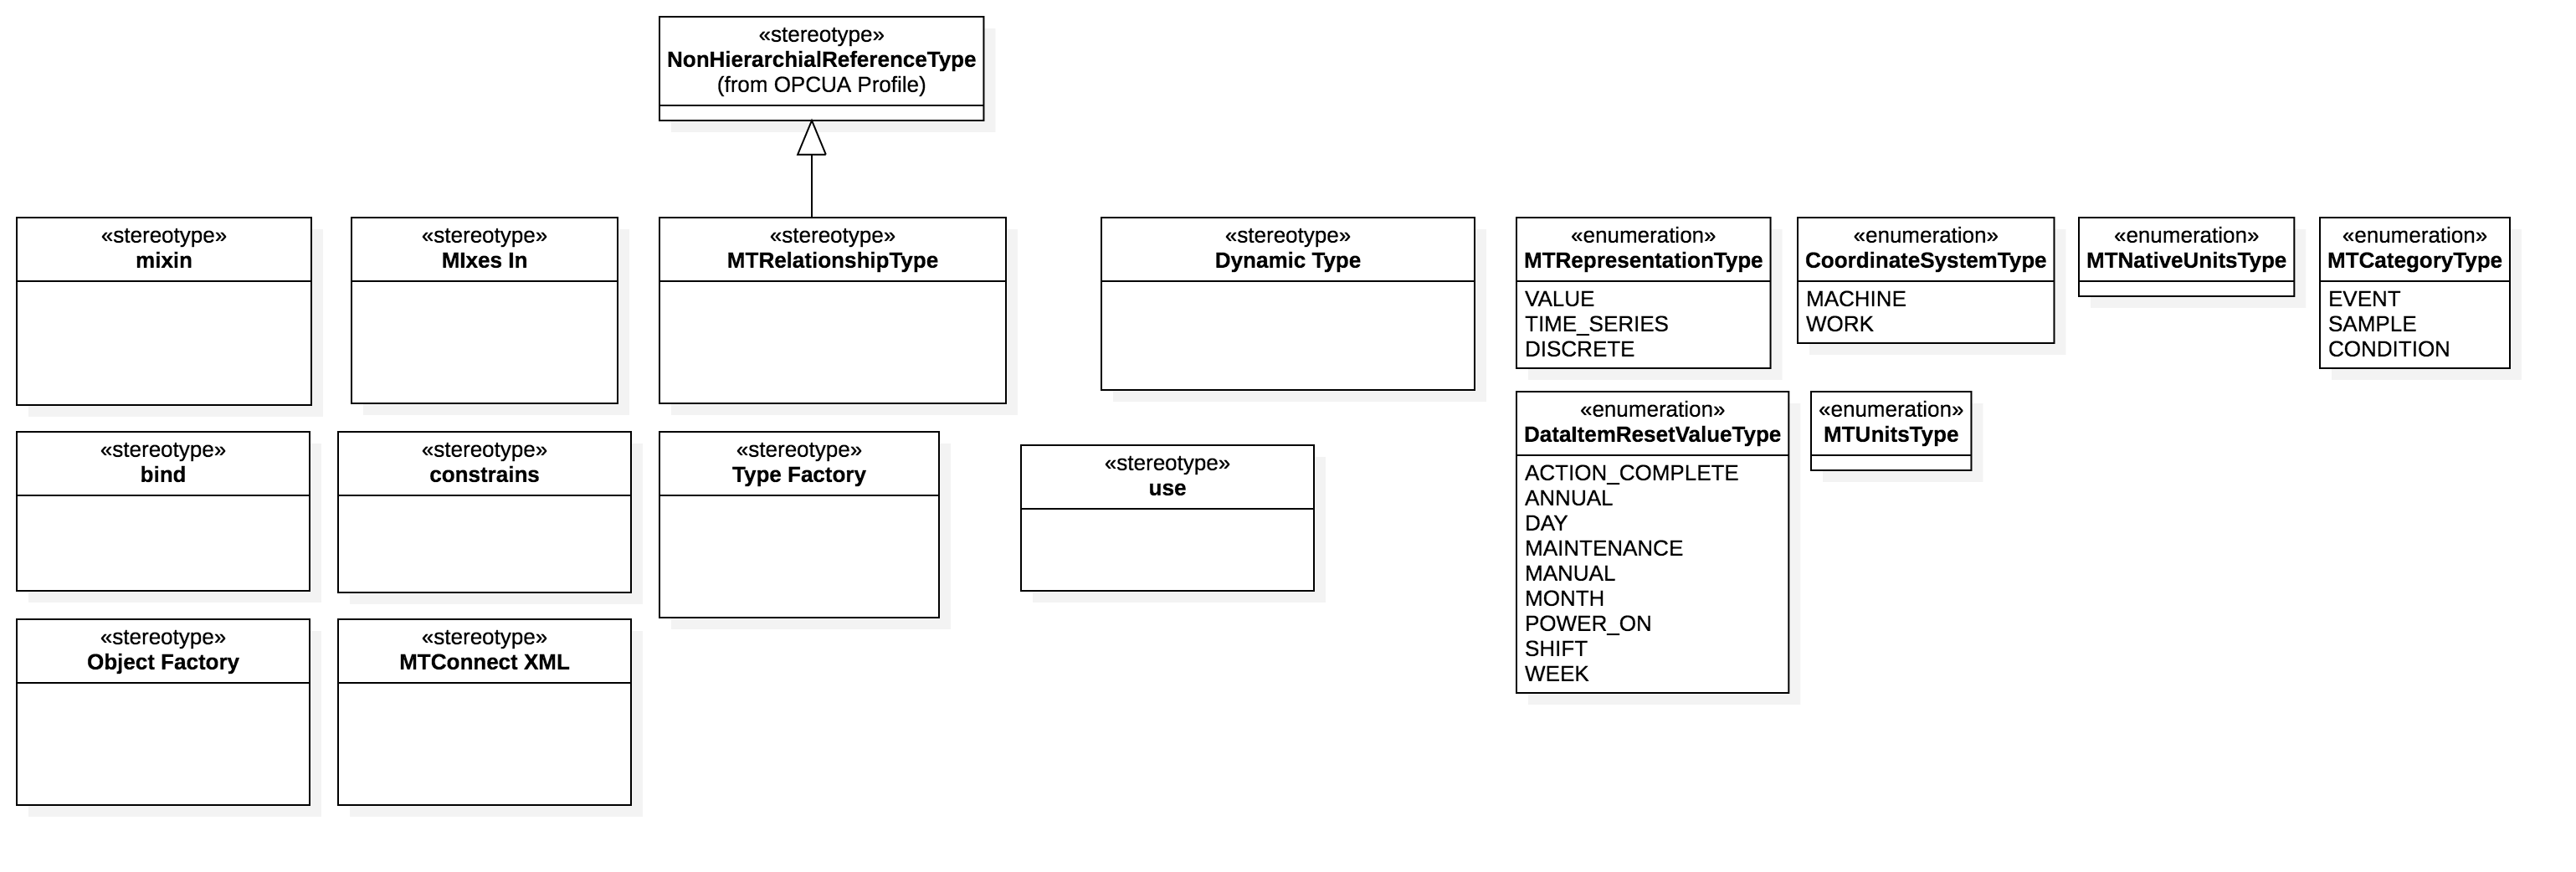
\includegraphics[width=1.0\textwidth]{./diagrams/types/MTConnectDeviceProfile.png}
  \caption{MTConnect Device Profile Diagram}
  \label{fig:MTConnectDeviceProfile}
\end{figure}

\FloatBarrier


The device profile documents the common data types and stereotypes that are 
used to construct the model. A stereotype is a design or modeling pattern that 
provides additional information about the type or the relationship between types. 

It can also identify the behavior of a property or the role the type or relation
will play in the model. 

Stereotypes are used throughout the model to provide additional information that 
will halp provide context and definition to aid in better understanding the
data model.

\subsubsection{Defintion of \texttt{ <<Deprecated>>}}
  \label{type:Deprecated}

\FloatBarrier

An MTConnect deprecated entity that is kept for backward compatibility.

\FloatBarrier
\subsubsection{Defintion of \texttt{ <<Dynamic Type>>}}
  \label{type:Dynamic Type}

\FloatBarrier

A dynamic type indicates that the class browse name and type will be 
determined at configuration time based on the MTConnect \gls{MTDevice}
elements.

\FloatBarrier
\subsubsection{Defintion of \texttt{ <<HasMTClassType>>}}
  \label{type:HasMTClassType}

\FloatBarrier

A \gls{MTDataItem} is representated in OPC UA as a sub-type of the most appropriate \uamodel{BaseDataVariableType}. 
The type is derived from the MTConnect \gls{type} attribute and references the corect \mtmodel{..ClassType}.

\begin{table}[ht]
\centering 
  \caption{\texttt{<<HasMTClassType>>} Definition}
  \label{table:HasMTClassType}
\fontsize{9pt}{11pt}\selectfont
\tabulinesep=3pt
\begin{tabu} to 6in {|X[-1.35]|X[-0.7]|X[-1.75]|X[-1.5]|X[-1]|X[-0.7]|} \everyrow{\hline}
\hline
\rowfont\bfseries {Attribute} & \multicolumn{5}{|l|}{Value} \\
\tabucline[1.5pt]{}
BrowseName & \multicolumn{5}{|l|}{HasMTClassType} \\
IsAbstract & \multicolumn{5}{|l|}{False} \\
Symmetric & \multicolumn{5}{|l|}{false} \\
\tabucline[1.5pt]{}
\rowfont \bfseries References & NodeClass & BrowseName & DataType & Type\-Definition & {Modeling\-Rule} \\
\multicolumn{6}{|l|}{Subtype of NonHierarchicalReferences (See \cite{UAPart5} Documentation)} \\
\end{tabu}
\end{table} 


\FloatBarrier
\subsubsection{Defintion of \texttt{ <<HasMTComposition>>}}
  \label{type:HasMTComposition}

\FloatBarrier

A reference from the MTConnect Data Item or condition to the Composition Object of the Component. 

\begin{table}[ht]
\centering 
  \caption{\texttt{<<HasMTComposition>>} Definition}
  \label{table:HasMTComposition}
\fontsize{9pt}{11pt}\selectfont
\tabulinesep=3pt
\begin{tabu} to 6in {|X[-1.35]|X[-0.7]|X[-1.75]|X[-1.5]|X[-1]|X[-0.7]|} \everyrow{\hline}
\hline
\rowfont\bfseries {Attribute} & \multicolumn{5}{|l|}{Value} \\
\tabucline[1.5pt]{}
BrowseName & \multicolumn{5}{|l|}{HasMTComposition} \\
IsAbstract & \multicolumn{5}{|l|}{False} \\
Symmetric & \multicolumn{5}{|l|}{true} \\
\tabucline[1.5pt]{}
\rowfont \bfseries References & NodeClass & BrowseName & DataType & Type\-Definition & {Modeling\-Rule} \\
\multicolumn{6}{|l|}{Subtype of NonHierarchicalReferences (See \cite{UAPart5} Documentation)} \\
\end{tabu}
\end{table} 


\FloatBarrier
\subsubsection{Defintion of \texttt{ <<HasMTReference>>}}
  \label{type:HasMTReference}

\FloatBarrier

A reference from one component to either a \gls{MTDataItem} or a \gls{MTComponent}.

\begin{table}[ht]
\centering 
  \caption{\texttt{<<HasMTReference>>} Definition}
  \label{table:HasMTReference}
\fontsize{9pt}{11pt}\selectfont
\tabulinesep=3pt
\begin{tabu} to 6in {|X[-1.35]|X[-0.7]|X[-1.75]|X[-1.5]|X[-1]|X[-0.7]|} \everyrow{\hline}
\hline
\rowfont\bfseries {Attribute} & \multicolumn{5}{|l|}{Value} \\
\tabucline[1.5pt]{}
BrowseName & \multicolumn{5}{|l|}{HasMTReference} \\
IsAbstract & \multicolumn{5}{|l|}{False} \\
Symmetric & \multicolumn{5}{|l|}{true} \\
\tabucline[1.5pt]{}
\rowfont \bfseries References & NodeClass & BrowseName & DataType & Type\-Definition & {Modeling\-Rule} \\
\multicolumn{6}{|l|}{Subtype of NonHierarchicalReferences (See \cite{UAPart5} Documentation)} \\
\end{tabu}
\end{table} 


\FloatBarrier
\subsubsection{Defintion of \texttt{ <<HasMTSource>>}}
  \label{type:HasMTSource}

\FloatBarrier

The \mtmodel{Source} relation to a \gls{MTComponent} or \gls{MTDataItem}.

\begin{table}[ht]
\centering 
  \caption{\texttt{<<HasMTSource>>} Definition}
  \label{table:HasMTSource}
\fontsize{9pt}{11pt}\selectfont
\tabulinesep=3pt
\begin{tabu} to 6in {|X[-1.35]|X[-0.7]|X[-1.75]|X[-1.5]|X[-1]|X[-0.7]|} \everyrow{\hline}
\hline
\rowfont\bfseries {Attribute} & \multicolumn{5}{|l|}{Value} \\
\tabucline[1.5pt]{}
BrowseName & \multicolumn{5}{|l|}{HasMTSource} \\
IsAbstract & \multicolumn{5}{|l|}{False} \\
Symmetric & \multicolumn{5}{|l|}{true} \\
\tabucline[1.5pt]{}
\rowfont \bfseries References & NodeClass & BrowseName & DataType & Type\-Definition & {Modeling\-Rule} \\
\multicolumn{6}{|l|}{Subtype of NonHierarchicalReferences (See \cite{UAPart5} Documentation)} \\
\end{tabu}
\end{table} 


\FloatBarrier
\subsubsection{Defintion of \texttt{ <<HasMTSubClassType>>}}
  \label{type:HasMTSubClassType}

\FloatBarrier

A \gls{MTDataItem} is representated in OPC UA as a sub-type of the most appropriate \uamodel{BaseDataVariableType}. 
The sub-type is derived from the MTConnect \gls{subType} attribute and references the corect \mtmodel{..ClassType}.

\begin{table}[ht]
\centering 
  \caption{\texttt{<<HasMTSubClassType>>} Definition}
  \label{table:HasMTSubClassType}
\fontsize{9pt}{11pt}\selectfont
\tabulinesep=3pt
\begin{tabu} to 6in {|X[-1.35]|X[-0.7]|X[-1.75]|X[-1.5]|X[-1]|X[-0.7]|} \everyrow{\hline}
\hline
\rowfont\bfseries {Attribute} & \multicolumn{5}{|l|}{Value} \\
\tabucline[1.5pt]{}
BrowseName & \multicolumn{5}{|l|}{HasMTSubClassType} \\
IsAbstract & \multicolumn{5}{|l|}{False} \\
Symmetric & \multicolumn{5}{|l|}{false} \\
\tabucline[1.5pt]{}
\rowfont \bfseries References & NodeClass & BrowseName & DataType & Type\-Definition & {Modeling\-Rule} \\
\multicolumn{6}{|l|}{Subtype of NonHierarchicalReferences (See \cite{UAPart5} Documentation)} \\
\end{tabu}
\end{table} 


\FloatBarrier
\subsubsection{Defintion of \texttt{ <<MTConnect XML>>}}
  \label{type:MTConnect XML}

\FloatBarrier

Tags an object as an MTConnect XML Element or Document that is used in a information flow
example.

\FloatBarrier
\subsubsection{Defintion of \texttt{ <<Mixes In>>}}
  \label{type:Mixes In}

\FloatBarrier

This stereotype is associated with the dependency between a type and a mixin. See Section \ref{type:mixin} for a complete 
description of the mixin.

\FloatBarrier
\subsubsection{Defintion of \texttt{ <<bind>>}}
  \label{type:bind}

\FloatBarrier

When a dynamic type (See Section \ref{type:Dynamic Type}) creates an instance where the super-type
can be associated based on the data item category and type, the \texttt{Type Factory} will 
specify which supertype is to be referenced.

The \texttt{bind} stereotype indicates the relationship between the dynamic sub-type and the 
parent type are resolved based on the MTConnect DataItem meta data.

\FloatBarrier
\subsubsection{Defintion of \texttt{ <<mixin>>}}
  \label{type:mixin}

\FloatBarrier

The mixin pattern injects the properties and operations into the types 
that are related to the using the \texttt{Mixes In} dependency. Mixins allow for
lightweight multiple inheritance. Since OPC/UA does not allow for multiple inheritance 
and the MTConnect  types require the same set of properties when they are sub-typed
from existing OPC/UA types, this mechanism allows for this relationship to be expressed.


\FloatBarrier
\subsubsection{Defintion of \texttt{ <<use>>}}
  \label{type:use}

\FloatBarrier

The use stereotype indicates that one class uses another as a helper to perform 
a specific operation or activity. This stereotype is mainly used to indicate
that a specific factory is being employed by another type to create dynamic
properties or relationships.

\FloatBarrier
\subsubsection{Defintion of \texttt{ <<values>>}}
  \label{type:values}

\FloatBarrier

For controlled vocabularies of enumerated types, specifies the relationship to the allowable 
values for the type.

\FloatBarrier
